\documentclass[aspectratio=169,professionalfont,xcolor={dvipsnames},hyperref={colorlinks=true,urlcolor=MidnightBlue}]{beamer}

\usepackage{bm}
\usepackage{tikz}
\usepackage{mathtools}
\usetikzlibrary{%
  arrows,%
  backgrounds,
  intersections,
  shapes,
  shapes.misc,% wg. rounded rectangle
  shapes.arrows,%
  chains,%
  matrix,%
  positioning,% wg. " of "
  scopes,%
  decorations.pathmorphing,% /pgf/decoration/random steps | erste Graphik
  shadows,%
  patterns% for hatched rect
}
\usepackage{pgfplots}
\usepackage[bitstream-charter]{mathdesign}
\usetheme{simple}

\newcommand{\abs}{\,\mathrm{abs}}
\newcommand{\add}{\,\mathrm{add}}
\newcommand{\bin}{\,\mathrm{bin}}
\newcommand{\sign}{\,\mathrm{sign}}
\newcommand{\mult}{\,\mathrm{mult}}
\newcommand{\gate}{\,\mathrm{gate}}
\newcommand{\tanhs}{\,\mathrm{tanh}\sigma}
\newcommand{\Wre}{\bm W_r}
\newcommand{\Wim}{\bm W_i}
\newcommand{\real}{\mathrm{real}}
\newcommand{\logc}{\mathrm{log}_{\mathbb{C}}}

\begin{document}
{
  \setbeamertemplate{background}
  {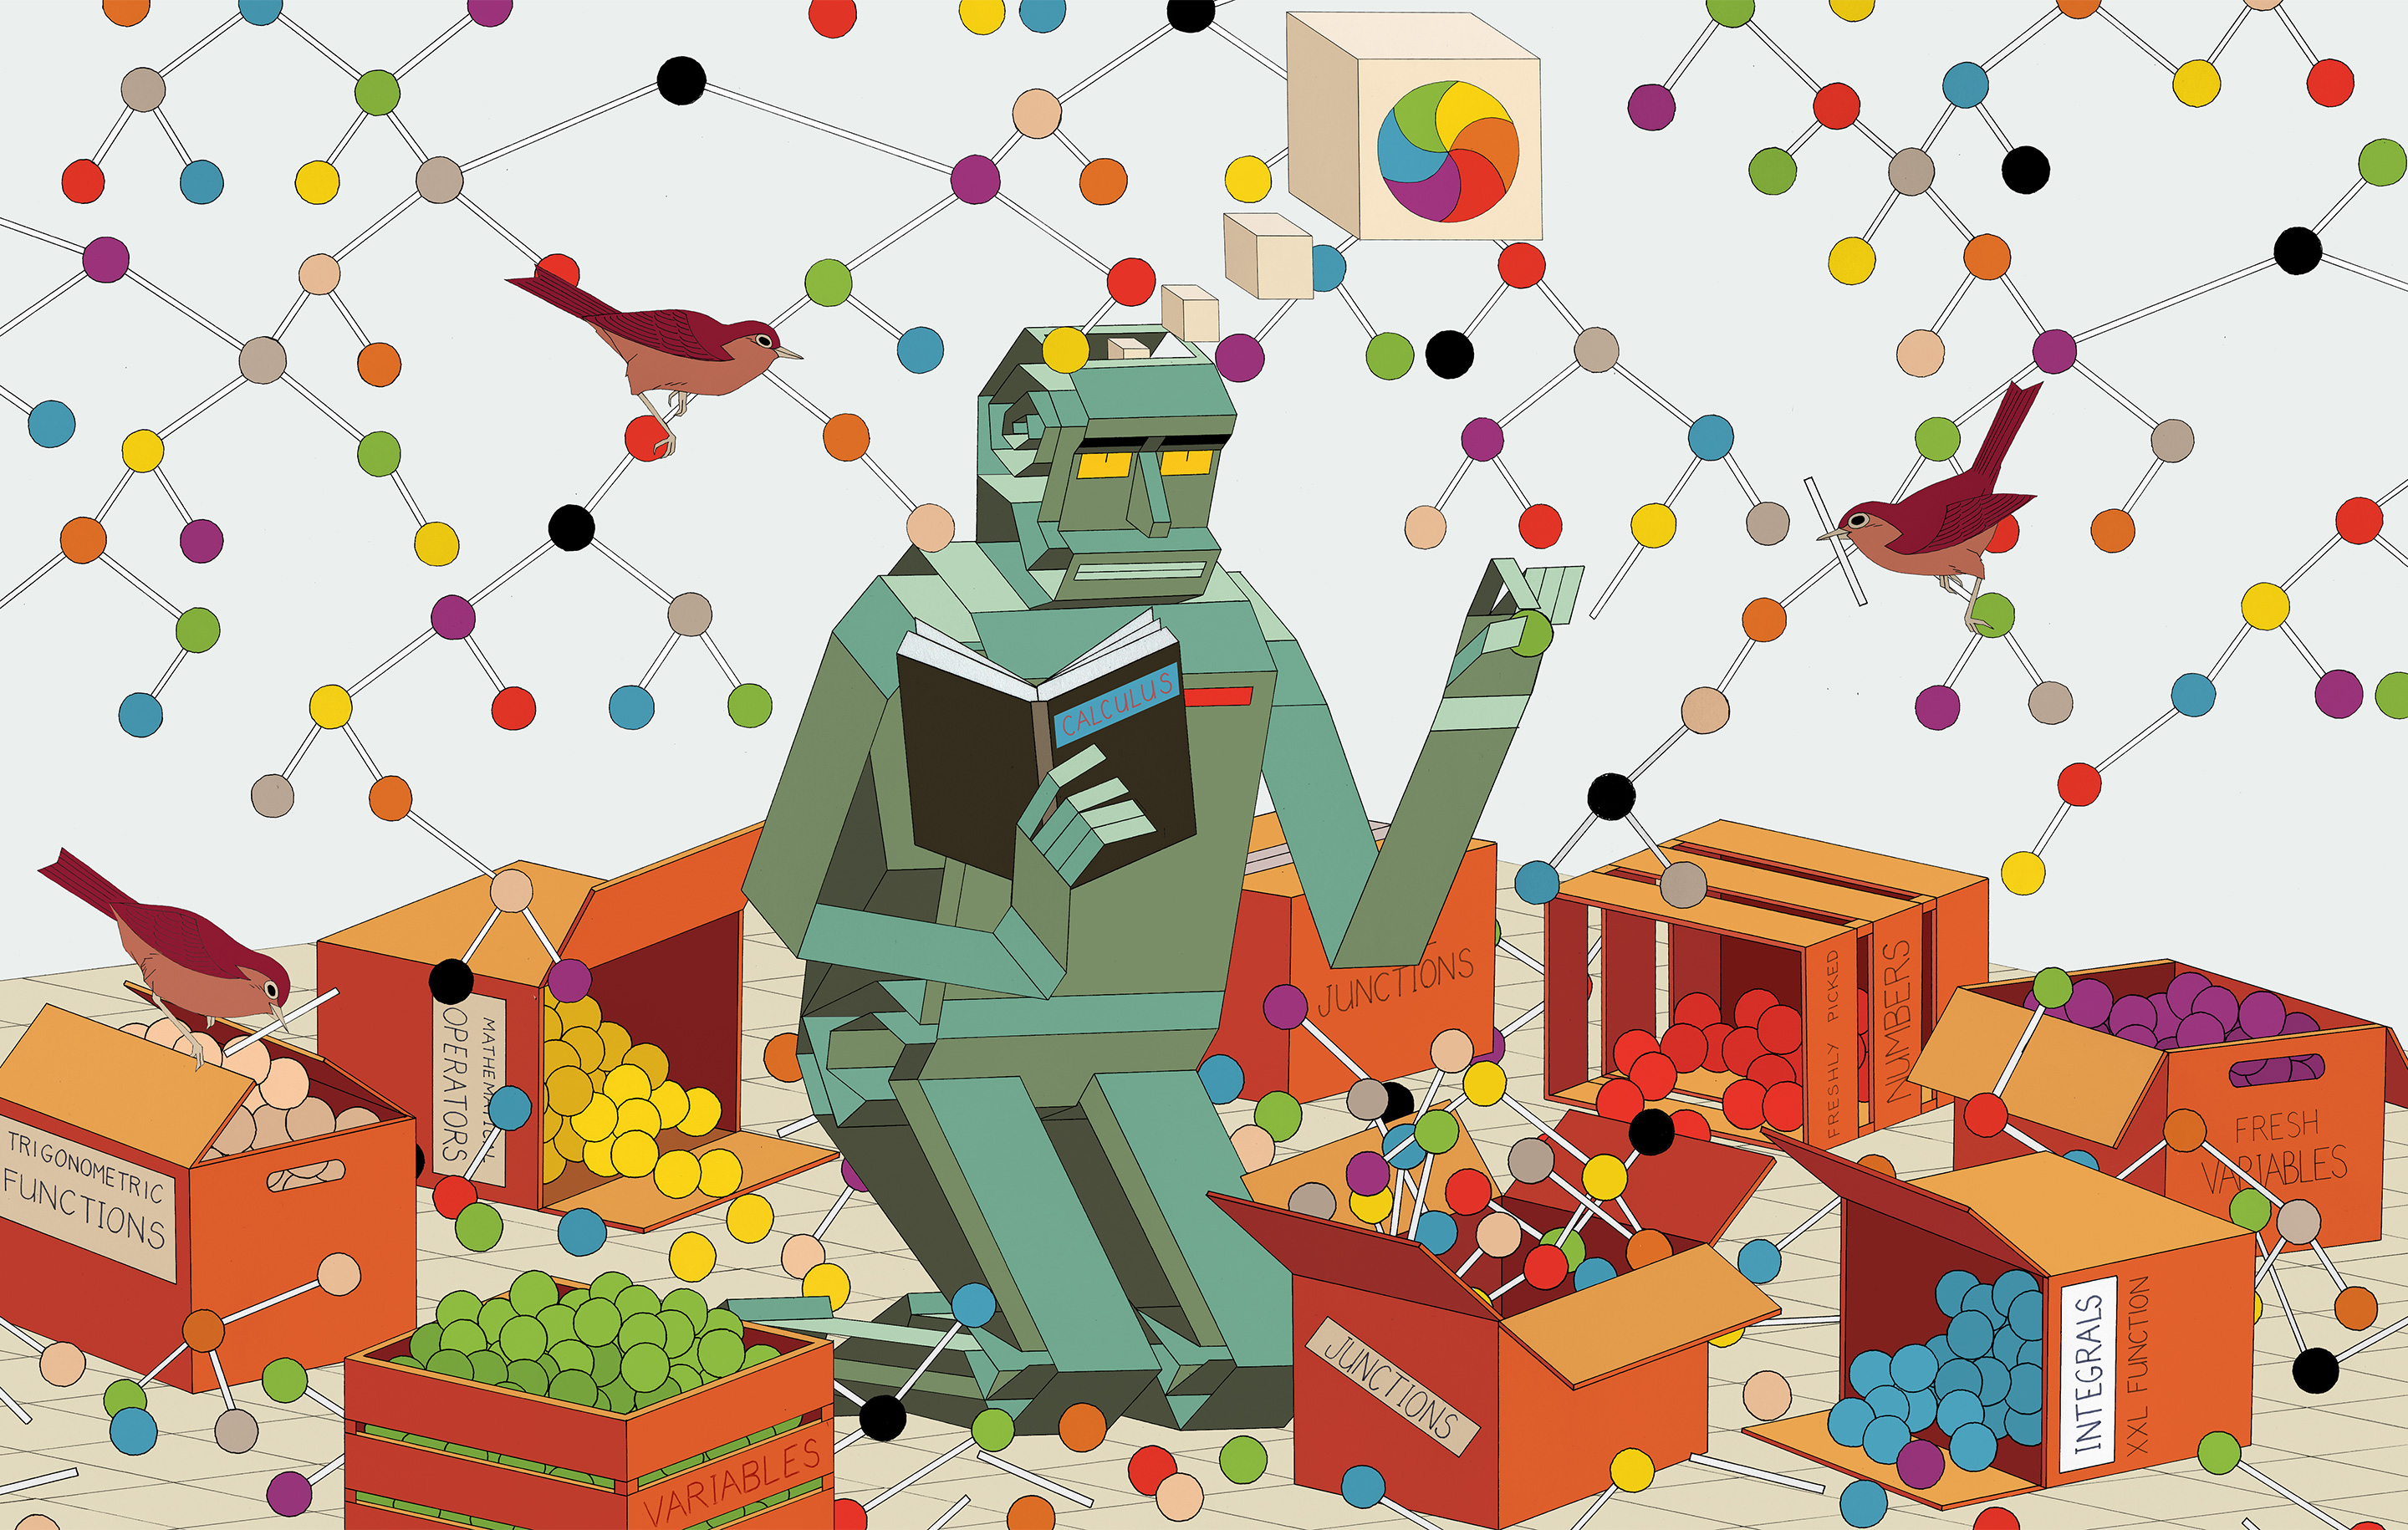
\includegraphics[width = \the\paperwidth, height = \the\paperheight]{robot-math.jpg}}
  \begin{frame}
    \vspace{-0.1cm}
    \begin{center}
      
\begin{tikzpicture}[
          box/.style={fill=white,fill opacity=0.5,text opacity=1,minimum width=\paperwidth, overlay}]
        \node[box] (title) at (0,0) {\Huge\bf Neural Arithmetic};
        \node[box] (subtitle) at (0,-0.836) {\large\bf Teaching Math To Neural Networks?};
      \end{tikzpicture}
    \end{center}
    \vspace{7.5cm}\hspace{-1cm}
    {\tiny Source: \href{
      https://www.quantamagazine.org/symbolic-mathematics-finally-yields-to-neural-networks-20200520/}{\underline{Quanta Magazine}}}
  \end{frame}
}

\begin{frame}
  \centering
  {\huge\bf Neural Arithmetic} \\
  \vspace{.5cm}
  \textbf{Extrapolating} Beyond The Training Range \\
  \& Building \textbf{Transparent} Models
\end{frame}

\begin{frame}{Neural Networks}
  \begin{columns}
    \column{.5\textwidth}\centering
    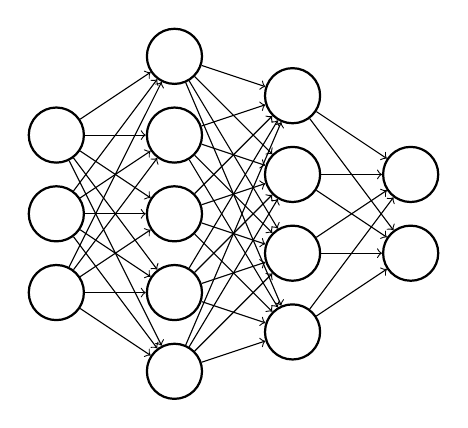
\begin{tikzpicture}[
    neuron/.style={circle, minimum size=.7cm, thick},
    tip/.style={->}
  ]
  % draw neurons
  \node[neuron, draw] at (-1.5,1) (11) {};
  \node[neuron, draw] at (-1.5,0) (12) {};
  \node[neuron, draw] at (-1.5,-1) (13) {};
  \foreach \n in {21,...,25}{
    \node[neuron, draw] at (0, \n - 23) (\n) {};}
  \foreach \n in {31,...,34}{
    \node[neuron, draw] at (1.5,\n-32.5) (\n) {};}
  \foreach \n in {41,...,42}{
    \node[neuron, draw] at (3.0,\n-41.5) (\n) {};}

  % draw connections
  \foreach \idx in {11,...,13}{
    \foreach \jdx in {21,...,25}{
      \path[draw,tip] (\idx) edge (\jdx) node {};}}
  \foreach \idx in {21,...,25}{
    \foreach \jdx in {31,...,34}{
      \path[draw,tip] (\idx) edge (\jdx) node {};}}
  \foreach \idx in {31,...,34}{
    \foreach \jdx in {41,...,42}{
      \path[draw,tip] (\idx) edge (\jdx) node {};}}
\end{tikzpicture}


    \column{.5\textwidth}\centering
    Composed of \textbf{Dense} layers:
    \begin{equation*}
      \bm y = \sigma(\bm W\bm x + \bm b)
    \end{equation*}
    {\tiny (No convolutions in this talk.)}
  \end{columns}
\end{frame}

\begin{frame}{Neural Networks}
  \begin{columns}
    \column{.33\textwidth}\centering
    \resizebox{!}{\textwidth}{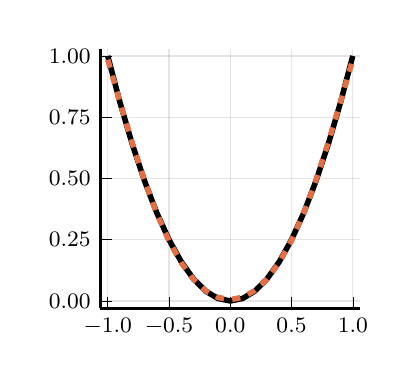
\begin{tikzpicture}[/tikz/background rectangle/.style={fill={rgb,1:red,1.0;green,1.0;blue,1.0}, draw opacity={1.0}}, show background rectangle]
\begin{axis}[point meta max={nan}, point meta min={nan}, legend cell align={left}, title={}, title style={at={{(0.5,1)}}, anchor={south}, font={{\fontsize{14 pt}{18.2 pt}\selectfont}}, color={rgb,1:red,0.0;green,0.0;blue,0.0}, draw opacity={1.0}, rotate={0.0}}, legend style={color={rgb,1:red,0.0;green,0.0;blue,0.0}, draw opacity={1.0}, line width={1}, solid, fill={rgb,1:red,1.0;green,1.0;blue,1.0}, fill opacity={1.0}, text opacity={1.0}, font={{\fontsize{8 pt}{10.4 pt}\selectfont}}, at={(1.02, 1)}, anchor={north west}}, axis background/.style={fill={rgb,1:red,1.0;green,1.0;blue,1.0}, opacity={1.0}}, anchor={north west}, xshift={1.0mm}, yshift={-1.0mm}, width={48.8mm}, height={48.8mm}, scaled x ticks={false}, xlabel={}, x tick style={color={rgb,1:red,0.0;green,0.0;blue,0.0}, opacity={1.0}}, x tick label style={color={rgb,1:red,0.0;green,0.0;blue,0.0}, opacity={1.0}, rotate={0}}, xlabel style={at={(ticklabel cs:0.5)}, anchor=near ticklabel, font={{\fontsize{11 pt}{14.3 pt}\selectfont}}, color={rgb,1:red,0.0;green,0.0;blue,0.0}, draw opacity={1.0}, rotate={0.0}}, xmajorgrids={true}, xmin={-1.06}, xmax={1.06}, xtick={{-1.0,-0.5,0.0,0.5,1.0}}, xticklabels={{$-1.0$,$-0.5$,$0.0$,$0.5$,$1.0$}}, xtick align={inside}, xticklabel style={font={{\fontsize{8 pt}{10.4 pt}\selectfont}}, color={rgb,1:red,0.0;green,0.0;blue,0.0}, draw opacity={1.0}, rotate={0.0}}, x grid style={color={rgb,1:red,0.0;green,0.0;blue,0.0}, draw opacity={0.1}, line width={0.5}, solid}, axis x line*={left}, x axis line style={color={rgb,1:red,0.0;green,0.0;blue,0.0}, draw opacity={1.0}, line width={1}, solid}, scaled y ticks={false}, ylabel={}, y tick style={color={rgb,1:red,0.0;green,0.0;blue,0.0}, opacity={1.0}}, y tick label style={color={rgb,1:red,0.0;green,0.0;blue,0.0}, opacity={1.0}, rotate={0}}, ylabel style={at={(ticklabel cs:0.5)}, anchor=near ticklabel, font={{\fontsize{11 pt}{14.3 pt}\selectfont}}, color={rgb,1:red,0.0;green,0.0;blue,0.0}, draw opacity={1.0}, rotate={0.0}}, ymajorgrids={true}, ymin={-0.03}, ymax={1.03}, ytick={{0.0,0.25,0.5,0.75,1.0}}, yticklabels={{$0.00$,$0.25$,$0.50$,$0.75$,$1.00$}}, ytick align={inside}, yticklabel style={font={{\fontsize{8 pt}{10.4 pt}\selectfont}}, color={rgb,1:red,0.0;green,0.0;blue,0.0}, draw opacity={1.0}, rotate={0.0}}, y grid style={color={rgb,1:red,0.0;green,0.0;blue,0.0}, draw opacity={0.1}, line width={0.5}, solid}, axis y line*={left}, y axis line style={color={rgb,1:red,0.0;green,0.0;blue,0.0}, draw opacity={1.0}, line width={1}, solid}]
    \addplot[color={rgb,1:red,0.0;green,0.0;blue,0.0}, name path={d1cbcbfa-7c7d-4d45-af38-95e66fc16208}, draw opacity={1.0}, line width={2}, solid]
        table[row sep={\\}]
        {
            \\
            -1.0  1.0  \\
            -0.9  0.81  \\
            -0.8  0.6400000000000001  \\
            -0.7  0.48999999999999994  \\
            -0.6  0.36  \\
            -0.5  0.25  \\
            -0.4  0.16000000000000003  \\
            -0.3  0.09  \\
            -0.2  0.04000000000000001  \\
            -0.1  0.010000000000000002  \\
            0.0  0.0  \\
            0.1  0.010000000000000002  \\
            0.2  0.04000000000000001  \\
            0.3  0.09  \\
            0.4  0.16000000000000003  \\
            0.5  0.25  \\
            0.6  0.36  \\
            0.7  0.48999999999999994  \\
            0.8  0.6400000000000001  \\
            0.9  0.81  \\
            1.0  1.0  \\
        }
        ;
    \addplot[color={rgb,1:red,0.8889;green,0.4356;blue,0.2781}, name path={ed266a9f-d390-4427-baf0-d5db462149f8}, draw opacity={1.0}, line width={2}, dashed]
        table[row sep={\\}]
        {
            \\
            -1.0  0.9845725893974304  \\
            -0.9  0.8106645941734314  \\
            -0.8  0.6438924670219421  \\
            -0.7  0.49109119176864624  \\
            -0.6  0.35722726583480835  \\
            -0.5  0.24509257078170776  \\
            -0.4  0.15554028749465942  \\
            -0.3  0.08804923295974731  \\
            -0.2  0.04138833284378052  \\
            -0.1  0.01420825719833374  \\
            0.0  0.005487382411956787  \\
            0.1  0.01480323076248169  \\
            0.2  0.042453229427337646  \\
            0.3  0.08940249681472778  \\
            0.4  0.15705054998397827  \\
            0.5  0.24677687883377075  \\
            0.6  0.3592577576637268  \\
            0.7  0.49364858865737915  \\
            0.8  0.6468579173088074  \\
            0.9  0.8132650256156921  \\
            1.0  0.9851908683776855  \\
        }
        ;
\end{axis}
\end{tikzpicture}
}
    Universal \textbf{Approximators} 

    \pause
    \column{.33\textwidth}\centering
    \resizebox{!}{\textwidth}{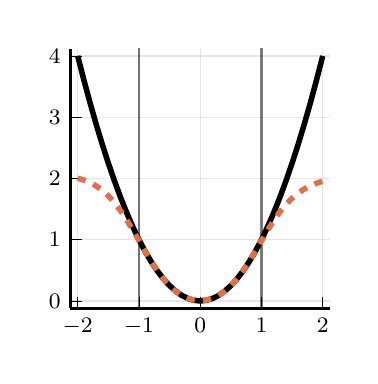
\begin{tikzpicture}[/tikz/background rectangle/.style={fill={rgb,1:red,1.0;green,1.0;blue,1.0}, draw opacity={1.0}}, show background rectangle]
\begin{axis}[point meta max={nan}, point meta min={nan}, legend cell align={left}, title={}, title style={at={{(0.5,1)}}, anchor={south}, font={{\fontsize{14 pt}{18.2 pt}\selectfont}}, color={rgb,1:red,0.0;green,0.0;blue,0.0}, draw opacity={1.0}, rotate={0.0}}, legend style={color={rgb,1:red,0.0;green,0.0;blue,0.0}, draw opacity={1.0}, line width={1}, solid, fill={rgb,1:red,1.0;green,1.0;blue,1.0}, fill opacity={1.0}, text opacity={1.0}, font={{\fontsize{8 pt}{10.4 pt}\selectfont}}, at={(1.02, 1)}, anchor={north west}}, axis background/.style={fill={rgb,1:red,1.0;green,1.0;blue,1.0}, opacity={1.0}}, anchor={north west}, xshift={1.0mm}, yshift={-1.0mm}, width={48.8mm}, height={48.8mm}, scaled x ticks={false}, xlabel={}, x tick style={color={rgb,1:red,0.0;green,0.0;blue,0.0}, opacity={1.0}}, x tick label style={color={rgb,1:red,0.0;green,0.0;blue,0.0}, opacity={1.0}, rotate={0}}, xlabel style={at={(ticklabel cs:0.5)}, anchor=near ticklabel, font={{\fontsize{11 pt}{14.3 pt}\selectfont}}, color={rgb,1:red,0.0;green,0.0;blue,0.0}, draw opacity={1.0}, rotate={0.0}}, xmajorgrids={true}, xmin={-2.12}, xmax={2.12}, xtick={{-2.0,-1.0,0.0,1.0,2.0}}, xticklabels={{$-2$,$-1$,$0$,$1$,$2$}}, xtick align={inside}, xticklabel style={font={{\fontsize{8 pt}{10.4 pt}\selectfont}}, color={rgb,1:red,0.0;green,0.0;blue,0.0}, draw opacity={1.0}, rotate={0.0}}, x grid style={color={rgb,1:red,0.0;green,0.0;blue,0.0}, draw opacity={0.1}, line width={0.5}, solid}, axis x line*={left}, x axis line style={color={rgb,1:red,0.0;green,0.0;blue,0.0}, draw opacity={1.0}, line width={1}, solid}, scaled y ticks={false}, ylabel={}, y tick style={color={rgb,1:red,0.0;green,0.0;blue,0.0}, opacity={1.0}}, y tick label style={color={rgb,1:red,0.0;green,0.0;blue,0.0}, opacity={1.0}, rotate={0}}, ylabel style={at={(ticklabel cs:0.5)}, anchor=near ticklabel, font={{\fontsize{11 pt}{14.3 pt}\selectfont}}, color={rgb,1:red,0.0;green,0.0;blue,0.0}, draw opacity={1.0}, rotate={0.0}}, ymajorgrids={true}, ymin={-0.12}, ymax={4.12}, ytick={{0.0,1.0,2.0,3.0,4.0}}, yticklabels={{$0$,$1$,$2$,$3$,$4$}}, ytick align={inside}, yticklabel style={font={{\fontsize{8 pt}{10.4 pt}\selectfont}}, color={rgb,1:red,0.0;green,0.0;blue,0.0}, draw opacity={1.0}, rotate={0.0}}, y grid style={color={rgb,1:red,0.0;green,0.0;blue,0.0}, draw opacity={0.1}, line width={0.5}, solid}, axis y line*={left}, y axis line style={color={rgb,1:red,0.0;green,0.0;blue,0.0}, draw opacity={1.0}, line width={1}, solid}]
    \addplot[color={rgb,1:red,0.0;green,0.0;blue,0.0}, name path={7b52b317-e8cc-495b-91cf-5057389872ce}, draw opacity={1.0}, line width={2}, solid]
        table[row sep={\\}]
        {
            \\
            -2.0  4.0  \\
            -1.9  3.61  \\
            -1.8  3.24  \\
            -1.7  2.8899999999999997  \\
            -1.6  2.5600000000000005  \\
            -1.5  2.25  \\
            -1.4  1.9599999999999997  \\
            -1.3  1.6900000000000002  \\
            -1.2  1.44  \\
            -1.1  1.2100000000000002  \\
            -1.0  1.0  \\
            -0.9  0.81  \\
            -0.8  0.6400000000000001  \\
            -0.7  0.48999999999999994  \\
            -0.6  0.36  \\
            -0.5  0.25  \\
            -0.4  0.16000000000000003  \\
            -0.3  0.09  \\
            -0.2  0.04000000000000001  \\
            -0.1  0.010000000000000002  \\
            0.0  0.0  \\
            0.1  0.010000000000000002  \\
            0.2  0.04000000000000001  \\
            0.3  0.09  \\
            0.4  0.16000000000000003  \\
            0.5  0.25  \\
            0.6  0.36  \\
            0.7  0.48999999999999994  \\
            0.8  0.6400000000000001  \\
            0.9  0.81  \\
            1.0  1.0  \\
            1.1  1.2100000000000002  \\
            1.2  1.44  \\
            1.3  1.6900000000000002  \\
            1.4  1.9599999999999997  \\
            1.5  2.25  \\
            1.6  2.5600000000000005  \\
            1.7  2.8899999999999997  \\
            1.8  3.24  \\
            1.9  3.61  \\
            2.0  4.0  \\
        }
        ;
    \addplot[color={rgb,1:red,0.0;green,0.0;blue,0.0}, name path={6b43bb21-6878-4d76-abeb-37fcce96b338}, draw opacity={0.5}, line width={1}, solid]
        table[row sep={\\}]
        {
            \\
            -1.0  -4.36  \\
            -1.0  8.36  \\
        }
        ;
    \addplot[color={rgb,1:red,0.0;green,0.0;blue,0.0}, name path={6b43bb21-6878-4d76-abeb-37fcce96b338}, draw opacity={0.5}, line width={1}, solid]
        table[row sep={\\}]
        {
            \\
            1.0  -4.36  \\
            1.0  8.36  \\
        }
        ;
    \addplot[color={rgb,1:red,0.8889;green,0.4356;blue,0.2781}, name path={3fbd8df0-cce3-4d0f-be53-09e781260df2}, draw opacity={1.0}, line width={2}, dashed]
        table[row sep={\\}]
        {
            \\
            -2.0  2.0036094188690186  \\
            -1.9  1.974085807800293  \\
            -1.8  1.9330570697784424  \\
            -1.7  1.8779866695404053  \\
            -1.6  1.8062870502471924  \\
            -1.5  1.715660572052002  \\
            -1.4  1.6045968532562256  \\
            -1.3  1.472982406616211  \\
            -1.2  1.3226659297943115  \\
            -1.1  1.1577801704406738  \\
            -1.0  0.9845725893974304  \\
            -0.9  0.8106645941734314  \\
            -0.8  0.6438924670219421  \\
            -0.7  0.49109119176864624  \\
            -0.6  0.35722726583480835  \\
            -0.5  0.24509257078170776  \\
            -0.4  0.15554028749465942  \\
            -0.3  0.08804923295974731  \\
            -0.2  0.04138833284378052  \\
            -0.1  0.01420825719833374  \\
            0.0  0.005487382411956787  \\
            0.1  0.01480323076248169  \\
            0.2  0.042453229427337646  \\
            0.3  0.08940249681472778  \\
            0.4  0.15705054998397827  \\
            0.5  0.24677687883377075  \\
            0.6  0.3592577576637268  \\
            0.7  0.49364858865737915  \\
            0.8  0.6468579173088074  \\
            0.9  0.8132650256156921  \\
            1.0  0.9851908683776855  \\
            1.1  1.1541205644607544  \\
            1.2  1.312281847000122  \\
            1.3  1.4539601802825928  \\
            1.4  1.5761010646820068  \\
            1.5  1.678144931793213  \\
            1.6  1.761376142501831  \\
            1.7  1.8281397819519043  \\
            1.8  1.8811771869659424  \\
            1.9  1.9231770038604736  \\
            2.0  1.9565298557281494  \\
        }
        ;
\end{axis}
\end{tikzpicture}
}
    Poor \textbf{Extrapolators} 

    \pause
    \column{.33\textwidth}\centering
    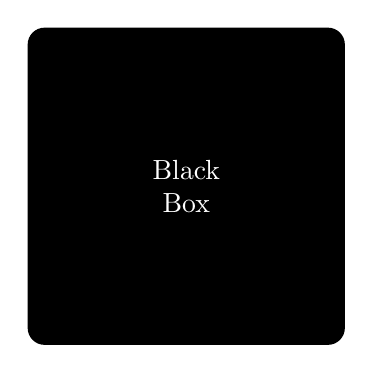
\begin{tikzpicture}[box/.style={
        draw,thick,
        minimum height=4cm,
        minimum width=4cm,
        rounded corners=0.2cm,
        align=center,fill=black,
        text=white
    }]
      \node[box] (b) {Black\\Box};
    \end{tikzpicture}\\
    \vspace{.6cm}
    \textbf{Intransparent}
    
  \end{columns}
\end{frame}

\begin{frame}{Problems With Extrapolation}
  \resizebox{\textwidth}{!}{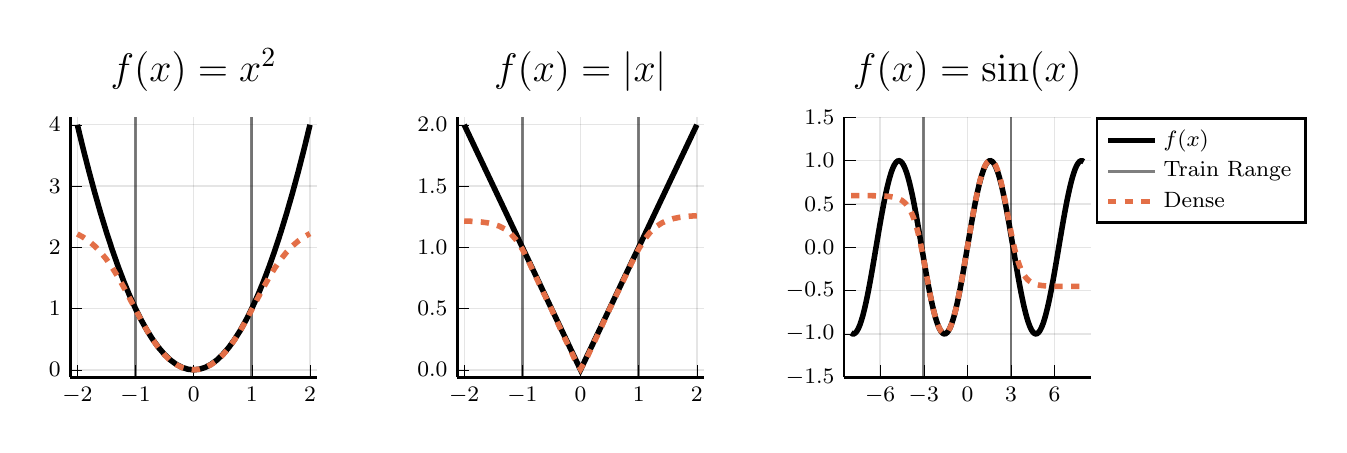
\begin{tikzpicture}[/tikz/background rectangle/.style={fill={rgb,1:red,1.0;green,1.0;blue,1.0}, draw opacity={1.0}}, show background rectangle]
\begin{axis}[point meta max={nan}, point meta min={nan}, legend cell align={left}, title={$f(x) = x^2$}, title style={at={{(0.5,1)}}, anchor={south}, font={{\fontsize{14 pt}{18.2 pt}\selectfont}}, color={rgb,1:red,0.0;green,0.0;blue,0.0}, draw opacity={1.0}, rotate={0.0}}, legend style={color={rgb,1:red,0.0;green,0.0;blue,0.0}, draw opacity={1.0}, line width={1}, solid, fill={rgb,1:red,1.0;green,1.0;blue,1.0}, fill opacity={1.0}, text opacity={1.0}, font={{\fontsize{8 pt}{10.4 pt}\selectfont}}, at={(1.02, 1)}, anchor={north west}}, axis background/.style={fill={rgb,1:red,1.0;green,1.0;blue,1.0}, opacity={1.0}}, anchor={north west}, xshift={1.0mm}, yshift={-1.0mm}, width={47.13333333333333mm}, height={48.8mm}, scaled x ticks={false}, xlabel={}, x tick style={color={rgb,1:red,0.0;green,0.0;blue,0.0}, opacity={1.0}}, x tick label style={color={rgb,1:red,0.0;green,0.0;blue,0.0}, opacity={1.0}, rotate={0}}, xlabel style={at={(ticklabel cs:0.5)}, anchor=near ticklabel, font={{\fontsize{11 pt}{14.3 pt}\selectfont}}, color={rgb,1:red,0.0;green,0.0;blue,0.0}, draw opacity={1.0}, rotate={0.0}}, xmajorgrids={true}, xmin={-2.12}, xmax={2.12}, xtick={{-2.0,-1.0,0.0,1.0,2.0}}, xticklabels={{$-2$,$-1$,$0$,$1$,$2$}}, xtick align={inside}, xticklabel style={font={{\fontsize{8 pt}{10.4 pt}\selectfont}}, color={rgb,1:red,0.0;green,0.0;blue,0.0}, draw opacity={1.0}, rotate={0.0}}, x grid style={color={rgb,1:red,0.0;green,0.0;blue,0.0}, draw opacity={0.1}, line width={0.5}, solid}, axis x line*={left}, x axis line style={color={rgb,1:red,0.0;green,0.0;blue,0.0}, draw opacity={1.0}, line width={1}, solid}, scaled y ticks={false}, ylabel={}, y tick style={color={rgb,1:red,0.0;green,0.0;blue,0.0}, opacity={1.0}}, y tick label style={color={rgb,1:red,0.0;green,0.0;blue,0.0}, opacity={1.0}, rotate={0}}, ylabel style={at={(ticklabel cs:0.5)}, anchor=near ticklabel, font={{\fontsize{11 pt}{14.3 pt}\selectfont}}, color={rgb,1:red,0.0;green,0.0;blue,0.0}, draw opacity={1.0}, rotate={0.0}}, ymajorgrids={true}, ymin={-0.12}, ymax={4.12}, ytick={{0.0,1.0,2.0,3.0,4.0}}, yticklabels={{$0$,$1$,$2$,$3$,$4$}}, ytick align={inside}, yticklabel style={font={{\fontsize{8 pt}{10.4 pt}\selectfont}}, color={rgb,1:red,0.0;green,0.0;blue,0.0}, draw opacity={1.0}, rotate={0.0}}, y grid style={color={rgb,1:red,0.0;green,0.0;blue,0.0}, draw opacity={0.1}, line width={0.5}, solid}, axis y line*={left}, y axis line style={color={rgb,1:red,0.0;green,0.0;blue,0.0}, draw opacity={1.0}, line width={1}, solid}]
    \addplot[color={rgb,1:red,0.0;green,0.0;blue,0.0}, name path={40310bec-3aa3-4e7e-9624-8a98ce448685}, draw opacity={1.0}, line width={2}, solid]
        table[row sep={\\}]
        {
            \\
            -2.0  4.0  \\
            -1.9  3.61  \\
            -1.8  3.2399998  \\
            -1.7  2.89  \\
            -1.6  2.5600002  \\
            -1.5  2.25  \\
            -1.4  1.9599999  \\
            -1.3  1.6899998  \\
            -1.2  1.44  \\
            -1.1  1.21  \\
            -1.0  1.0  \\
            -0.9  0.80999994  \\
            -0.8  0.64000005  \\
            -0.7  0.48999998  \\
            -0.6  0.36  \\
            -0.5  0.25  \\
            -0.4  0.16000001  \\
            -0.3  0.09  \\
            -0.2  0.040000003  \\
            -0.1  0.010000001  \\
            0.0  0.0  \\
            0.1  0.010000001  \\
            0.2  0.040000003  \\
            0.3  0.09  \\
            0.4  0.16000001  \\
            0.5  0.25  \\
            0.6  0.36  \\
            0.7  0.48999998  \\
            0.8  0.64000005  \\
            0.9  0.80999994  \\
            1.0  1.0  \\
            1.1  1.21  \\
            1.2  1.44  \\
            1.3  1.6899998  \\
            1.4  1.9599999  \\
            1.5  2.25  \\
            1.6  2.5600002  \\
            1.7  2.89  \\
            1.8  3.2399998  \\
            1.9  3.61  \\
            2.0  4.0  \\
        }
        ;
    \addplot[color={rgb,1:red,0.0;green,0.0;blue,0.0}, name path={7c0581ae-dc7e-413f-9b93-3ecf2569d53d}, draw opacity={0.5}, line width={1}, solid]
        table[row sep={\\}]
        {
            \\
            -1.0  -4.36  \\
            -1.0  8.36  \\
        }
        ;
    \addplot[color={rgb,1:red,0.0;green,0.0;blue,0.0}, name path={7c0581ae-dc7e-413f-9b93-3ecf2569d53d}, draw opacity={0.5}, line width={1}, solid]
        table[row sep={\\}]
        {
            \\
            1.0  -4.36  \\
            1.0  8.36  \\
        }
        ;
    \addplot[color={rgb,1:red,0.8889;green,0.4356;blue,0.2781}, name path={7f6b1272-9520-43ea-a88d-901d48bbec28}, draw opacity={1.0}, line width={2}, dashed]
        table[row sep={\\}]
        {
            \\
            -2.0  2.2175353  \\
            -1.9  2.1652787  \\
            -1.8  2.0999224  \\
            -1.7  2.0192063  \\
            -1.6  1.9211061  \\
            -1.5  1.8042185  \\
            -1.4  1.6682322  \\
            -1.3  1.5143886  \\
            -1.2  1.3457947  \\
            -1.1  1.1674106  \\
            -1.0  0.9856209  \\
            -0.9  0.8074259  \\
            -0.8  0.6394708  \\
            -0.7  0.4871961  \\
            -0.6  0.35434574  \\
            -0.5  0.24290484  \\
            -0.4  0.1533894  \\
            -0.3  0.08532515  \\
            -0.2  0.037757277  \\
            -0.1  0.0096870065  \\
            0.0  0.00038653612  \\
            0.1  0.009584248  \\
            0.2  0.037525535  \\
            0.3  0.08491385  \\
            0.4  0.1527282  \\
            0.5  0.24191368  \\
            0.6  0.3529526  \\
            0.7  0.4853617  \\
            0.8  0.63721913  \\
            0.9  0.8048696  \\
            1.0  0.9829703  \\
            1.1  1.1649592  \\
            1.2  1.3438771  \\
            1.3  1.5133243  \\
            1.4  1.6682708  \\
            1.5  1.805506  \\
            1.6  1.9236712  \\
            1.7  2.022975  \\
            1.8  2.1047406  \\
            1.9  2.170942  \\
            2.0  2.2238147  \\
        }
        ;
\end{axis}
\begin{axis}[point meta max={nan}, point meta min={nan}, legend cell align={left}, title={$f(x) = |x|$}, title style={at={{(0.5,1)}}, anchor={south}, font={{\fontsize{14 pt}{18.2 pt}\selectfont}}, color={rgb,1:red,0.0;green,0.0;blue,0.0}, draw opacity={1.0}, rotate={0.0}}, legend style={color={rgb,1:red,0.0;green,0.0;blue,0.0}, draw opacity={1.0}, line width={1}, solid, fill={rgb,1:red,1.0;green,1.0;blue,1.0}, fill opacity={1.0}, text opacity={1.0}, font={{\fontsize{8 pt}{10.4 pt}\selectfont}}, at={(1.02, 1)}, anchor={north west}}, axis background/.style={fill={rgb,1:red,1.0;green,1.0;blue,1.0}, opacity={1.0}}, anchor={north west}, xshift={50.13333333333333mm}, yshift={-1.0mm}, width={47.13333333333333mm}, height={48.8mm}, scaled x ticks={false}, xlabel={}, x tick style={color={rgb,1:red,0.0;green,0.0;blue,0.0}, opacity={1.0}}, x tick label style={color={rgb,1:red,0.0;green,0.0;blue,0.0}, opacity={1.0}, rotate={0}}, xlabel style={at={(ticklabel cs:0.5)}, anchor=near ticklabel, font={{\fontsize{11 pt}{14.3 pt}\selectfont}}, color={rgb,1:red,0.0;green,0.0;blue,0.0}, draw opacity={1.0}, rotate={0.0}}, xmajorgrids={true}, xmin={-2.12}, xmax={2.12}, xtick={{-2.0,-1.0,0.0,1.0,2.0}}, xticklabels={{$-2$,$-1$,$0$,$1$,$2$}}, xtick align={inside}, xticklabel style={font={{\fontsize{8 pt}{10.4 pt}\selectfont}}, color={rgb,1:red,0.0;green,0.0;blue,0.0}, draw opacity={1.0}, rotate={0.0}}, x grid style={color={rgb,1:red,0.0;green,0.0;blue,0.0}, draw opacity={0.1}, line width={0.5}, solid}, axis x line*={left}, x axis line style={color={rgb,1:red,0.0;green,0.0;blue,0.0}, draw opacity={1.0}, line width={1}, solid}, scaled y ticks={false}, ylabel={}, y tick style={color={rgb,1:red,0.0;green,0.0;blue,0.0}, opacity={1.0}}, y tick label style={color={rgb,1:red,0.0;green,0.0;blue,0.0}, opacity={1.0}, rotate={0}}, ylabel style={at={(ticklabel cs:0.5)}, anchor=near ticklabel, font={{\fontsize{11 pt}{14.3 pt}\selectfont}}, color={rgb,1:red,0.0;green,0.0;blue,0.0}, draw opacity={1.0}, rotate={0.0}}, ymajorgrids={true}, ymin={-0.06}, ymax={2.06}, ytick={{0.0,0.5,1.0,1.5,2.0}}, yticklabels={{$0.0$,$0.5$,$1.0$,$1.5$,$2.0$}}, ytick align={inside}, yticklabel style={font={{\fontsize{8 pt}{10.4 pt}\selectfont}}, color={rgb,1:red,0.0;green,0.0;blue,0.0}, draw opacity={1.0}, rotate={0.0}}, y grid style={color={rgb,1:red,0.0;green,0.0;blue,0.0}, draw opacity={0.1}, line width={0.5}, solid}, axis y line*={left}, y axis line style={color={rgb,1:red,0.0;green,0.0;blue,0.0}, draw opacity={1.0}, line width={1}, solid}]
    \addplot[color={rgb,1:red,0.0;green,0.0;blue,0.0}, name path={31d5ddbe-a52f-47ce-9825-b4ea1cf4a707}, draw opacity={1.0}, line width={2}, solid]
        table[row sep={\\}]
        {
            \\
            -2.0  2.0  \\
            -1.9  1.9  \\
            -1.8  1.8  \\
            -1.7  1.7  \\
            -1.6  1.6  \\
            -1.5  1.5  \\
            -1.4  1.4  \\
            -1.3  1.3  \\
            -1.2  1.2  \\
            -1.1  1.1  \\
            -1.0  1.0  \\
            -0.9  0.9  \\
            -0.8  0.8  \\
            -0.7  0.7  \\
            -0.6  0.6  \\
            -0.5  0.5  \\
            -0.4  0.4  \\
            -0.3  0.3  \\
            -0.2  0.2  \\
            -0.1  0.1  \\
            0.0  0.0  \\
            0.1  0.1  \\
            0.2  0.2  \\
            0.3  0.3  \\
            0.4  0.4  \\
            0.5  0.5  \\
            0.6  0.6  \\
            0.7  0.7  \\
            0.8  0.8  \\
            0.9  0.9  \\
            1.0  1.0  \\
            1.1  1.1  \\
            1.2  1.2  \\
            1.3  1.3  \\
            1.4  1.4  \\
            1.5  1.5  \\
            1.6  1.6  \\
            1.7  1.7  \\
            1.8  1.8  \\
            1.9  1.9  \\
            2.0  2.0  \\
        }
        ;
    \addplot[color={rgb,1:red,0.0;green,0.0;blue,0.0}, name path={2dca8c7a-1f37-4549-ae88-7bdb3a65ef2e}, draw opacity={0.5}, line width={1}, solid]
        table[row sep={\\}]
        {
            \\
            -1.0  -2.18  \\
            -1.0  4.18  \\
        }
        ;
    \addplot[color={rgb,1:red,0.0;green,0.0;blue,0.0}, name path={2dca8c7a-1f37-4549-ae88-7bdb3a65ef2e}, draw opacity={0.5}, line width={1}, solid]
        table[row sep={\\}]
        {
            \\
            1.0  -2.18  \\
            1.0  4.18  \\
        }
        ;
    \addplot[color={rgb,1:red,0.8889;green,0.4356;blue,0.2781}, name path={1ab2d038-070d-43d3-89ce-c50efe1bd308}, draw opacity={1.0}, line width={2}, dashed]
        table[row sep={\\}]
        {
            \\
            -2.0  1.2146502  \\
            -1.9  1.2130404  \\
            -1.8  1.210468  \\
            -1.7  1.2063661  \\
            -1.6  1.1998477  \\
            -1.5  1.1895502  \\
            -1.4  1.1734347  \\
            -1.3  1.1486006  \\
            -1.2  1.1112721  \\
            -1.1  1.0573483  \\
            -1.0  0.98409617  \\
            -0.9  0.89305735  \\
            -0.8  0.79193693  \\
            -0.7  0.6909176  \\
            -0.6  0.5938499  \\
            -0.5  0.49543518  \\
            -0.4  0.39129728  \\
            -0.3  0.28711027  \\
            -0.2  0.18959016  \\
            -0.1  0.08753854  \\
            0.0  0.0072743893  \\
            0.1  0.08825743  \\
            0.2  0.19297999  \\
            0.3  0.2902612  \\
            0.4  0.3930353  \\
            0.5  0.4960415  \\
            0.6  0.59480476  \\
            0.7  0.69244325  \\
            0.8  0.7929653  \\
            0.9  0.89370286  \\
            1.0  0.98654616  \\
            1.1  1.0643454  \\
            1.2  1.1245524  \\
            1.3  1.16854  \\
            1.4  1.1994584  \\
            1.5  1.2206502  \\
            1.6  1.2349424  \\
            1.7  1.2444816  \\
            1.8  1.2508059  \\
            1.9  1.2549806  \\
            2.0  1.2577289  \\
        }
        ;
\end{axis}
\begin{axis}[point meta max={nan}, point meta min={nan}, legend cell align={left}, title={$f(x) = \sin(x)$}, title style={at={{(0.5,1)}}, anchor={south}, font={{\fontsize{14 pt}{18.2 pt}\selectfont}}, color={rgb,1:red,0.0;green,0.0;blue,0.0}, draw opacity={1.0}, rotate={0.0}}, legend style={color={rgb,1:red,0.0;green,0.0;blue,0.0}, draw opacity={1.0}, line width={1}, solid, fill={rgb,1:red,1.0;green,1.0;blue,1.0}, fill opacity={1.0}, text opacity={1.0}, font={{\fontsize{8 pt}{10.4 pt}\selectfont}}, at={(1.02, 1)}, anchor={north west}}, axis background/.style={fill={rgb,1:red,1.0;green,1.0;blue,1.0}, opacity={1.0}}, anchor={north west}, xshift={99.26666666666667mm}, yshift={-1.0mm}, width={47.13333333333333mm}, height={48.8mm}, scaled x ticks={false}, xlabel={}, x tick style={color={rgb,1:red,0.0;green,0.0;blue,0.0}, opacity={1.0}}, x tick label style={color={rgb,1:red,0.0;green,0.0;blue,0.0}, opacity={1.0}, rotate={0}}, xlabel style={at={(ticklabel cs:0.5)}, anchor=near ticklabel, font={{\fontsize{11 pt}{14.3 pt}\selectfont}}, color={rgb,1:red,0.0;green,0.0;blue,0.0}, draw opacity={1.0}, rotate={0.0}}, xmajorgrids={true}, xmin={-8.48}, xmax={8.48}, xtick={{-6.0,-3.0,0.0,3.0,6.0}}, xticklabels={{$-6$,$-3$,$0$,$3$,$6$}}, xtick align={inside}, xticklabel style={font={{\fontsize{8 pt}{10.4 pt}\selectfont}}, color={rgb,1:red,0.0;green,0.0;blue,0.0}, draw opacity={1.0}, rotate={0.0}}, x grid style={color={rgb,1:red,0.0;green,0.0;blue,0.0}, draw opacity={0.1}, line width={0.5}, solid}, axis x line*={left}, x axis line style={color={rgb,1:red,0.0;green,0.0;blue,0.0}, draw opacity={1.0}, line width={1}, solid}, scaled y ticks={false}, ylabel={}, y tick style={color={rgb,1:red,0.0;green,0.0;blue,0.0}, opacity={1.0}}, y tick label style={color={rgb,1:red,0.0;green,0.0;blue,0.0}, opacity={1.0}, rotate={0}}, ylabel style={at={(ticklabel cs:0.5)}, anchor=near ticklabel, font={{\fontsize{11 pt}{14.3 pt}\selectfont}}, color={rgb,1:red,0.0;green,0.0;blue,0.0}, draw opacity={1.0}, rotate={0.0}}, ymajorgrids={true}, ymin={-1.5}, ymax={1.5}, ytick={{-1.5,-1.0,-0.5,0.0,0.5,1.0,1.5}}, yticklabels={{$-1.5$,$-1.0$,$-0.5$,$0.0$,$0.5$,$1.0$,$1.5$}}, ytick align={inside}, yticklabel style={font={{\fontsize{8 pt}{10.4 pt}\selectfont}}, color={rgb,1:red,0.0;green,0.0;blue,0.0}, draw opacity={1.0}, rotate={0.0}}, y grid style={color={rgb,1:red,0.0;green,0.0;blue,0.0}, draw opacity={0.1}, line width={0.5}, solid}, axis y line*={left}, y axis line style={color={rgb,1:red,0.0;green,0.0;blue,0.0}, draw opacity={1.0}, line width={1}, solid}]
    \addplot[color={rgb,1:red,0.0;green,0.0;blue,0.0}, name path={aa871a9f-8b70-4aa1-912e-d4e473faae72}, draw opacity={1.0}, line width={2}, solid]
        table[row sep={\\}]
        {
            \\
            -8.0  -0.98935825  \\
            -7.9  -0.99894136  \\
            -7.8  -0.9985434  \\
            -7.7  -0.9881682  \\
            -7.6  -0.96791965  \\
            -7.5  -0.93799996  \\
            -7.4  -0.89870816  \\
            -7.3  -0.85043675  \\
            -7.2  -0.79366773  \\
            -7.1  -0.728969  \\
            -7.0  -0.6569866  \\
            -6.9  -0.57843983  \\
            -6.8  -0.4941135  \\
            -6.7  -0.40484974  \\
            -6.6  -0.31154126  \\
            -6.5  -0.21511999  \\
            -6.4  -0.1165493  \\
            -6.3  -0.01681409  \\
            -6.2  0.08308959  \\
            -6.1  0.1821626  \\
            -6.0  0.2794155  \\
            -5.9  0.37387657  \\
            -5.8  0.46460202  \\
            -5.7  0.5506857  \\
            -5.6  0.6312667  \\
            -5.5  0.7055403  \\
            -5.4  0.77276444  \\
            -5.3  0.83226734  \\
            -5.2  0.88345474  \\
            -5.1  0.92581475  \\
            -5.0  0.9589243  \\
            -4.9  0.9824526  \\
            -4.8  0.9961646  \\
            -4.7  0.9999232  \\
            -4.6  0.99369097  \\
            -4.5  0.9775301  \\
            -4.4  0.9516021  \\
            -4.3  0.916166  \\
            -4.2  0.87157565  \\
            -4.1  0.81827706  \\
            -4.0  0.7568025  \\
            -3.9  0.68776625  \\
            -3.8  0.61185783  \\
            -3.7  0.5298362  \\
            -3.6  0.44252035  \\
            -3.5  0.35078323  \\
            -3.4  0.2555412  \\
            -3.3  0.15774564  \\
            -3.2  0.058374193  \\
            -3.1  -0.04158076  \\
            -3.0  -0.14112  \\
            -2.9  -0.23924923  \\
            -2.8  -0.3349882  \\
            -2.7  -0.42737985  \\
            -2.6  -0.51550144  \\
            -2.5  -0.5984721  \\
            -2.4  -0.67546314  \\
            -2.3  -0.74570525  \\
            -2.2  -0.80849636  \\
            -2.1  -0.8632094  \\
            -2.0  -0.9092974  \\
            -1.9  -0.9463001  \\
            -1.8  -0.9738476  \\
            -1.7  -0.9916648  \\
            -1.6  -0.9995736  \\
            -1.5  -0.997495  \\
            -1.4  -0.98544973  \\
            -1.3  -0.9635582  \\
            -1.2  -0.9320391  \\
            -1.1  -0.8912074  \\
            -1.0  -0.84147096  \\
            -0.9  -0.7833269  \\
            -0.8  -0.7173561  \\
            -0.7  -0.64421767  \\
            -0.6  -0.5646425  \\
            -0.5  -0.47942555  \\
            -0.4  -0.38941833  \\
            -0.3  -0.29552022  \\
            -0.2  -0.19866933  \\
            -0.1  -0.09983342  \\
            0.0  0.0  \\
            0.1  0.09983342  \\
            0.2  0.19866933  \\
            0.3  0.29552022  \\
            0.4  0.38941833  \\
            0.5  0.47942555  \\
            0.6  0.5646425  \\
            0.7  0.64421767  \\
            0.8  0.7173561  \\
            0.9  0.7833269  \\
            1.0  0.84147096  \\
            1.1  0.8912074  \\
            1.2  0.9320391  \\
            1.3  0.9635582  \\
            1.4  0.98544973  \\
            1.5  0.997495  \\
            1.6  0.9995736  \\
            1.7  0.9916648  \\
            1.8  0.9738476  \\
            1.9  0.9463001  \\
            2.0  0.9092974  \\
            2.1  0.8632094  \\
            2.2  0.80849636  \\
            2.3  0.74570525  \\
            2.4  0.67546314  \\
            2.5  0.5984721  \\
            2.6  0.51550144  \\
            2.7  0.42737985  \\
            2.8  0.3349882  \\
            2.9  0.23924923  \\
            3.0  0.14112  \\
            3.1  0.04158076  \\
            3.2  -0.058374193  \\
            3.3  -0.15774564  \\
            3.4  -0.2555412  \\
            3.5  -0.35078323  \\
            3.6  -0.44252035  \\
            3.7  -0.5298362  \\
            3.8  -0.61185783  \\
            3.9  -0.68776625  \\
            4.0  -0.7568025  \\
            4.1  -0.81827706  \\
            4.2  -0.87157565  \\
            4.3  -0.916166  \\
            4.4  -0.9516021  \\
            4.5  -0.9775301  \\
            4.6  -0.99369097  \\
            4.7  -0.9999232  \\
            4.8  -0.9961646  \\
            4.9  -0.9824526  \\
            5.0  -0.9589243  \\
            5.1  -0.92581475  \\
            5.2  -0.88345474  \\
            5.3  -0.83226734  \\
            5.4  -0.77276444  \\
            5.5  -0.7055403  \\
            5.6  -0.6312667  \\
            5.7  -0.5506857  \\
            5.8  -0.46460202  \\
            5.9  -0.37387657  \\
            6.0  -0.2794155  \\
            6.1  -0.1821626  \\
            6.2  -0.08308959  \\
            6.3  0.01681409  \\
            6.4  0.1165493  \\
            6.5  0.21511999  \\
            6.6  0.31154126  \\
            6.7  0.40484974  \\
            6.8  0.4941135  \\
            6.9  0.57843983  \\
            7.0  0.6569866  \\
            7.1  0.728969  \\
            7.2  0.79366773  \\
            7.3  0.85043675  \\
            7.4  0.89870816  \\
            7.5  0.93799996  \\
            7.6  0.96791965  \\
            7.7  0.9881682  \\
            7.8  0.9985434  \\
            7.9  0.99894136  \\
            8.0  0.98935825  \\
        }
        ;
    \addlegendentry {$f(x)$}
    \addplot[color={rgb,1:red,0.0;green,0.0;blue,0.0}, name path={d30bebd7-29b4-491a-96ea-3abd75b8a958}, draw opacity={0.5}, line width={1}, solid]
        table[row sep={\\}]
        {
            \\
            -3.0  -4.5  \\
            -3.0  4.5  \\
        }
        ;
    \addlegendentry {Train Range}
    \addplot[color={rgb,1:red,0.0;green,0.0;blue,0.0}, name path={d30bebd7-29b4-491a-96ea-3abd75b8a958}, draw opacity={0.5}, line width={1}, solid, forget plot]
        table[row sep={\\}]
        {
            \\
            3.0  -4.5  \\
            3.0  4.5  \\
        }
        ;
    \addplot[color={rgb,1:red,0.8889;green,0.4356;blue,0.2781}, name path={9803c43f-e49b-4c80-91b5-11db4d7fca56}, draw opacity={1.0}, line width={2}, dashed]
        table[row sep={\\}]
        {
            \\
            -8.0  0.59659517  \\
            -7.9  0.596581  \\
            -7.8  0.596564  \\
            -7.7  0.59654456  \\
            -7.6  0.5965215  \\
            -7.5  0.5964941  \\
            -7.4  0.5964614  \\
            -7.3  0.5964223  \\
            -7.2  0.59637535  \\
            -7.1  0.5963181  \\
            -7.0  0.59624964  \\
            -6.9  0.5961662  \\
            -6.8  0.5960647  \\
            -6.7  0.595941  \\
            -6.6  0.5957904  \\
            -6.5  0.5956066  \\
            -6.4  0.5953819  \\
            -6.3  0.59510714  \\
            -6.2  0.5947711  \\
            -6.1  0.5943599  \\
            -6.0  0.5938562  \\
            -5.9  0.5932397  \\
            -5.8  0.5924847  \\
            -5.7  0.59156  \\
            -5.6  0.5904274  \\
            -5.5  0.58904105  \\
            -5.4  0.58734334  \\
            -5.3  0.5852656  \\
            -5.2  0.58272314  \\
            -5.1  0.5796146  \\
            -5.0  0.5758156  \\
            -4.9  0.57117665  \\
            -4.8  0.565518  \\
            -4.7  0.55862385  \\
            -4.6  0.55023724  \\
            -4.5  0.5400544  \\
            -4.4  0.52771825  \\
            -4.3  0.5128149  \\
            -4.2  0.4948699  \\
            -4.1  0.47334963  \\
            -4.0  0.44766593  \\
            -3.9  0.4171893  \\
            -3.8  0.38127244  \\
            -3.7  0.33928406  \\
            -3.6  0.29065967  \\
            -3.5  0.23496282  \\
            -3.4  0.17196107  \\
            -3.3  0.101702034  \\
            -3.2  0.024585396  \\
            -3.1  -0.058588  \\
            -3.0  -0.14660569  \\
            -2.9  -0.23788044  \\
            -2.8  -0.33053997  \\
            -2.7  -0.42255569  \\
            -2.6  -0.5119002  \\
            -2.5  -0.5966941  \\
            -2.4  -0.67532897  \\
            -2.3  -0.74653774  \\
            -2.2  -0.8094161  \\
            -2.1  -0.86339515  \\
            -2.0  -0.9081774  \\
            -1.9  -0.9436578  \\
            -1.8  -0.9698417  \\
            -1.7  -0.9867698  \\
            -1.6  -0.99446404  \\
            -1.5  -0.9928944  \\
            -1.4  -0.98197407  \\
            -1.3  -0.96157867  \\
            -1.2  -0.931595  \\
            -1.1  -0.89198667  \\
            -1.0  -0.842872  \\
            -0.9  -0.784594  \\
            -0.8  -0.717765  \\
            -0.7  -0.64326483  \\
            -0.6  -0.56218743  \\
            -0.5  -0.47573742  \\
            -0.4  -0.38510826  \\
            -0.3  -0.2913712  \\
            -0.2  -0.19541232  \\
            -0.1  -0.09793568  \\
            0.0  0.00047315657  \\
            0.1  0.099242836  \\
            0.2  0.19770825  \\
            0.3  0.29503143  \\
            0.4  0.39017475  \\
            0.5  0.48193574  \\
            0.6  0.5690304  \\
            0.7  0.6502043  \\
            0.8  0.72433996  \\
            0.9  0.7905383  \\
            1.0  0.8481573  \\
            1.1  0.89680564  \\
            1.2  0.9363034  \\
            1.3  0.9666183  \\
            1.4  0.987797  \\
            1.5  0.9999006  \\
            1.6  1.002955  \\
            1.7  0.99692154  \\
            1.8  0.98169136  \\
            1.9  0.95710564  \\
            2.0  0.9230025  \\
            2.1  0.8792887  \\
            2.2  0.8260288  \\
            2.3  0.76355016  \\
            2.4  0.69253194  \\
            2.5  0.6140735  \\
            2.6  0.5297091  \\
            2.7  0.4413551  \\
            2.8  0.3511932  \\
            2.9  0.26149416  \\
            3.0  0.1744262  \\
            3.1  0.09187305  \\
            3.2  0.015303493  \\
            3.3  -0.054292202  \\
            3.4  -0.11640191  \\
            3.5  -0.17093503  \\
            3.6  -0.21813786  \\
            3.7  -0.2584952  \\
            3.8  -0.29263854  \\
            3.9  -0.32126808  \\
            4.0  -0.34509623  \\
            4.1  -0.36480546  \\
            4.2  -0.38102412  \\
            4.3  -0.3943143  \\
            4.4  -0.4051671  \\
            4.5  -0.41400468  \\
            4.6  -0.4211849  \\
            4.7  -0.42700768  \\
            4.8  -0.43172228  \\
            4.9  -0.43553543  \\
            5.0  -0.43861663  \\
            5.1  -0.44110394  \\
            5.2  -0.4431113  \\
            5.3  -0.4447304  \\
            5.4  -0.4460354  \\
            5.5  -0.44708753  \\
            5.6  -0.44793522  \\
            5.7  -0.4486189  \\
            5.8  -0.44916975  \\
            5.9  -0.44961345  \\
            6.0  -0.44997156  \\
            6.1  -0.45025992  \\
            6.2  -0.45049262  \\
            6.3  -0.4506806  \\
            6.4  -0.4508325  \\
            6.5  -0.4509549  \\
            6.6  -0.4510541  \\
            6.7  -0.45113468  \\
            6.8  -0.4512  \\
            6.9  -0.45125294  \\
            7.0  -0.4512961  \\
            7.1  -0.4513315  \\
            7.2  -0.45136058  \\
            7.3  -0.45138443  \\
            7.4  -0.4514042  \\
            7.5  -0.45142066  \\
            7.6  -0.45143437  \\
            7.7  -0.45144618  \\
            7.8  -0.45145607  \\
            7.9  -0.45146453  \\
            8.0  -0.45147192  \\
        }
        ;
    \addlegendentry {Dense}
\end{axis}
\end{tikzpicture}
}
\end{frame}

\begin{frame}{Problems With Extrapolation}
  \resizebox{\textwidth}{!}{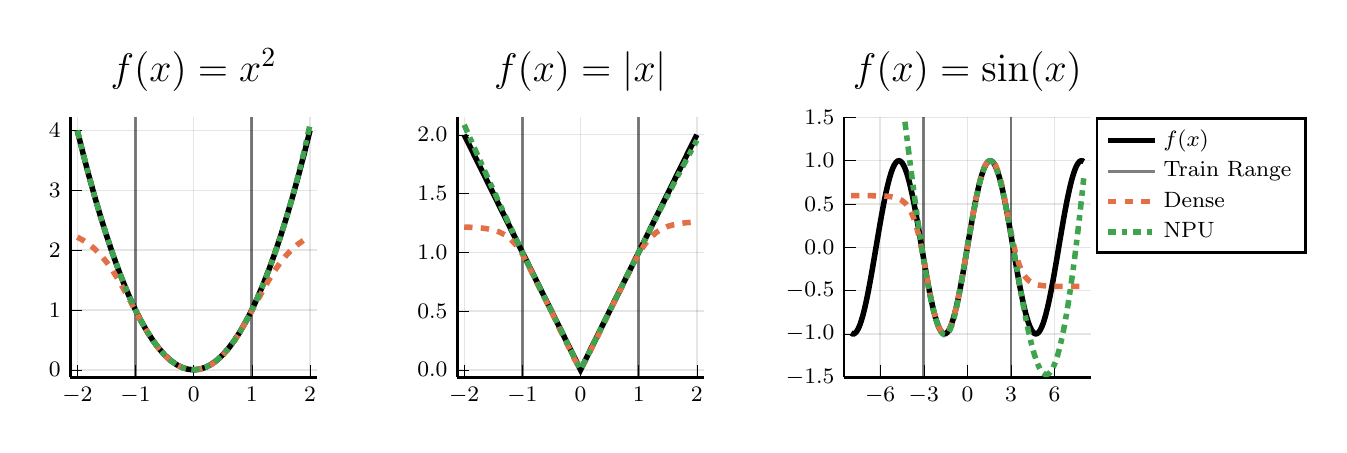
\begin{tikzpicture}[/tikz/background rectangle/.style={fill={rgb,1:red,1.0;green,1.0;blue,1.0}, draw opacity={1.0}}, show background rectangle]
\begin{axis}[point meta max={nan}, point meta min={nan}, legend cell align={left}, title={$f(x) = x^2$}, title style={at={{(0.5,1)}}, anchor={south}, font={{\fontsize{14 pt}{18.2 pt}\selectfont}}, color={rgb,1:red,0.0;green,0.0;blue,0.0}, draw opacity={1.0}, rotate={0.0}}, legend style={color={rgb,1:red,0.0;green,0.0;blue,0.0}, draw opacity={1.0}, line width={1}, solid, fill={rgb,1:red,1.0;green,1.0;blue,1.0}, fill opacity={1.0}, text opacity={1.0}, font={{\fontsize{8 pt}{10.4 pt}\selectfont}}, at={(1.02, 1)}, anchor={north west}}, axis background/.style={fill={rgb,1:red,1.0;green,1.0;blue,1.0}, opacity={1.0}}, anchor={north west}, xshift={1.0mm}, yshift={-1.0mm}, width={47.13333333333333mm}, height={48.8mm}, scaled x ticks={false}, xlabel={}, x tick style={color={rgb,1:red,0.0;green,0.0;blue,0.0}, opacity={1.0}}, x tick label style={color={rgb,1:red,0.0;green,0.0;blue,0.0}, opacity={1.0}, rotate={0}}, xlabel style={at={(ticklabel cs:0.5)}, anchor=near ticklabel, font={{\fontsize{11 pt}{14.3 pt}\selectfont}}, color={rgb,1:red,0.0;green,0.0;blue,0.0}, draw opacity={1.0}, rotate={0.0}}, xmajorgrids={true}, xmin={-2.12}, xmax={2.12}, xtick={{-2.0,-1.0,0.0,1.0,2.0}}, xticklabels={{$-2$,$-1$,$0$,$1$,$2$}}, xtick align={inside}, xticklabel style={font={{\fontsize{8 pt}{10.4 pt}\selectfont}}, color={rgb,1:red,0.0;green,0.0;blue,0.0}, draw opacity={1.0}, rotate={0.0}}, x grid style={color={rgb,1:red,0.0;green,0.0;blue,0.0}, draw opacity={0.1}, line width={0.5}, solid}, axis x line*={left}, x axis line style={color={rgb,1:red,0.0;green,0.0;blue,0.0}, draw opacity={1.0}, line width={1}, solid}, scaled y ticks={false}, ylabel={}, y tick style={color={rgb,1:red,0.0;green,0.0;blue,0.0}, opacity={1.0}}, y tick label style={color={rgb,1:red,0.0;green,0.0;blue,0.0}, opacity={1.0}, rotate={0}}, ylabel style={at={(ticklabel cs:0.5)}, anchor=near ticklabel, font={{\fontsize{11 pt}{14.3 pt}\selectfont}}, color={rgb,1:red,0.0;green,0.0;blue,0.0}, draw opacity={1.0}, rotate={0.0}}, ymajorgrids={true}, ymin={-0.1228785753250122}, ymax={4.218831086158753}, ytick={{0.0,1.0,2.0,3.0,4.0}}, yticklabels={{$0$,$1$,$2$,$3$,$4$}}, ytick align={inside}, yticklabel style={font={{\fontsize{8 pt}{10.4 pt}\selectfont}}, color={rgb,1:red,0.0;green,0.0;blue,0.0}, draw opacity={1.0}, rotate={0.0}}, y grid style={color={rgb,1:red,0.0;green,0.0;blue,0.0}, draw opacity={0.1}, line width={0.5}, solid}, axis y line*={left}, y axis line style={color={rgb,1:red,0.0;green,0.0;blue,0.0}, draw opacity={1.0}, line width={1}, solid}]
    \addplot[color={rgb,1:red,0.0;green,0.0;blue,0.0}, name path={cb8d5ae3-bb1a-4f76-96e1-d8b0b365c2fe}, draw opacity={1.0}, line width={2}, solid]
        table[row sep={\\}]
        {
            \\
            -2.0  4.0  \\
            -1.9  3.61  \\
            -1.8  3.2399998  \\
            -1.7  2.89  \\
            -1.6  2.5600002  \\
            -1.5  2.25  \\
            -1.4  1.9599999  \\
            -1.3  1.6899998  \\
            -1.2  1.44  \\
            -1.1  1.21  \\
            -1.0  1.0  \\
            -0.9  0.80999994  \\
            -0.8  0.64000005  \\
            -0.7  0.48999998  \\
            -0.6  0.36  \\
            -0.5  0.25  \\
            -0.4  0.16000001  \\
            -0.3  0.09  \\
            -0.2  0.040000003  \\
            -0.1  0.010000001  \\
            0.0  0.0  \\
            0.1  0.010000001  \\
            0.2  0.040000003  \\
            0.3  0.09  \\
            0.4  0.16000001  \\
            0.5  0.25  \\
            0.6  0.36  \\
            0.7  0.48999998  \\
            0.8  0.64000005  \\
            0.9  0.80999994  \\
            1.0  1.0  \\
            1.1  1.21  \\
            1.2  1.44  \\
            1.3  1.6899998  \\
            1.4  1.9599999  \\
            1.5  2.25  \\
            1.6  2.5600002  \\
            1.7  2.89  \\
            1.8  3.2399998  \\
            1.9  3.61  \\
            2.0  4.0  \\
        }
        ;
    \addplot[color={rgb,1:red,0.0;green,0.0;blue,0.0}, name path={d996f515-c94c-4145-b670-ad9a0df9e2eb}, draw opacity={0.5}, line width={1}, solid]
        table[row sep={\\}]
        {
            \\
            -1.0  -4.464588236808778  \\
            -1.0  8.560540747642518  \\
        }
        ;
    \addplot[color={rgb,1:red,0.0;green,0.0;blue,0.0}, name path={d996f515-c94c-4145-b670-ad9a0df9e2eb}, draw opacity={0.5}, line width={1}, solid]
        table[row sep={\\}]
        {
            \\
            1.0  -4.464588236808778  \\
            1.0  8.560540747642518  \\
        }
        ;
    \addplot[color={rgb,1:red,0.8889;green,0.4356;blue,0.2781}, name path={c0a19fca-1825-421c-b99e-c4693cccbb01}, draw opacity={1.0}, line width={2}, dashed]
        table[row sep={\\}]
        {
            \\
            -2.0  2.2175353  \\
            -1.9  2.1652787  \\
            -1.8  2.0999224  \\
            -1.7  2.0192063  \\
            -1.6  1.9211061  \\
            -1.5  1.8042185  \\
            -1.4  1.6682322  \\
            -1.3  1.5143886  \\
            -1.2  1.3457947  \\
            -1.1  1.1674106  \\
            -1.0  0.9856209  \\
            -0.9  0.8074259  \\
            -0.8  0.6394708  \\
            -0.7  0.4871961  \\
            -0.6  0.35434574  \\
            -0.5  0.24290484  \\
            -0.4  0.1533894  \\
            -0.3  0.08532515  \\
            -0.2  0.037757277  \\
            -0.1  0.0096870065  \\
            0.0  0.00038653612  \\
            0.1  0.009584248  \\
            0.2  0.037525535  \\
            0.3  0.08491385  \\
            0.4  0.1527282  \\
            0.5  0.24191368  \\
            0.6  0.3529526  \\
            0.7  0.4853617  \\
            0.8  0.63721913  \\
            0.9  0.8048696  \\
            1.0  0.9829703  \\
            1.1  1.1649592  \\
            1.2  1.3438771  \\
            1.3  1.5133243  \\
            1.4  1.6682708  \\
            1.5  1.805506  \\
            1.6  1.9236712  \\
            1.7  2.022975  \\
            1.8  2.1047406  \\
            1.9  2.170942  \\
            2.0  2.2238147  \\
        }
        ;
    \addplot[color={rgb,1:red,0.2422;green,0.6433;blue,0.3044}, name path={5497d2b6-1574-4580-93c5-73bc83e775a5}, draw opacity={1.0}, line width={2}, dashdotted]
        table[row sep={\\}]
        {
            \\
            -2.0  4.002221  \\
            -1.9  3.6118083  \\
            -1.8  3.2414439  \\
            -1.7  2.8911288  \\
            -1.6  2.5608563  \\
            -1.5  2.2506254  \\
            -1.4  1.960433  \\
            -1.3  1.6902772  \\
            -1.2  1.4401559  \\
            -1.1  1.2100648  \\
            -1.0  1.0000015  \\
            -0.9  0.8099637  \\
            -0.8  0.63994837  \\
            -0.7  0.4899512  \\
            -0.6  0.35996866  \\
            -0.5  0.24999587  \\
            -0.4  0.16002735  \\
            -0.3  0.09005613  \\
            -0.2  0.040072832  \\
            -0.1  0.010063502  \\
            0.0  3.3157303e-7  \\
            0.1  0.01003649  \\
            0.2  0.03995353  \\
            0.3  0.08989377  \\
            0.4  0.15996888  \\
            0.5  0.2500343  \\
            0.6  0.3600179  \\
            0.7  0.4899801  \\
            0.8  0.63998413  \\
            0.9  0.81000143  \\
            1.0  0.99990696  \\
            1.1  1.2095305  \\
            1.2  1.4387404  \\
            1.3  1.6875515  \\
            1.4  1.9562633  \\
            1.5  2.245636  \\
            1.6  2.5571256  \\
            1.7  2.8931777  \\
            1.8  3.2575889  \\
            1.9  3.6559207  \\
            2.0  4.0959525  \\
        }
        ;
\end{axis}
\begin{axis}[point meta max={nan}, point meta min={nan}, legend cell align={left}, title={$f(x) = |x|$}, title style={at={{(0.5,1)}}, anchor={south}, font={{\fontsize{14 pt}{18.2 pt}\selectfont}}, color={rgb,1:red,0.0;green,0.0;blue,0.0}, draw opacity={1.0}, rotate={0.0}}, legend style={color={rgb,1:red,0.0;green,0.0;blue,0.0}, draw opacity={1.0}, line width={1}, solid, fill={rgb,1:red,1.0;green,1.0;blue,1.0}, fill opacity={1.0}, text opacity={1.0}, font={{\fontsize{8 pt}{10.4 pt}\selectfont}}, at={(1.02, 1)}, anchor={north west}}, axis background/.style={fill={rgb,1:red,1.0;green,1.0;blue,1.0}, opacity={1.0}}, anchor={north west}, xshift={50.13333333333333mm}, yshift={-1.0mm}, width={47.13333333333333mm}, height={48.8mm}, scaled x ticks={false}, xlabel={}, x tick style={color={rgb,1:red,0.0;green,0.0;blue,0.0}, opacity={1.0}}, x tick label style={color={rgb,1:red,0.0;green,0.0;blue,0.0}, opacity={1.0}, rotate={0}}, xlabel style={at={(ticklabel cs:0.5)}, anchor=near ticklabel, font={{\fontsize{11 pt}{14.3 pt}\selectfont}}, color={rgb,1:red,0.0;green,0.0;blue,0.0}, draw opacity={1.0}, rotate={0.0}}, xmajorgrids={true}, xmin={-2.12}, xmax={2.12}, xtick={{-2.0,-1.0,0.0,1.0,2.0}}, xticklabels={{$-2$,$-1$,$0$,$1$,$2$}}, xtick align={inside}, xticklabel style={font={{\fontsize{8 pt}{10.4 pt}\selectfont}}, color={rgb,1:red,0.0;green,0.0;blue,0.0}, draw opacity={1.0}, rotate={0.0}}, x grid style={color={rgb,1:red,0.0;green,0.0;blue,0.0}, draw opacity={0.1}, line width={0.5}, solid}, axis x line*={left}, x axis line style={color={rgb,1:red,0.0;green,0.0;blue,0.0}, draw opacity={1.0}, line width={1}, solid}, scaled y ticks={false}, ylabel={}, y tick style={color={rgb,1:red,0.0;green,0.0;blue,0.0}, opacity={1.0}}, y tick label style={color={rgb,1:red,0.0;green,0.0;blue,0.0}, opacity={1.0}, rotate={0}}, ylabel style={at={(ticklabel cs:0.5)}, anchor=near ticklabel, font={{\fontsize{11 pt}{14.3 pt}\selectfont}}, color={rgb,1:red,0.0;green,0.0;blue,0.0}, draw opacity={1.0}, rotate={0.0}}, ymajorgrids={true}, ymin={-0.06254863500595093}, ymax={2.1475031352043152}, ytick={{0.0,0.5,1.0,1.5,2.0}}, yticklabels={{$0.0$,$0.5$,$1.0$,$1.5$,$2.0$}}, ytick align={inside}, yticklabel style={font={{\fontsize{8 pt}{10.4 pt}\selectfont}}, color={rgb,1:red,0.0;green,0.0;blue,0.0}, draw opacity={1.0}, rotate={0.0}}, y grid style={color={rgb,1:red,0.0;green,0.0;blue,0.0}, draw opacity={0.1}, line width={0.5}, solid}, axis y line*={left}, y axis line style={color={rgb,1:red,0.0;green,0.0;blue,0.0}, draw opacity={1.0}, line width={1}, solid}]
    \addplot[color={rgb,1:red,0.0;green,0.0;blue,0.0}, name path={d9fa0dbb-8610-41e3-b750-578c3b74e776}, draw opacity={1.0}, line width={2}, solid]
        table[row sep={\\}]
        {
            \\
            -2.0  2.0  \\
            -1.9  1.9  \\
            -1.8  1.8  \\
            -1.7  1.7  \\
            -1.6  1.6  \\
            -1.5  1.5  \\
            -1.4  1.4  \\
            -1.3  1.3  \\
            -1.2  1.2  \\
            -1.1  1.1  \\
            -1.0  1.0  \\
            -0.9  0.9  \\
            -0.8  0.8  \\
            -0.7  0.7  \\
            -0.6  0.6  \\
            -0.5  0.5  \\
            -0.4  0.4  \\
            -0.3  0.3  \\
            -0.2  0.2  \\
            -0.1  0.1  \\
            0.0  0.0  \\
            0.1  0.1  \\
            0.2  0.2  \\
            0.3  0.3  \\
            0.4  0.4  \\
            0.5  0.5  \\
            0.6  0.6  \\
            0.7  0.7  \\
            0.8  0.8  \\
            0.9  0.9  \\
            1.0  1.0  \\
            1.1  1.1  \\
            1.2  1.2  \\
            1.3  1.3  \\
            1.4  1.4  \\
            1.5  1.5  \\
            1.6  1.6  \\
            1.7  1.7  \\
            1.8  1.8  \\
            1.9  1.9  \\
            2.0  2.0  \\
        }
        ;
    \addplot[color={rgb,1:red,0.0;green,0.0;blue,0.0}, name path={6f314365-5491-4c06-b3d6-061baa0fcf69}, draw opacity={0.5}, line width={1}, solid]
        table[row sep={\\}]
        {
            \\
            -1.0  -2.272600405216217  \\
            -1.0  4.357554905414581  \\
        }
        ;
    \addplot[color={rgb,1:red,0.0;green,0.0;blue,0.0}, name path={6f314365-5491-4c06-b3d6-061baa0fcf69}, draw opacity={0.5}, line width={1}, solid]
        table[row sep={\\}]
        {
            \\
            1.0  -2.272600405216217  \\
            1.0  4.357554905414581  \\
        }
        ;
    \addplot[color={rgb,1:red,0.8889;green,0.4356;blue,0.2781}, name path={25ca6b39-6927-49ca-95ef-9a43c14fdcee}, draw opacity={1.0}, line width={2}, dashed]
        table[row sep={\\}]
        {
            \\
            -2.0  1.2146502  \\
            -1.9  1.2130404  \\
            -1.8  1.210468  \\
            -1.7  1.2063661  \\
            -1.6  1.1998477  \\
            -1.5  1.1895502  \\
            -1.4  1.1734347  \\
            -1.3  1.1486006  \\
            -1.2  1.1112721  \\
            -1.1  1.0573483  \\
            -1.0  0.98409617  \\
            -0.9  0.89305735  \\
            -0.8  0.79193693  \\
            -0.7  0.6909176  \\
            -0.6  0.5938499  \\
            -0.5  0.49543518  \\
            -0.4  0.39129728  \\
            -0.3  0.28711027  \\
            -0.2  0.18959016  \\
            -0.1  0.08753854  \\
            0.0  0.0072743893  \\
            0.1  0.08825743  \\
            0.2  0.19297999  \\
            0.3  0.2902612  \\
            0.4  0.3930353  \\
            0.5  0.4960415  \\
            0.6  0.59480476  \\
            0.7  0.69244325  \\
            0.8  0.7929653  \\
            0.9  0.89370286  \\
            1.0  0.98654616  \\
            1.1  1.0643454  \\
            1.2  1.1245524  \\
            1.3  1.16854  \\
            1.4  1.1994584  \\
            1.5  1.2206502  \\
            1.6  1.2349424  \\
            1.7  1.2444816  \\
            1.8  1.2508059  \\
            1.9  1.2549806  \\
            2.0  1.2577289  \\
        }
        ;
    \addplot[color={rgb,1:red,0.2422;green,0.6433;blue,0.3044}, name path={e673a053-60ec-403b-b123-1cb79eec1eec}, draw opacity={1.0}, line width={2}, dashdotted]
        table[row sep={\\}]
        {
            \\
            -2.0  2.0849545  \\
            -1.9  1.9720565  \\
            -1.8  1.8601044  \\
            -1.7  1.749136  \\
            -1.6  1.6391871  \\
            -1.5  1.5302888  \\
            -1.4  1.4224697  \\
            -1.3  1.3157496  \\
            -1.2  1.210142  \\
            -1.1  1.1056455  \\
            -1.0  1.0022453  \\
            -0.9  0.8999029  \\
            -0.8  0.7985524  \\
            -0.7  0.69808894  \\
            -0.6  0.5983573  \\
            -0.5  0.4991328  \\
            -0.4  0.4000996  \\
            -0.3  0.30081475  \\
            -0.2  0.2006641  \\
            -0.1  0.0987964  \\
            0.0  0.0011098385  \\
            0.1  0.1006847  \\
            0.2  0.20042723  \\
            0.3  0.30037892  \\
            0.4  0.40050787  \\
            0.5  0.5007406  \\
            0.6  0.6009805  \\
            0.7  0.7011212  \\
            0.8  0.80105436  \\
            0.9  0.90067387  \\
            1.0  0.99987984  \\
            1.1  1.0985794  \\
            1.2  1.1966882  \\
            1.3  1.2941289  \\
            1.4  1.3908343  \\
            1.5  1.4867432  \\
            1.6  1.5818037  \\
            1.7  1.6759676  \\
            1.8  1.769196  \\
            1.9  1.8614548  \\
            2.0  1.9527144  \\
        }
        ;
\end{axis}
\begin{axis}[point meta max={nan}, point meta min={nan}, legend cell align={left}, title={$f(x) = \sin(x)$}, title style={at={{(0.5,1)}}, anchor={south}, font={{\fontsize{14 pt}{18.2 pt}\selectfont}}, color={rgb,1:red,0.0;green,0.0;blue,0.0}, draw opacity={1.0}, rotate={0.0}}, legend style={color={rgb,1:red,0.0;green,0.0;blue,0.0}, draw opacity={1.0}, line width={1}, solid, fill={rgb,1:red,1.0;green,1.0;blue,1.0}, fill opacity={1.0}, text opacity={1.0}, font={{\fontsize{8 pt}{10.4 pt}\selectfont}}, at={(1.02, 1)}, anchor={north west}}, axis background/.style={fill={rgb,1:red,1.0;green,1.0;blue,1.0}, opacity={1.0}}, anchor={north west}, xshift={99.26666666666667mm}, yshift={-1.0mm}, width={47.13333333333333mm}, height={48.8mm}, scaled x ticks={false}, xlabel={}, x tick style={color={rgb,1:red,0.0;green,0.0;blue,0.0}, opacity={1.0}}, x tick label style={color={rgb,1:red,0.0;green,0.0;blue,0.0}, opacity={1.0}, rotate={0}}, xlabel style={at={(ticklabel cs:0.5)}, anchor=near ticklabel, font={{\fontsize{11 pt}{14.3 pt}\selectfont}}, color={rgb,1:red,0.0;green,0.0;blue,0.0}, draw opacity={1.0}, rotate={0.0}}, xmajorgrids={true}, xmin={-8.48}, xmax={8.48}, xtick={{-6.0,-3.0,0.0,3.0,6.0}}, xticklabels={{$-6$,$-3$,$0$,$3$,$6$}}, xtick align={inside}, xticklabel style={font={{\fontsize{8 pt}{10.4 pt}\selectfont}}, color={rgb,1:red,0.0;green,0.0;blue,0.0}, draw opacity={1.0}, rotate={0.0}}, x grid style={color={rgb,1:red,0.0;green,0.0;blue,0.0}, draw opacity={0.1}, line width={0.5}, solid}, axis x line*={left}, x axis line style={color={rgb,1:red,0.0;green,0.0;blue,0.0}, draw opacity={1.0}, line width={1}, solid}, scaled y ticks={false}, ylabel={}, y tick style={color={rgb,1:red,0.0;green,0.0;blue,0.0}, opacity={1.0}}, y tick label style={color={rgb,1:red,0.0;green,0.0;blue,0.0}, opacity={1.0}, rotate={0}}, ylabel style={at={(ticklabel cs:0.5)}, anchor=near ticklabel, font={{\fontsize{11 pt}{14.3 pt}\selectfont}}, color={rgb,1:red,0.0;green,0.0;blue,0.0}, draw opacity={1.0}, rotate={0.0}}, ymajorgrids={true}, ymin={-1.5}, ymax={1.5}, ytick={{-1.5,-1.0,-0.5,0.0,0.5,1.0,1.5}}, yticklabels={{$-1.5$,$-1.0$,$-0.5$,$0.0$,$0.5$,$1.0$,$1.5$}}, ytick align={inside}, yticklabel style={font={{\fontsize{8 pt}{10.4 pt}\selectfont}}, color={rgb,1:red,0.0;green,0.0;blue,0.0}, draw opacity={1.0}, rotate={0.0}}, y grid style={color={rgb,1:red,0.0;green,0.0;blue,0.0}, draw opacity={0.1}, line width={0.5}, solid}, axis y line*={left}, y axis line style={color={rgb,1:red,0.0;green,0.0;blue,0.0}, draw opacity={1.0}, line width={1}, solid}]
    \addplot[color={rgb,1:red,0.0;green,0.0;blue,0.0}, name path={09cd4ea2-8a4b-453e-96af-d61364e007a1}, draw opacity={1.0}, line width={2}, solid]
        table[row sep={\\}]
        {
            \\
            -8.0  -0.98935825  \\
            -7.9  -0.99894136  \\
            -7.8  -0.9985434  \\
            -7.7  -0.9881682  \\
            -7.6  -0.96791965  \\
            -7.5  -0.93799996  \\
            -7.4  -0.89870816  \\
            -7.3  -0.85043675  \\
            -7.2  -0.79366773  \\
            -7.1  -0.728969  \\
            -7.0  -0.6569866  \\
            -6.9  -0.57843983  \\
            -6.8  -0.4941135  \\
            -6.7  -0.40484974  \\
            -6.6  -0.31154126  \\
            -6.5  -0.21511999  \\
            -6.4  -0.1165493  \\
            -6.3  -0.01681409  \\
            -6.2  0.08308959  \\
            -6.1  0.1821626  \\
            -6.0  0.2794155  \\
            -5.9  0.37387657  \\
            -5.8  0.46460202  \\
            -5.7  0.5506857  \\
            -5.6  0.6312667  \\
            -5.5  0.7055403  \\
            -5.4  0.77276444  \\
            -5.3  0.83226734  \\
            -5.2  0.88345474  \\
            -5.1  0.92581475  \\
            -5.0  0.9589243  \\
            -4.9  0.9824526  \\
            -4.8  0.9961646  \\
            -4.7  0.9999232  \\
            -4.6  0.99369097  \\
            -4.5  0.9775301  \\
            -4.4  0.9516021  \\
            -4.3  0.916166  \\
            -4.2  0.87157565  \\
            -4.1  0.81827706  \\
            -4.0  0.7568025  \\
            -3.9  0.68776625  \\
            -3.8  0.61185783  \\
            -3.7  0.5298362  \\
            -3.6  0.44252035  \\
            -3.5  0.35078323  \\
            -3.4  0.2555412  \\
            -3.3  0.15774564  \\
            -3.2  0.058374193  \\
            -3.1  -0.04158076  \\
            -3.0  -0.14112  \\
            -2.9  -0.23924923  \\
            -2.8  -0.3349882  \\
            -2.7  -0.42737985  \\
            -2.6  -0.51550144  \\
            -2.5  -0.5984721  \\
            -2.4  -0.67546314  \\
            -2.3  -0.74570525  \\
            -2.2  -0.80849636  \\
            -2.1  -0.8632094  \\
            -2.0  -0.9092974  \\
            -1.9  -0.9463001  \\
            -1.8  -0.9738476  \\
            -1.7  -0.9916648  \\
            -1.6  -0.9995736  \\
            -1.5  -0.997495  \\
            -1.4  -0.98544973  \\
            -1.3  -0.9635582  \\
            -1.2  -0.9320391  \\
            -1.1  -0.8912074  \\
            -1.0  -0.84147096  \\
            -0.9  -0.7833269  \\
            -0.8  -0.7173561  \\
            -0.7  -0.64421767  \\
            -0.6  -0.5646425  \\
            -0.5  -0.47942555  \\
            -0.4  -0.38941833  \\
            -0.3  -0.29552022  \\
            -0.2  -0.19866933  \\
            -0.1  -0.09983342  \\
            0.0  0.0  \\
            0.1  0.09983342  \\
            0.2  0.19866933  \\
            0.3  0.29552022  \\
            0.4  0.38941833  \\
            0.5  0.47942555  \\
            0.6  0.5646425  \\
            0.7  0.64421767  \\
            0.8  0.7173561  \\
            0.9  0.7833269  \\
            1.0  0.84147096  \\
            1.1  0.8912074  \\
            1.2  0.9320391  \\
            1.3  0.9635582  \\
            1.4  0.98544973  \\
            1.5  0.997495  \\
            1.6  0.9995736  \\
            1.7  0.9916648  \\
            1.8  0.9738476  \\
            1.9  0.9463001  \\
            2.0  0.9092974  \\
            2.1  0.8632094  \\
            2.2  0.80849636  \\
            2.3  0.74570525  \\
            2.4  0.67546314  \\
            2.5  0.5984721  \\
            2.6  0.51550144  \\
            2.7  0.42737985  \\
            2.8  0.3349882  \\
            2.9  0.23924923  \\
            3.0  0.14112  \\
            3.1  0.04158076  \\
            3.2  -0.058374193  \\
            3.3  -0.15774564  \\
            3.4  -0.2555412  \\
            3.5  -0.35078323  \\
            3.6  -0.44252035  \\
            3.7  -0.5298362  \\
            3.8  -0.61185783  \\
            3.9  -0.68776625  \\
            4.0  -0.7568025  \\
            4.1  -0.81827706  \\
            4.2  -0.87157565  \\
            4.3  -0.916166  \\
            4.4  -0.9516021  \\
            4.5  -0.9775301  \\
            4.6  -0.99369097  \\
            4.7  -0.9999232  \\
            4.8  -0.9961646  \\
            4.9  -0.9824526  \\
            5.0  -0.9589243  \\
            5.1  -0.92581475  \\
            5.2  -0.88345474  \\
            5.3  -0.83226734  \\
            5.4  -0.77276444  \\
            5.5  -0.7055403  \\
            5.6  -0.6312667  \\
            5.7  -0.5506857  \\
            5.8  -0.46460202  \\
            5.9  -0.37387657  \\
            6.0  -0.2794155  \\
            6.1  -0.1821626  \\
            6.2  -0.08308959  \\
            6.3  0.01681409  \\
            6.4  0.1165493  \\
            6.5  0.21511999  \\
            6.6  0.31154126  \\
            6.7  0.40484974  \\
            6.8  0.4941135  \\
            6.9  0.57843983  \\
            7.0  0.6569866  \\
            7.1  0.728969  \\
            7.2  0.79366773  \\
            7.3  0.85043675  \\
            7.4  0.89870816  \\
            7.5  0.93799996  \\
            7.6  0.96791965  \\
            7.7  0.9881682  \\
            7.8  0.9985434  \\
            7.9  0.99894136  \\
            8.0  0.98935825  \\
        }
        ;
    \addlegendentry {$f(x)$}
    \addplot[color={rgb,1:red,0.0;green,0.0;blue,0.0}, name path={b46d8aad-403e-429a-a943-a94ca1481de0}, draw opacity={0.5}, line width={1}, solid]
        table[row sep={\\}]
        {
            \\
            -3.0  -4.5  \\
            -3.0  4.5  \\
        }
        ;
    \addlegendentry {Train Range}
    \addplot[color={rgb,1:red,0.0;green,0.0;blue,0.0}, name path={b46d8aad-403e-429a-a943-a94ca1481de0}, draw opacity={0.5}, line width={1}, solid, forget plot]
        table[row sep={\\}]
        {
            \\
            3.0  -4.5  \\
            3.0  4.5  \\
        }
        ;
    \addplot[color={rgb,1:red,0.8889;green,0.4356;blue,0.2781}, name path={cac92316-f1f4-488d-9994-a72644230829}, draw opacity={1.0}, line width={2}, dashed]
        table[row sep={\\}]
        {
            \\
            -8.0  0.59659517  \\
            -7.9  0.596581  \\
            -7.8  0.596564  \\
            -7.7  0.59654456  \\
            -7.6  0.5965215  \\
            -7.5  0.5964941  \\
            -7.4  0.5964614  \\
            -7.3  0.5964223  \\
            -7.2  0.59637535  \\
            -7.1  0.5963181  \\
            -7.0  0.59624964  \\
            -6.9  0.5961662  \\
            -6.8  0.5960647  \\
            -6.7  0.595941  \\
            -6.6  0.5957904  \\
            -6.5  0.5956066  \\
            -6.4  0.5953819  \\
            -6.3  0.59510714  \\
            -6.2  0.5947711  \\
            -6.1  0.5943599  \\
            -6.0  0.5938562  \\
            -5.9  0.5932397  \\
            -5.8  0.5924847  \\
            -5.7  0.59156  \\
            -5.6  0.5904274  \\
            -5.5  0.58904105  \\
            -5.4  0.58734334  \\
            -5.3  0.5852656  \\
            -5.2  0.58272314  \\
            -5.1  0.5796146  \\
            -5.0  0.5758156  \\
            -4.9  0.57117665  \\
            -4.8  0.565518  \\
            -4.7  0.55862385  \\
            -4.6  0.55023724  \\
            -4.5  0.5400544  \\
            -4.4  0.52771825  \\
            -4.3  0.5128149  \\
            -4.2  0.4948699  \\
            -4.1  0.47334963  \\
            -4.0  0.44766593  \\
            -3.9  0.4171893  \\
            -3.8  0.38127244  \\
            -3.7  0.33928406  \\
            -3.6  0.29065967  \\
            -3.5  0.23496282  \\
            -3.4  0.17196107  \\
            -3.3  0.101702034  \\
            -3.2  0.024585396  \\
            -3.1  -0.058588  \\
            -3.0  -0.14660569  \\
            -2.9  -0.23788044  \\
            -2.8  -0.33053997  \\
            -2.7  -0.42255569  \\
            -2.6  -0.5119002  \\
            -2.5  -0.5966941  \\
            -2.4  -0.67532897  \\
            -2.3  -0.74653774  \\
            -2.2  -0.8094161  \\
            -2.1  -0.86339515  \\
            -2.0  -0.9081774  \\
            -1.9  -0.9436578  \\
            -1.8  -0.9698417  \\
            -1.7  -0.9867698  \\
            -1.6  -0.99446404  \\
            -1.5  -0.9928944  \\
            -1.4  -0.98197407  \\
            -1.3  -0.96157867  \\
            -1.2  -0.931595  \\
            -1.1  -0.89198667  \\
            -1.0  -0.842872  \\
            -0.9  -0.784594  \\
            -0.8  -0.717765  \\
            -0.7  -0.64326483  \\
            -0.6  -0.56218743  \\
            -0.5  -0.47573742  \\
            -0.4  -0.38510826  \\
            -0.3  -0.2913712  \\
            -0.2  -0.19541232  \\
            -0.1  -0.09793568  \\
            0.0  0.00047315657  \\
            0.1  0.099242836  \\
            0.2  0.19770825  \\
            0.3  0.29503143  \\
            0.4  0.39017475  \\
            0.5  0.48193574  \\
            0.6  0.5690304  \\
            0.7  0.6502043  \\
            0.8  0.72433996  \\
            0.9  0.7905383  \\
            1.0  0.8481573  \\
            1.1  0.89680564  \\
            1.2  0.9363034  \\
            1.3  0.9666183  \\
            1.4  0.987797  \\
            1.5  0.9999006  \\
            1.6  1.002955  \\
            1.7  0.99692154  \\
            1.8  0.98169136  \\
            1.9  0.95710564  \\
            2.0  0.9230025  \\
            2.1  0.8792887  \\
            2.2  0.8260288  \\
            2.3  0.76355016  \\
            2.4  0.69253194  \\
            2.5  0.6140735  \\
            2.6  0.5297091  \\
            2.7  0.4413551  \\
            2.8  0.3511932  \\
            2.9  0.26149416  \\
            3.0  0.1744262  \\
            3.1  0.09187305  \\
            3.2  0.015303493  \\
            3.3  -0.054292202  \\
            3.4  -0.11640191  \\
            3.5  -0.17093503  \\
            3.6  -0.21813786  \\
            3.7  -0.2584952  \\
            3.8  -0.29263854  \\
            3.9  -0.32126808  \\
            4.0  -0.34509623  \\
            4.1  -0.36480546  \\
            4.2  -0.38102412  \\
            4.3  -0.3943143  \\
            4.4  -0.4051671  \\
            4.5  -0.41400468  \\
            4.6  -0.4211849  \\
            4.7  -0.42700768  \\
            4.8  -0.43172228  \\
            4.9  -0.43553543  \\
            5.0  -0.43861663  \\
            5.1  -0.44110394  \\
            5.2  -0.4431113  \\
            5.3  -0.4447304  \\
            5.4  -0.4460354  \\
            5.5  -0.44708753  \\
            5.6  -0.44793522  \\
            5.7  -0.4486189  \\
            5.8  -0.44916975  \\
            5.9  -0.44961345  \\
            6.0  -0.44997156  \\
            6.1  -0.45025992  \\
            6.2  -0.45049262  \\
            6.3  -0.4506806  \\
            6.4  -0.4508325  \\
            6.5  -0.4509549  \\
            6.6  -0.4510541  \\
            6.7  -0.45113468  \\
            6.8  -0.4512  \\
            6.9  -0.45125294  \\
            7.0  -0.4512961  \\
            7.1  -0.4513315  \\
            7.2  -0.45136058  \\
            7.3  -0.45138443  \\
            7.4  -0.4514042  \\
            7.5  -0.45142066  \\
            7.6  -0.45143437  \\
            7.7  -0.45144618  \\
            7.8  -0.45145607  \\
            7.9  -0.45146453  \\
            8.0  -0.45147192  \\
        }
        ;
    \addlegendentry {Dense}
    \addplot[color={rgb,1:red,0.2422;green,0.6433;blue,0.3044}, name path={1270500e-5b3c-403c-8a9c-91e018368c08}, draw opacity={1.0}, line width={2}, dashdotted]
        table[row sep={\\}]
        {
            \\
            -8.0  6.010978  \\
            -7.9  5.915226  \\
            -7.8  5.817529  \\
            -7.7  5.7178974  \\
            -7.6  5.6163483  \\
            -7.5  5.5128975  \\
            -7.4  5.4075594  \\
            -7.3  5.3003554  \\
            -7.2  5.1913104  \\
            -7.1  5.080448  \\
            -7.0  4.967796  \\
            -6.9  4.8533874  \\
            -6.8  4.7372546  \\
            -6.7  4.6194324  \\
            -6.6  4.499963  \\
            -6.5  4.3788896  \\
            -6.4  4.256258  \\
            -6.3  4.132122  \\
            -6.2  4.0065336  \\
            -6.1  3.8795538  \\
            -6.0  3.7512445  \\
            -5.9  3.621674  \\
            -5.8  3.4909163  \\
            -5.7  3.3590474  \\
            -5.6  3.2261512  \\
            -5.5  3.0923173  \\
            -5.4  2.9576383  \\
            -5.3  2.8222156  \\
            -5.2  2.6861548  \\
            -5.1  2.549571  \\
            -5.0  2.4125848  \\
            -4.9  2.2753227  \\
            -4.8  2.1379197  \\
            -4.7  2.0005183  \\
            -4.6  1.8632718  \\
            -4.5  1.7263393  \\
            -4.4  1.5898892  \\
            -4.3  1.4541004  \\
            -4.2  1.3191592  \\
            -4.1  1.1852655  \\
            -4.0  1.0526266  \\
            -3.9  0.9214608  \\
            -3.8  0.7920008  \\
            -3.7  0.66448474  \\
            -3.6  0.5391677  \\
            -3.5  0.41631633  \\
            -3.4  0.29620516  \\
            -3.3  0.17912793  \\
            -3.2  0.065384865  \\
            -3.1  -0.044706583  \\
            -3.0  -0.15081918  \\
            -2.9  -0.25261182  \\
            -2.8  -0.3497312  \\
            -2.7  -0.44181216  \\
            -2.6  -0.528478  \\
            -2.5  -0.60934204  \\
            -2.4  -0.68401  \\
            -2.3  -0.75207883  \\
            -2.2  -0.81313974  \\
            -2.1  -0.8667824  \\
            -2.0  -0.9125969  \\
            -1.9  -0.95017934  \\
            -1.8  -0.97913384  \\
            -1.7  -0.999084  \\
            -1.6  -1.0096785  \\
            -1.5  -1.0105984  \\
            -1.4  -1.0015744  \\
            -1.3  -0.9823978  \\
            -1.2  -0.9529427  \\
            -1.1  -0.9131857  \\
            -1.0  -0.8632354  \\
            -0.9  -0.80336857  \\
            -0.8  -0.7340719  \\
            -0.7  -0.656093  \\
            -0.6  -0.5705137  \\
            -0.5  -0.47882432  \\
            -0.4  -0.38303426  \\
            -0.3  -0.28579828  \\
            -0.2  -0.190582  \\
            -0.1  -0.101870045  \\
            0.0  0.024224237  \\
            0.1  0.10692157  \\
            0.2  0.19462949  \\
            0.3  0.28515452  \\
            0.4  0.37638572  \\
            0.5  0.46634504  \\
            0.6  0.5532244  \\
            0.7  0.63540864  \\
            0.8  0.71148944  \\
            0.9  0.780269  \\
            1.0  0.84075946  \\
            1.1  0.8921756  \\
            1.2  0.9339248  \\
            1.3  0.96559507  \\
            1.4  0.9869408  \\
            1.5  0.9978676  \\
            1.6  0.9984182  \\
            1.7  0.9887565  \\
            1.8  0.96915376  \\
            1.9  0.9399736  \\
            2.0  0.90165997  \\
            2.1  0.85472274  \\
            2.2  0.7997292  \\
            2.3  0.73729104  \\
            2.4  0.66805434  \\
            2.5  0.59269273  \\
            2.6  0.5118971  \\
            2.7  0.42637062  \\
            2.8  0.3368209  \\
            2.9  0.24395485  \\
            3.0  0.14847273  \\
            3.1  0.051066548  \\
            3.2  -0.047588944  \\
            3.3  -0.14683318  \\
            3.4  -0.24602652  \\
            3.5  -0.34455353  \\
            3.6  -0.4418199  \\
            3.7  -0.5372603  \\
            3.8  -0.6303344  \\
            3.9  -0.72053057  \\
            4.0  -0.80736697  \\
            4.1  -0.8903892  \\
            4.2  -0.9691738  \\
            4.3  -1.0433261  \\
            4.4  -1.1124802  \\
            4.5  -1.1763012  \\
            4.6  -1.2344819  \\
            4.7  -1.2867434  \\
            4.8  -1.3328351  \\
            4.9  -1.3725322  \\
            5.0  -1.4056377  \\
            5.1  -1.4319816  \\
            5.2  -1.4514155  \\
            5.3  -1.4638176  \\
            5.4  -1.4690877  \\
            5.5  -1.4671495  \\
            5.6  -1.4579475  \\
            5.7  -1.4414468  \\
            5.8  -1.4176304  \\
            5.9  -1.3865038  \\
            6.0  -1.3480868  \\
            6.1  -1.3024173  \\
            6.2  -1.2495501  \\
            6.3  -1.1895536  \\
            6.4  -1.1225122  \\
            6.5  -1.0485221  \\
            6.6  -0.9676949  \\
            6.7  -0.8801496  \\
            6.8  -0.7860197  \\
            6.9  -0.68544996  \\
            7.0  -0.5785893  \\
            7.1  -0.46560213  \\
            7.2  -0.34665856  \\
            7.3  -0.22193336  \\
            7.4  -0.0916107  \\
            7.5  0.044117242  \\
            7.6  0.18505529  \\
            7.7  0.33100212  \\
            7.8  0.48175544  \\
            7.9  0.6371002  \\
            8.0  0.79682493  \\
        }
        ;
    \addlegendentry {NPU}
\end{axis}
\end{tikzpicture}
}
\end{frame}

\begin{frame}{Inductive Bias}
  \begin{enumerate}
    \item Assume \textbf{composition} of arithmetic operations.
    \item Construct layers with \textbf{inductive bias} towards arithmetic operations.
  \end{enumerate}
  \vfill

  \begin{columns}[t]
    \column{.5\textwidth}\centering
    \textbf{Addition} of inputs
    \begin{equation*}
      \phantom{\prod_i}\bm x^\intercal \bm w = x_1w_1 + x_2w_2 + \dots
    \end{equation*}
    is simple.

    \column{.5\textwidth}\centering
    \textbf{Multiplication}/\textbf{power functions}
    \begin{equation*}
      \prod_i x_i^{w_i} = \exp(\bm w^\intercal \log \bm x)
    \end{equation*}
    a bit more tricky due to complex outputs...

  \end{columns}
\end{frame}

\begin{frame}{Neural Arithmetic Logic Unit (NALU)}
  \begin{columns}
    \column{.5\textwidth}
      % \documentclass[tikz,14pt,border=10pt]{standalone}
% 
% \usepackage{verbatim}
% \usepackage{bm}
% 
% \usetikzlibrary{%
%   arrows,%
%   shapes.misc,% wg. rounded rectangle
%   shapes.arrows,%
%   chains,%
%   matrix,%
%   positioning,% wg. " of "
%   scopes,%
%   decorations.pathmorphing,% /pgf/decoration/random steps | erste Graphik
%   shadows%
% }
% \begin{document}

\definecolor{c1}{HTML}{8097e9}
\definecolor{c2}{HTML}{c6dea2}
\definecolor{c3}{HTML}{ffb200}
\definecolor{c4}{HTML}{b6b6b6}

\tikzset{
  function/.style={
    % The shape:
    rectangle,
    rounded corners=3,
    % The size:
    minimum height=6mm,
    % The border:
    thick,
    draw=black,
    % The filling:
    top color=c1,
    bottom color=c1,
    % Font
    font=\tt
  },
  vector/.style={
    % The shape:
    rounded rectangle,
    minimum size=6mm,
    % The rest
    thick,draw=black,
    top color=c2!80,
    bottom color=c2!80,
    font=\ttfamily
  },
  trainable/.style={
    % The shape:
    diamond,
    rounded corners=3,
    minimum size=6mm,
    % The rest
    thick,draw=black,
    top color=c3!80,
    bottom color=c3!80,
    font=\ttfamily
  },
  skip loop/.style={to path={-- ++(0,#1) -| (\tikztotarget)}}
}

{
  \tikzset{vector/.append style={text height=1.5ex,text depth=.25ex}}
  \tikzset{function/.append style={text height=1.5ex,text depth=.25ex}}
}

\begin{tikzpicture}[
        point/.style={coordinate},>=stealth',thick,draw=black!90,
        tip/.style={->,shorten >=0.007pt},every join/.style={rounded corners},
        fat/.style={-, ultra thick, opacity=0.5},every join/.style={rounded corners},
        hv path/.style={to path={-| (\tikztotarget)}},
        vh path/.style={to path={|- (\tikztotarget)}},
        path/.style={to path={-- (\tikztotarget)}},
        text height=1.5ex,text depth=.25ex]

  \matrix[column sep=3mm, row sep=1mm] {
    & & \node (add) [function] {$\mathrm{add}$}; &
    \node (a) [vector] {$\bm a$}; \\

    \node (x) [vector] {$\bm x$}; &
    \node (W) [trainable] {$\bm W$}; &
    \node (tanhs) [function] {$\mathrm{tanh}\sigma$};&
    \node (g) [trainable] {$\bm g$}; & &
    \node (gate) [function] {$\mathrm{gate}$}; & &
    \node (y) [vector] {$\bm y$};\\
    
    & \node (M) [trainable] {$\bm M$}; &\\

    & & \node (mult) [function] {$\mathrm{mult}$}; &
    \node (m) [vector] {$\bm m$}; \\
  };

  { [start chain]
    \chainin (x);
    \chainin (mult) [join=by {vh path, tip}];
    \chainin (m) [join=by path];
    \chainin (gate) [join=by {hv path, tip}];
  }

  { [start chain]
    \chainin (x);
    \chainin (add) [join=by {vh path, tip}];
    \chainin (a) [join=by path];
    \chainin (gate) [join=by {hv path, tip}];
    \chainin (y) [join=by {tip}];
  }

  { [start chain]
    \chainin (W);
    \chainin (tanhs) [join=by tip];
    \chainin (add) [join=by tip];
  }
  { [start chain]
    \chainin (M);
    \chainin (tanhs) [join=by tip];
    \chainin (mult) [join=by tip];
  }
  { [start chain]
    \chainin (g);
    \chainin (gate) [join=by tip];
  }



\end{tikzpicture}

% \end{document}


    \column{.5\textwidth}
      \begin{align*}
        \add(\bm x, \hat{\bm W}) &= \hat{\bm W} \bm x \\
        \mult(\bm x, \hat{\bm W}) &= \exp(\hat{\bm W} \log |\bm x|+\epsilon) \\
        \gate(\bm a, \bm m, \bm g) &= \bm g \odot \bm a + (1-\bm g) \odot \bm m \\
        \tanhs(\bm W, \bm M) &= \tanh(\bm W)\odot\sigma(\bm M)
      \end{align*}
      \begin{center}where\end{center}
      \begin{align*}
        \bm g = \sigma(\bm G \bm x)
      \end{align*}
  \end{columns}

  \vfill
  {\tiny(\emph{Neural Arithmetic Logic Units}  - Trask et al. 2018)}
\end{frame}

\begin{frame}
  \begin{columns}
    \column{.35\textwidth}\centering
    Task: Learn $f$ in \emph{one} model
    \begin{equation*}
      f(x,y) = (x+y, xy, \frac{x}{y}, \sqrt{y})^\intercal
    \end{equation*}

    \column{.65\textwidth}
    \begin{tikzpicture}
      \node[anchor=south west, inner sep=0] at (0,0) {
        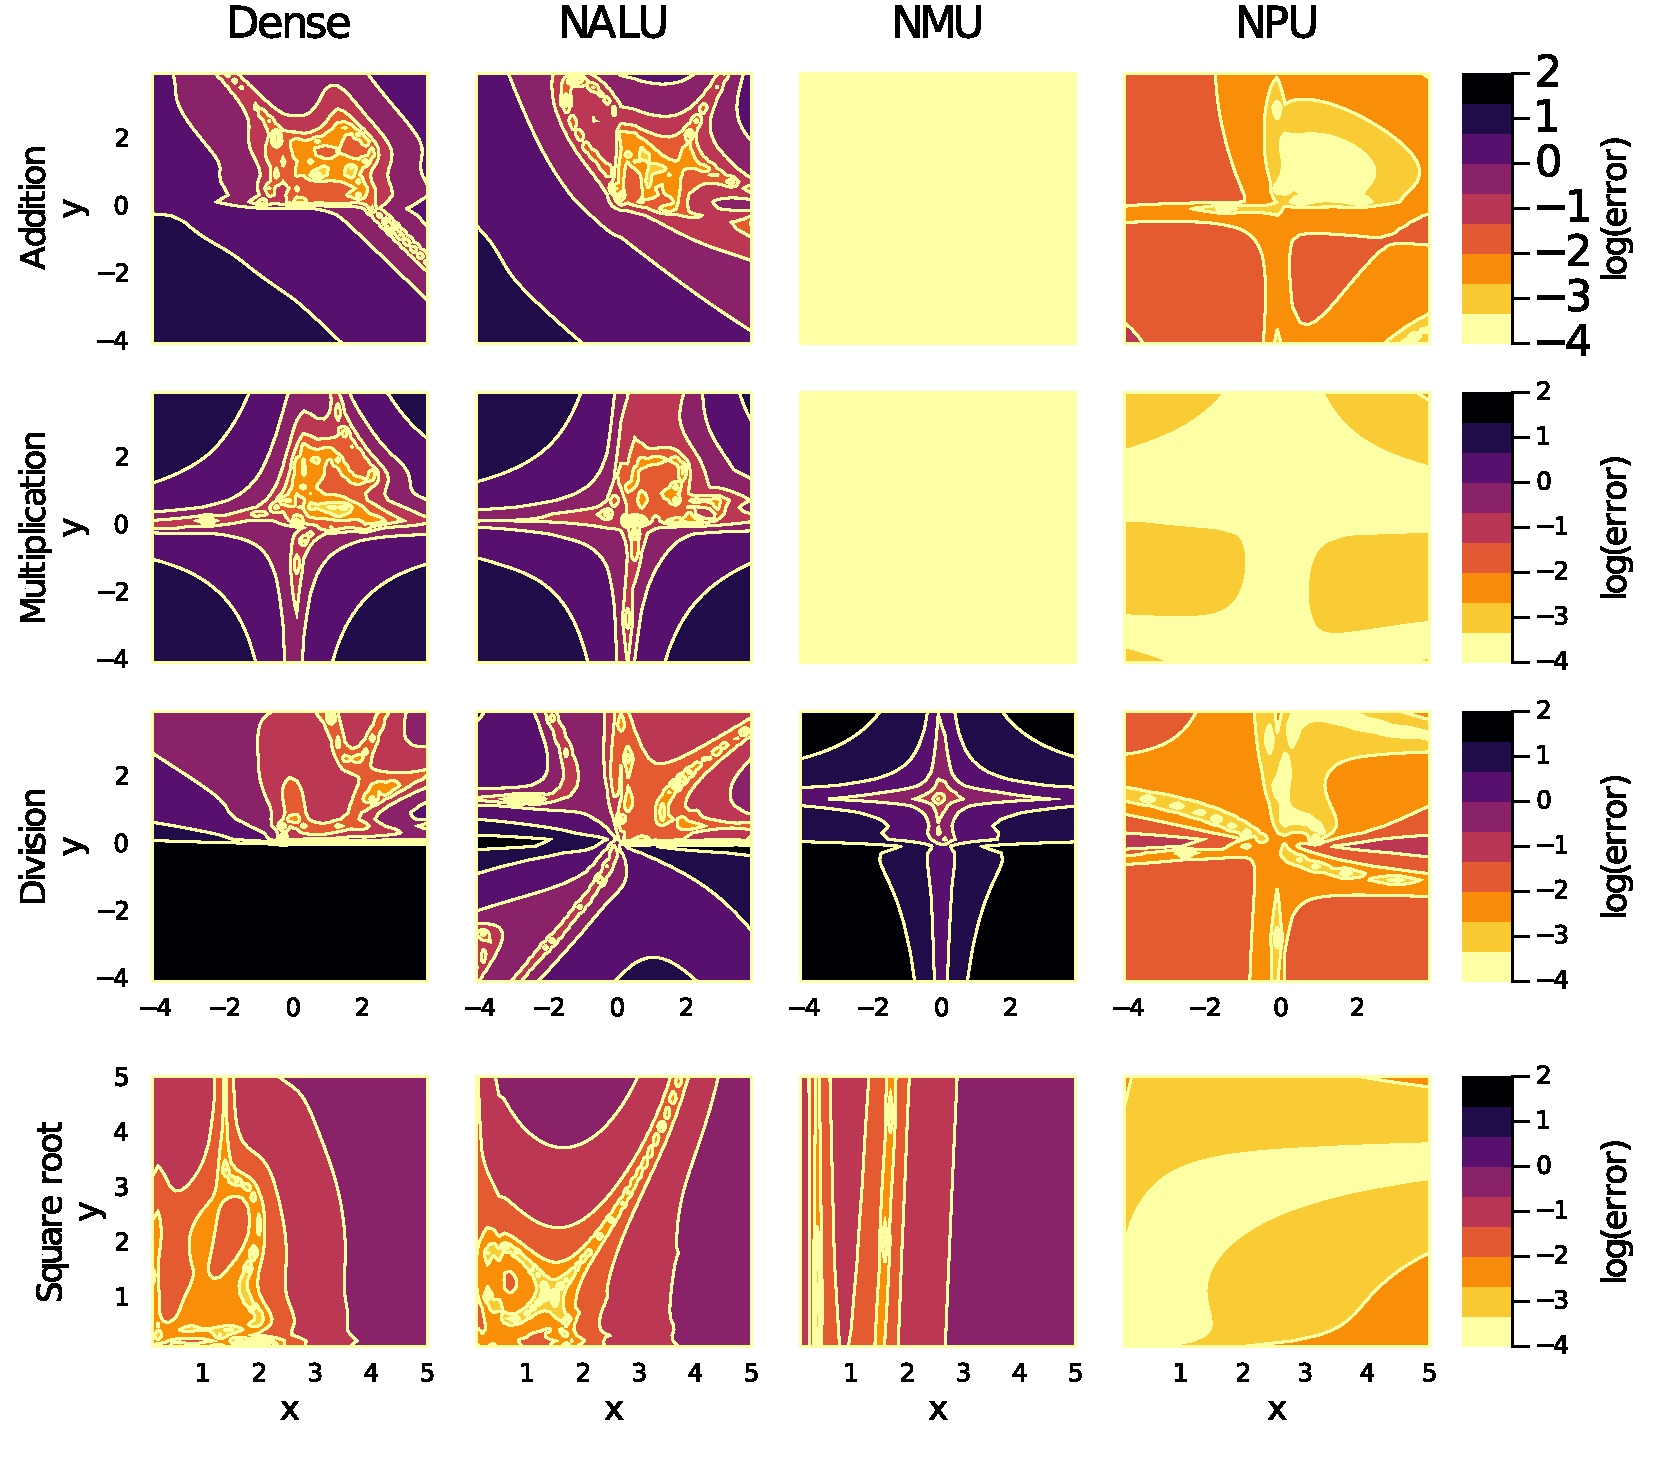
\includegraphics[width=\linewidth]{../plots/small_simple_err.pdf}};
      \draw[white, fill=white] (2.5,0) rectangle (7.9,7.6) {};
    \end{tikzpicture}
  \end{columns}
\end{frame}


\begin{frame}
  \begin{columns}
    \column{.35\textwidth}\centering
    Task: Learn $f$ in \emph{one} model
    \begin{equation*}
      f(x,y) = (x+y, xy, \frac{x}{y}, \sqrt{y})^\intercal
    \end{equation*}

    \column{.65\textwidth}
    \begin{tikzpicture}
      \node[anchor=south west, inner sep=0] at (0,0) {
        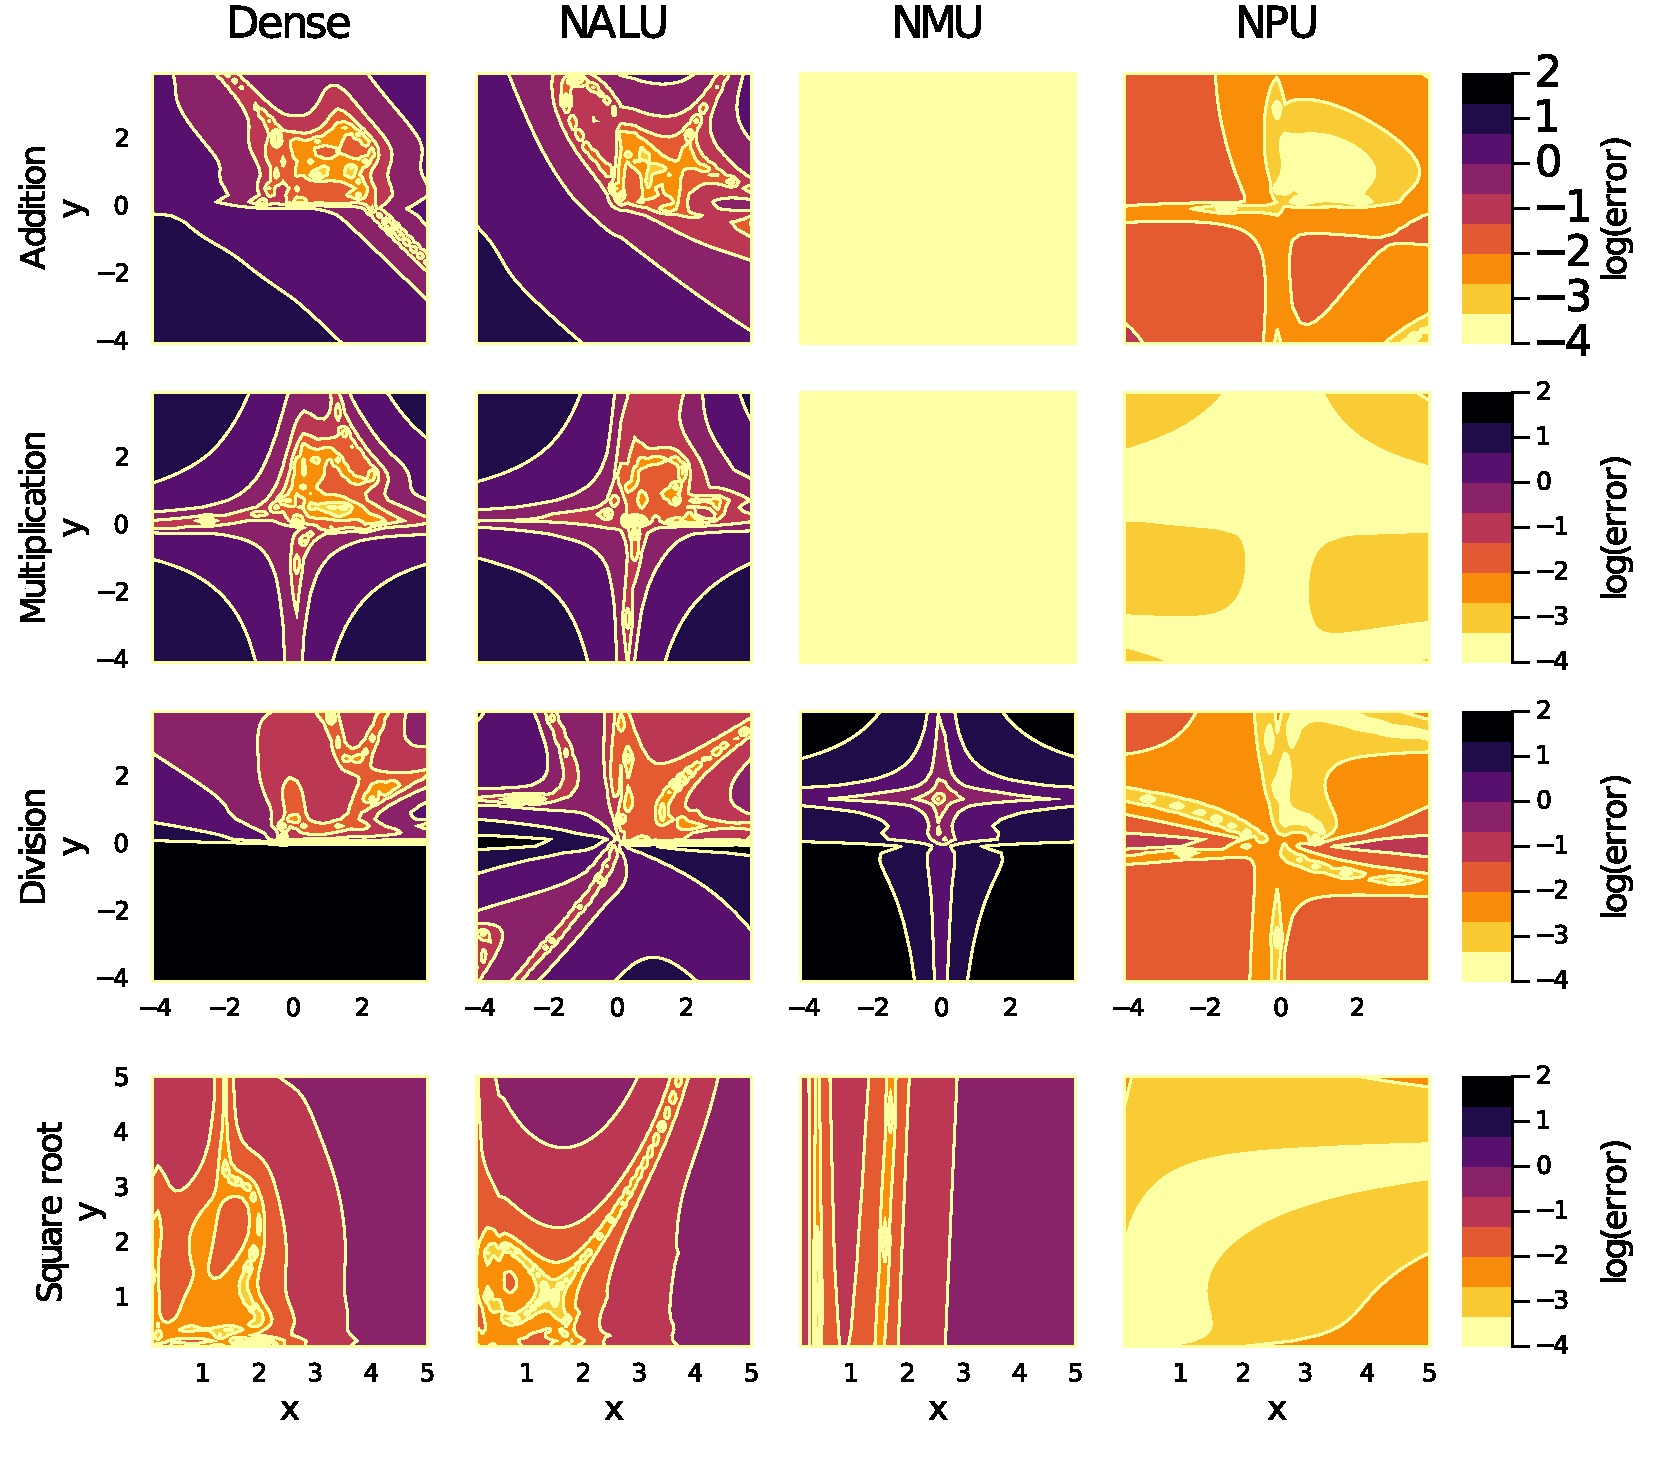
\includegraphics[width=\linewidth]{../plots/small_simple_err.pdf}};
      \draw[white, fill=white] (4.2,0) rectangle (7.9,7.6) {};
    \end{tikzpicture}
  \end{columns}
\end{frame}

\begin{frame}{Simpler Arithmetic Units}
  \begin{columns}
    \column{.5\textwidth}\centering
    % \documentclass[tikz,14pt,border=10pt]{standalone}
% 
% \usepackage{verbatim}
% \usepackage{bm}
% 
% \usetikzlibrary{%
%   arrows,%
%   shapes.misc,% wg. rounded rectangle
%   shapes.arrows,%
%   chains,%
%   matrix,%
%   positioning,% wg. " of "
%   scopes,%
%   decorations.pathmorphing,% /pgf/decoration/random steps | erste Graphik
%   shadows%
% }
% \begin{document}

\definecolor{c1}{HTML}{8097e9}
\definecolor{c2}{HTML}{c6dea2}
\definecolor{c3}{HTML}{ffb200}
\definecolor{c4}{HTML}{b6b6b6}

\tikzset{
  function/.style={
    % The shape:
    rectangle,
    rounded corners=3,
    % The size:
    minimum height=6mm,
    % The border:
    thick,
    draw=black,
    % The filling:
    top color=c1,
    bottom color=c1,
    % Font
    font=\tt
  },
  vector/.style={
    % The shape:
    rounded rectangle,
    minimum size=6mm,
    % The rest
    thick,draw=black,
    top color=c2!80,
    bottom color=c2!80,
    font=\ttfamily
  },
  trainable/.style={
    % The shape:
    diamond,
    rounded corners=3,
    minimum size=6mm,
    % The rest
    thick,draw=black,
    top color=c3!80,
    bottom color=c3!80,
    font=\ttfamily
  },
  skip loop/.style={to path={-- ++(0,#1) -| (\tikztotarget)}}
}

{
  \tikzset{vector/.append style={text height=1.5ex,text depth=.25ex}}
  \tikzset{function/.append style={text height=1.5ex,text depth=.25ex}}
}

\begin{tikzpicture}[
        point/.style={coordinate},>=stealth',thick,draw=black!90,
        tip/.style={->,shorten >=0.007pt},every join/.style={rounded corners},
        fat/.style={-, ultra thick, opacity=0.5},every join/.style={rounded corners},
        hv path/.style={to path={-| (\tikztotarget)}},
        vh path/.style={to path={|- (\tikztotarget)}},
        path/.style={to path={-- (\tikztotarget)}},
        text height=1.5ex,text depth=.25ex]

  \matrix[column sep=3mm, row sep=3mm] {
    \node (x) [vector] {$\bm x$}; &
    \node (*) [function] {$\mathrm{matmul}$}; &
    \node (y) [vector] {$\bm y$}; \\

    \node (A) [trainable] {$\bm A$}; &
    \node (clip) [function] {$\mathrm{clip}$}; \\
  };

  { [start chain];
    \chainin (x);
    \chainin (*) [join=by tip];
    \chainin (y) [join=by tip];
  }
  { [start chain];
    \chainin (A);
    \chainin (clip) [join=by tip];
    \chainin (*) [join=by tip];
  }
\end{tikzpicture}

% \end{document}


    \column{.5\textwidth}\centering
    \textbf{Neural Addition Unit (NAU)} 
    \begin{align*}
      \bm y &= \mathrm{clip}(\bm A) \cdot \bm x\\
      \mathrm{clip}(\bm M) &= \min(\max(\bm M,-1),1)
    \end{align*}
  \end{columns}
  \vfill
  \begin{columns}
    \column{.5\textwidth}\centering
    % \documentclass[tikz,14pt,border=10pt]{standalone}
% 
% \usepackage{verbatim}
% \usepackage{bm}
% 
% \usetikzlibrary{%
%   arrows,%
%   shapes.misc,% wg. rounded rectangle
%   shapes.arrows,%
%   chains,%
%   matrix,%
%   positioning,% wg. " of "
%   scopes,%
%   decorations.pathmorphing,% /pgf/decoration/random steps | erste Graphik
%   shadows%
% }
% \begin{document}

\definecolor{c1}{HTML}{8097e9}
\definecolor{c2}{HTML}{c6dea2}
\definecolor{c3}{HTML}{ffb200}
\definecolor{c4}{HTML}{b6b6b6}

\tikzset{
  function/.style={
    % The shape:
    rectangle,
    rounded corners=3,
    % The size:
    minimum height=6mm,
    % The border:
    thick,
    draw=black,
    % The filling:
    top color=c1,
    bottom color=c1,
    % Font
    font=\tt
  },
  vector/.style={
    % The shape:
    rounded rectangle,
    minimum size=6mm,
    % The rest
    thick,draw=black,
    top color=c2!80,
    bottom color=c2!80,
    font=\ttfamily
  },
  trainable/.style={
    % The shape:
    diamond,
    rounded corners=3,
    minimum size=6mm,
    % The rest
    thick,draw=black,
    top color=c3!80,
    bottom color=c3!80,
    font=\ttfamily
  },
  skip loop/.style={to path={-- ++(0,#1) -| (\tikztotarget)}}
}

{
  \tikzset{vector/.append style={text height=1.5ex,text depth=.25ex}}
  \tikzset{function/.append style={text height=1.5ex,text depth=.25ex}}
}

\begin{tikzpicture}[
        point/.style={coordinate},>=stealth',thick,draw=black!90,
        tip/.style={->,shorten >=0.007pt},every join/.style={rounded corners},
        fat/.style={-, ultra thick, opacity=0.5},every join/.style={rounded corners},
        hv path/.style={to path={-| (\tikztotarget)}},
        vh path/.style={to path={|- (\tikztotarget)}},
        path/.style={to path={-- (\tikztotarget)}},
        text height=1.5ex,text depth=.25ex]

  \matrix[column sep=3mm, row sep=3mm] {
    \node (x) [vector] {$\bm x$}; &
    \node (prod) [function] {$\mathrm{prod}$}; &
    \node (y) [vector] {$y_j$}; \\

    \node (M) [trainable] {$\bm M_{:,j}$}; &
    \node (clip) [function] {$\mathrm{clip}$}; \\
  };

  { [start chain];
    \chainin (x);
    \chainin (prod) [join=by tip];
    \chainin (y) [join=by tip];
  }
  { [start chain];
    \chainin (M);
    \chainin (clip) [join=by tip];
    \chainin (prod) [join=by tip];
  }


\end{tikzpicture}

% \end{document}


    \column{.5\textwidth}\centering
    \textbf{Neural Multiplication Unit (NMU)} 
    \begin{align*}
      \mathrm{prod}(\bm x, \hat{\bm M}_{:,j}) &= \prod_i \hat M_{ij} x_i -1 + \hat M_{ij}\\
      \mathrm{clip}(\bm M) &= \min(\max(\bm M,0),1)
    \end{align*}
  \end{columns}

  \vfill
  {\tiny(\emph{Neural Arithmetic Units}  - Madsen \& Johansen 2020)}
\end{frame}

\begin{frame}
  \begin{columns}
    \column{.35\textwidth}\centering
    Task: Learn $f$ in \emph{one} model
    \begin{equation*}
      f(x,y) = (x+y, xy, \frac{x}{y}, \sqrt{y})^\intercal
    \end{equation*}

    \column{.65\textwidth}
    \begin{tikzpicture}
      \node[anchor=south west, inner sep=0] at (0,0) {
        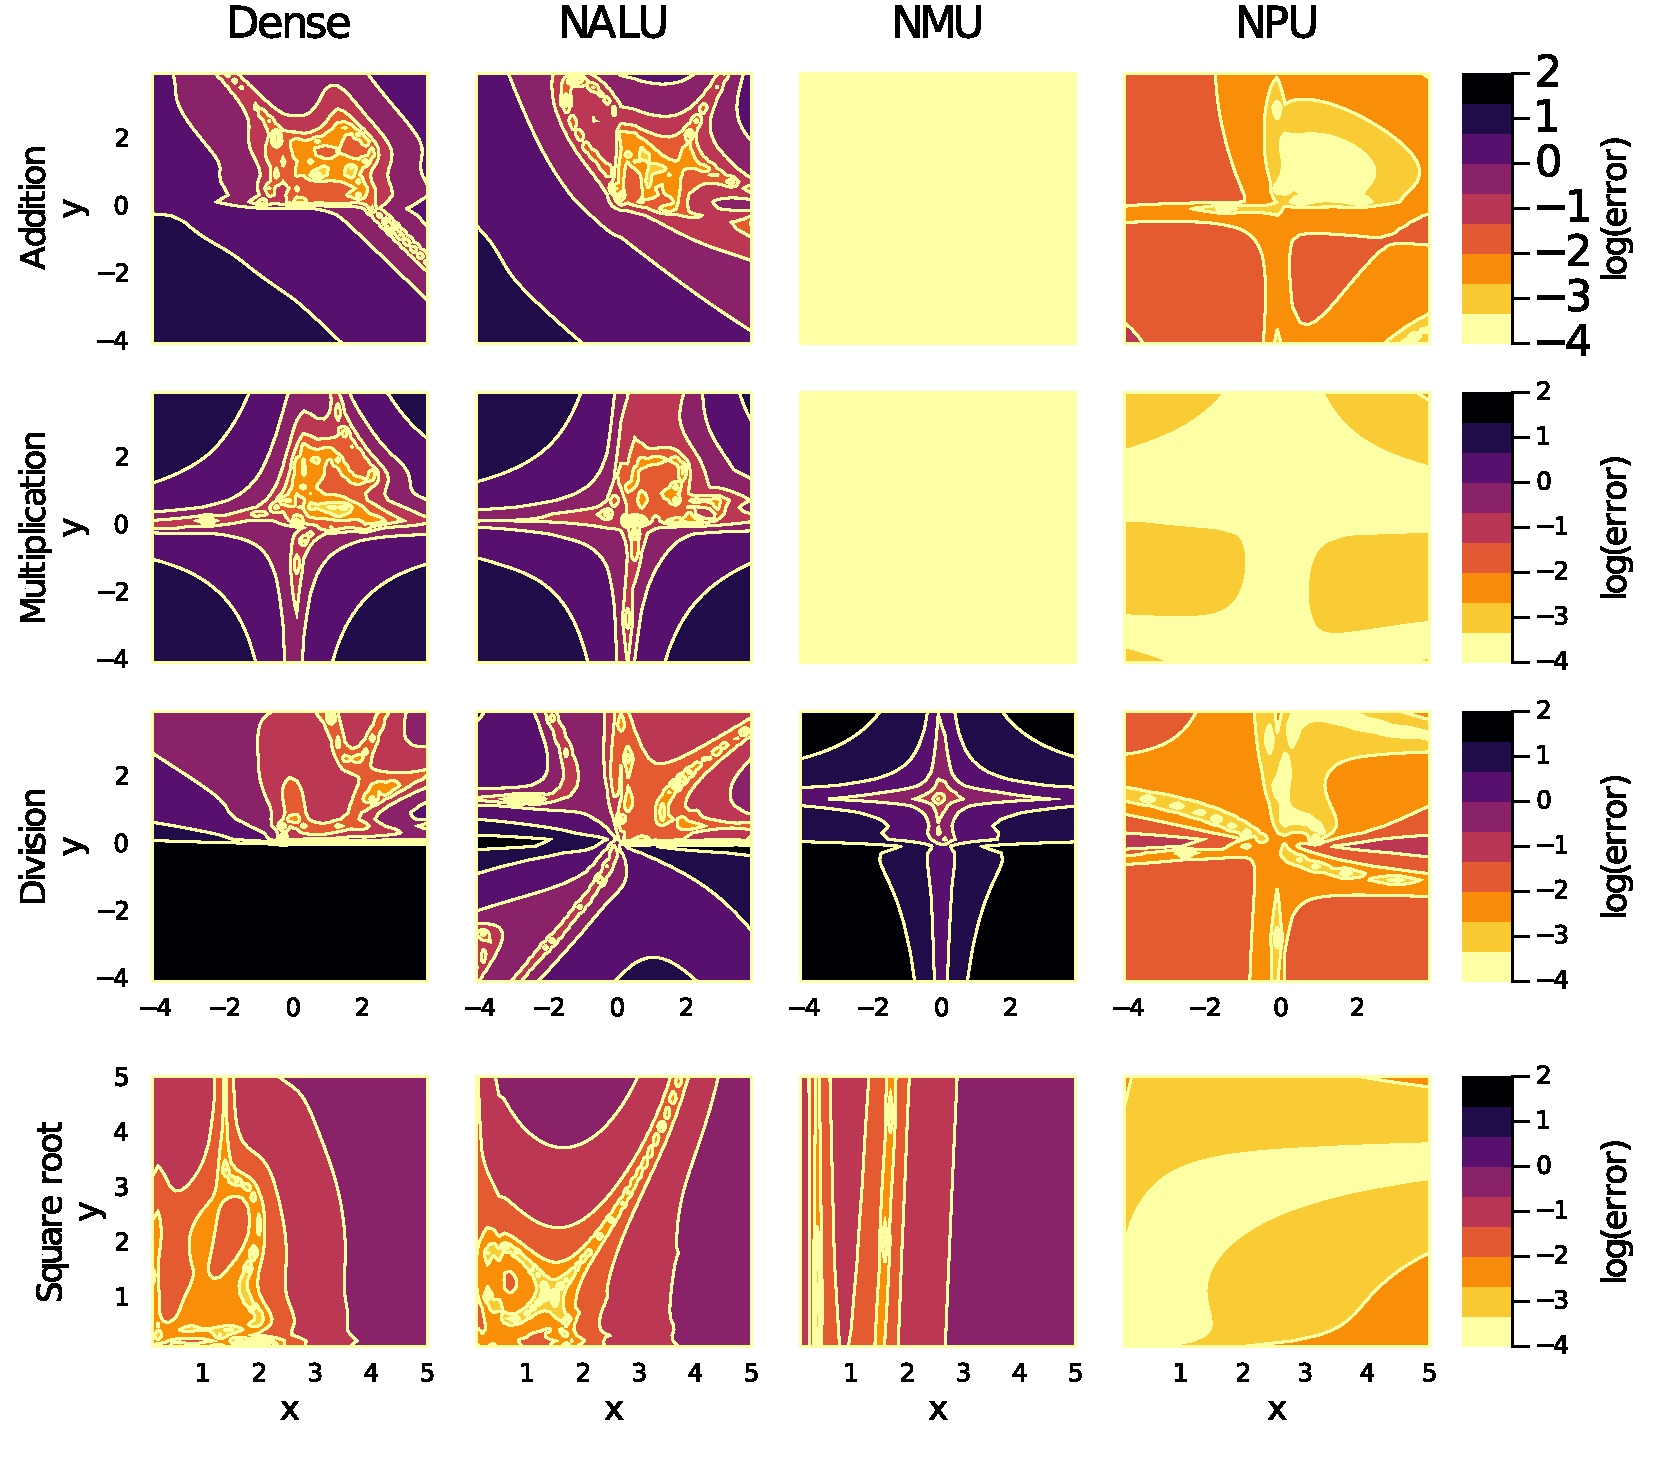
\includegraphics[width=\linewidth]{../plots/small_simple_err.pdf}};
      \draw[white, fill=white] (6.1,0) rectangle (7.9,7.6) {};
    \end{tikzpicture}
  \end{columns}
\end{frame}

\begin{frame}{Complex space}
  We extend NALU by isolating its multiplication path
  \begin{align*}
    \bm m = \exp (\bm W\log|\bm x|)
  \end{align*}
  and lifting it into complex space ($\logc$ is the complex logarithm)
  \begin{align*}
    \bm z = \real(\exp(\bm W_\mathbb{C}\logc \bm x)) = \real(\exp\left((\Wre + i\Wim) \logc\bm x\right)).
  \end{align*}
\end{frame}


\begin{frame}{Naive Neural Power Unit}
  \begin{columns}
    \column{.5\textwidth}
    % \documentclass[tikz,14pt,border=10pt]{standalone}
% 
% \usepackage{verbatim}
% \usepackage{bm}
% 
% \usetikzlibrary{%
%   arrows,%
%   shapes.misc,% wg. rounded rectangle
%   shapes.arrows,%
%   chains,%
%   matrix,%
%   positioning,% wg. " of "
%   scopes,%
%   decorations.pathmorphing,% /pgf/decoration/random steps | erste Graphik
%   shadows%
% }
% \begin{document}

\definecolor{c1}{HTML}{8097e9}
\definecolor{c2}{HTML}{c6dea2}
\definecolor{c3}{HTML}{ffb200}
\definecolor{c4}{HTML}{b6b6b6}

\tikzset{
  function/.style={
    % The shape:
    rectangle,
    rounded corners=3,
    % The size:
    minimum height=6mm,
    % The border:
    thick,
    draw=black,
    % The filling:
    top color=c1,
    bottom color=c1,
    % Font
    font=\tt
  },
  vector/.style={
    % The shape:
    rounded rectangle,
    minimum size=6mm,
    % The rest
    thick,draw=black,
    top color=c2!80,
    bottom color=c2!80,
    font=\ttfamily
  },
  trainable/.style={
    % The shape:
    diamond,
    rounded corners=3,
    minimum size=6mm,
    % The rest
    thick,draw=black,
    top color=c3!80,
    bottom color=c3!80,
    font=\ttfamily
  },
  skip loop/.style={to path={-- ++(0,#1) -| (\tikztotarget)}}
}

{
  \tikzset{vector/.append style={text height=1.5ex,text depth=.25ex}}
  \tikzset{function/.append style={text height=1.5ex,text depth=.25ex}}
}

\begin{tikzpicture}[
        point/.style={coordinate},>=stealth',thick,draw=black!90,
        tip/.style={->,shorten >=0.007pt},every join/.style={rounded corners},
        fat/.style={-, ultra thick, opacity=0.5},every join/.style={rounded corners},
        path/.style={to path={-- (\tikztotarget)}},
        hv path/.style={to path={-| (\tikztotarget)}},
        vh path/.style={to path={|- (\tikztotarget)}},
        text height=1.5ex,text depth=.25ex]

  \matrix[column sep=3mm, row sep=3mm] {
    & \node (abs) [function] {$\mathrm{abs}$}; &
    \node (r) [vector] {$\bm r$}; & &
    \node (mult) [function] {$\mathrm{mult}$}; \\

    \node (x) [vector] {$\bm x$}; & & & &
    \node (wr) [trainable] {$\bm W_r$}; & \node (wi) [trainable] {$\bm W_i$}; &
    \node (odot) [function] {$\odot$}; &
    \node (y) [vector] {$\bm y$};\\

    & \node (bin) [function] {$\mathrm{bin}$}; &
    \node (k) [vector] {$\bm k$}; & &
    \node (sign) [function] {$\mathrm{sign}$}; \\
  };

  { [start chain]
    \chainin (x);
    \chainin (abs) [join=by {tip, vh path}];
    \chainin (r) [join=by path];
    \chainin (mult) [join=by tip];
    \chainin (odot) [join=by {hv path, tip}];
    \chainin (y) [join=by tip];
  }
  { [start chain]
    \chainin (x);
    \chainin (bin) [join=by {tip, vh path}];
    \chainin (k) [join=by path];
    \chainin (sign) [join=by tip];
    \chainin (odot) [join=by {tip, hv path}];
  }
  { [start chain] \chainin (wr); \chainin (mult) [join=by tip]; }
  { [start chain] \chainin (wr); \chainin (sign) [join=by tip]; }
  { [start chain] \chainin (wi); \chainin (mult) [join=by tip]; }
  { [start chain] \chainin (wi); \chainin (sign) [join=by tip]; }
  { [start chain] \chainin (r); \chainin (sign) [join=by tip]; }
  { [start chain] \chainin (k); \chainin (mult) [join=by tip]; }

\end{tikzpicture}

% \end{document}


    \column{.5\textwidth}
    \begin{align*}
      \mult(\bm r,\bm k,\Wre,\Wim) &= \exp(\Wre \log \bm r - \pi\Wim \bm k) \\
      \sign(\bm r,\bm k,\Wre,\Wim) &= \cos(\Wim \log \bm r + \pi\Wre \bm k) \\
    \end{align*}
    \begin{align*}
      \abs(\bm x)              &= \bm r = |\bm x| + \epsilon \\
      \bin(x_i)            &= k_i = \begin{cases}
         0  & x_i \geq 0 \\
         1 & x_i < 0
      \end{cases}
    \end{align*}

  \end{columns}
\end{frame}


\begin{frame}{Neural Power Unit}
  \begin{columns}
    \column{.5\textwidth}
      % \documentclass[tikz,14pt,border=10pt]{standalone}
% 
% \usepackage{verbatim}
% \usepackage{bm}
% 
% \usetikzlibrary{%
%   arrows,%
%   shapes.misc,% wg. rounded rectangle
%   shapes.arrows,%
%   chains,%
%   matrix,%
%   positioning,% wg. " of "
%   scopes,%
%   decorations.pathmorphing,% /pgf/decoration/random steps | erste Graphik
%   shadows%
% }
% \begin{document}

\definecolor{c1}{HTML}{8097e9}
\definecolor{c2}{HTML}{c6dea2}
\definecolor{c3}{HTML}{ffb200}
\definecolor{c4}{HTML}{b6b6b6}

\tikzset{
  function/.style={
    % The shape:
    rectangle,
    rounded corners=4,
    % The size:
    minimum height=6mm,
    % The border:
    thick,
    draw=black,         % 50% red and 50% black,
                                  % and that mixed with 50% white
    % The filling:
    top color=c1,              % a shading that is white at the top...
    bottom color=c1, % and something else at the bottom
    % Font
    font=\tt
  },
  vector/.style={
    % The shape:
    rounded rectangle,
    minimum size=6mm,
    % The rest
    thick,draw=black,
    top color=c2!80,
    bottom color=c2!80,
    font=\ttfamily},
  weight/.style={
    % The shape:
    rounded rectangle,
    minimum size=6mm,
    % The rest
    thick,draw=black,
    top color=c3!80,
    bottom color=c3!80,
    font=\ttfamily},
  skip loop/.style={to path={-- ++(0,#1) -| (\tikztotarget)}}
}

{
  \tikzset{vector/.append style={text height=1.5ex,text depth=.25ex}}
  \tikzset{function/.append style={text height=1.5ex,text depth=.25ex}}
}

\begin{tikzpicture}[
        point/.style={coordinate},>=stealth',thick,draw=black!90,
        tip/.style={->,shorten >=0.007pt},every join/.style={rounded corners},
        fat/.style={-, ultra thick, opacity=0.5},every join/.style={rounded corners},
        hv path/.style={to path={-| (\tikztotarget)}},
        vh path/.style={to path={|- (\tikztotarget)}},
        text height=1.5ex,text depth=.25ex % align text horizontally
    ]
    \fill [c4, rounded corners=20, draw, opacity=0.5] (-7.7,-2.0) rectangle (7.6,2.0);
    \fill [c4, draw, pattern=north west lines, pattern color=c4] (-4.9,-2.0) rectangle (-0.9,2.0);
    \matrix[column sep=2mm, row sep=1mm] {
      % First row
      & & \node (r) [vector] {$\bm r$};& & \node (m1) [function] {$\bm\odot$}; & &
        \node (a1) [function] {$\bm +$}; & &
        \node (log) [function] {log}; & &
        \node (wr1) [function] {matmul}; & & \\

      % Second row
      & \node (abs) [function] {abs}; & & & & & & & & & &
        \node (wi1) [function] {matmul};& & \node (plus) [function] {$\bm -$}; & &
        \node (exp) [function] {exp};\\

      % middle row
      \node (in) [vector] {$\bm x$}; & \node (p2) [point] {};& & \node (g) [weight] {$\bm g$}; &
      \node (clip) [function] {clip 0 1}; & & \node (minusone) [function] {1-g}; & & & &
      \node (wr) [weight] {$\bm W_r$}; & \node (wi) [weight] {$\bm W_i$}; & & & & &
      \node (mul) [function] {$\bm\odot$}; & &
      \node (out) [vector] {$\bm y$};\\

      % fourth row
      & \node (0pi) [function] {0:$\pi$}; & & & & & & & & & &
        \node (wi2) [function] {matmul};& & \node (minus) [function] {$\bm +$};& &
        \node (cos) [function] {cos};\\

      % bottom row
      & & \node (k) [vector] {$\bm k$}; & & \node (m2) [function] {$\bm\odot$}; & & & & &
          \node (beforewr2) [point] {}; & 
        \node (wr2) [function] {matmul}; & & & \\
    };

    { [start chain]
      \chainin (in);
      \chainin (p2) [join];
      { [start branch=rbr]
        \chainin (abs) [join];
        \chainin (r) [join=by {vh path}];
        \chainin (m1) [join=by tip];
        \chainin (a1) [join=by tip];
        \chainin (log) [join=by tip];
        { [start branch=rbrup]
          \chainin (wr1) [join=by tip];
          \chainin (plus) [join=by {tip, hv path}];
        }
        { [start branch=rbrdown]
          \chainin (wi2) [join=by {vh path, tip}];
          \chainin (minus) [join=by tip];
        }
        \chainin (plus);
        \chainin (exp) [join=by tip];
        \chainin (mul) [join=by {hv path,tip}];
      }
      { [start branch=kbr]
        \chainin (0pi) [join];
        \chainin (k) [join=by {vh path}];
        \chainin (m2) [join=by tip];
        \chainin (beforewr2) [join];
        { [start branch=kbrdown]
          \chainin (wr2) [join=by tip];
          \chainin (minus) [join=by {hv path,tip}];
        }
        { [start branch=kbrup]
          \chainin (wi1) [join=by {vh path,tip}];
          \chainin (plus) [join=by tip];
        }
        \chainin (minus);
        \chainin (cos) [join=by tip];
        \chainin (mul) [join=by {hv path,tip}];
        \chainin (out) [join=by tip];
      }
    }

    { [start chain]
      \chainin (g);
      \chainin (clip) [join=by fat];
      \chainin (m1) [join=by tip];
    }

    { [start chain]
      \chainin (clip);
      \chainin (m2) [join=by tip];
    }

    { [start chain]
      \chainin (clip);
      \chainin (minusone) [join=by tip];
      \chainin (a1) [join=by tip];
    }

    { [start chain]
      \chainin (wr2);
      \chainin (wr) [join=by fat];
      \chainin (wr1) [join=by fat];
    }

    { [start chain]
      \chainin (wi2);
      \chainin (wi) [join=by fat];
      \chainin (wi1) [join=by fat];
    }


\end{tikzpicture}

% \end{document}


    \column{.5\textwidth}
      \begin{align*}
        \mult(\bm r,\bm k,\Wre,\Wim) &= \exp(\Wre \log \bm r - \pi\Wim \bm k) \\
        \sign(\bm r,\bm k,\Wre,\Wim) &= \cos(\Wim \log \bm r + \pi\Wre \bm k) \\
        \gate(\bm x,\bm g)           &= (\bm r,\bm k) \\
      \end{align*}
      \begin{center} where \end{center}
      \begin{align*}
        \bm r &= \hat{\bm g} \odot (|\bm x|+\epsilon) + (1-\hat{\bm g}), \\
        k_i &= \begin{cases}
           0  & x_i \geq 0 \\
          \hat g_i & x_i < 0
        \end{cases},\\
        \hat{\bm g} &= \min(\max(\bm g,0),1),
      \end{align*}
  \end{columns}
\end{frame}

\begin{frame}
  \begin{columns}
    \column{.35\textwidth}\centering
    Task: Learn $f$ in \emph{one} model
    \begin{equation*}
      f(x,y) = (x+y, xy, \frac{x}{y}, \sqrt{y})^\intercal
    \end{equation*}

    \column{.65\textwidth}
    \begin{tikzpicture}
      \node[anchor=south west, inner sep=0] at (0,0) {
        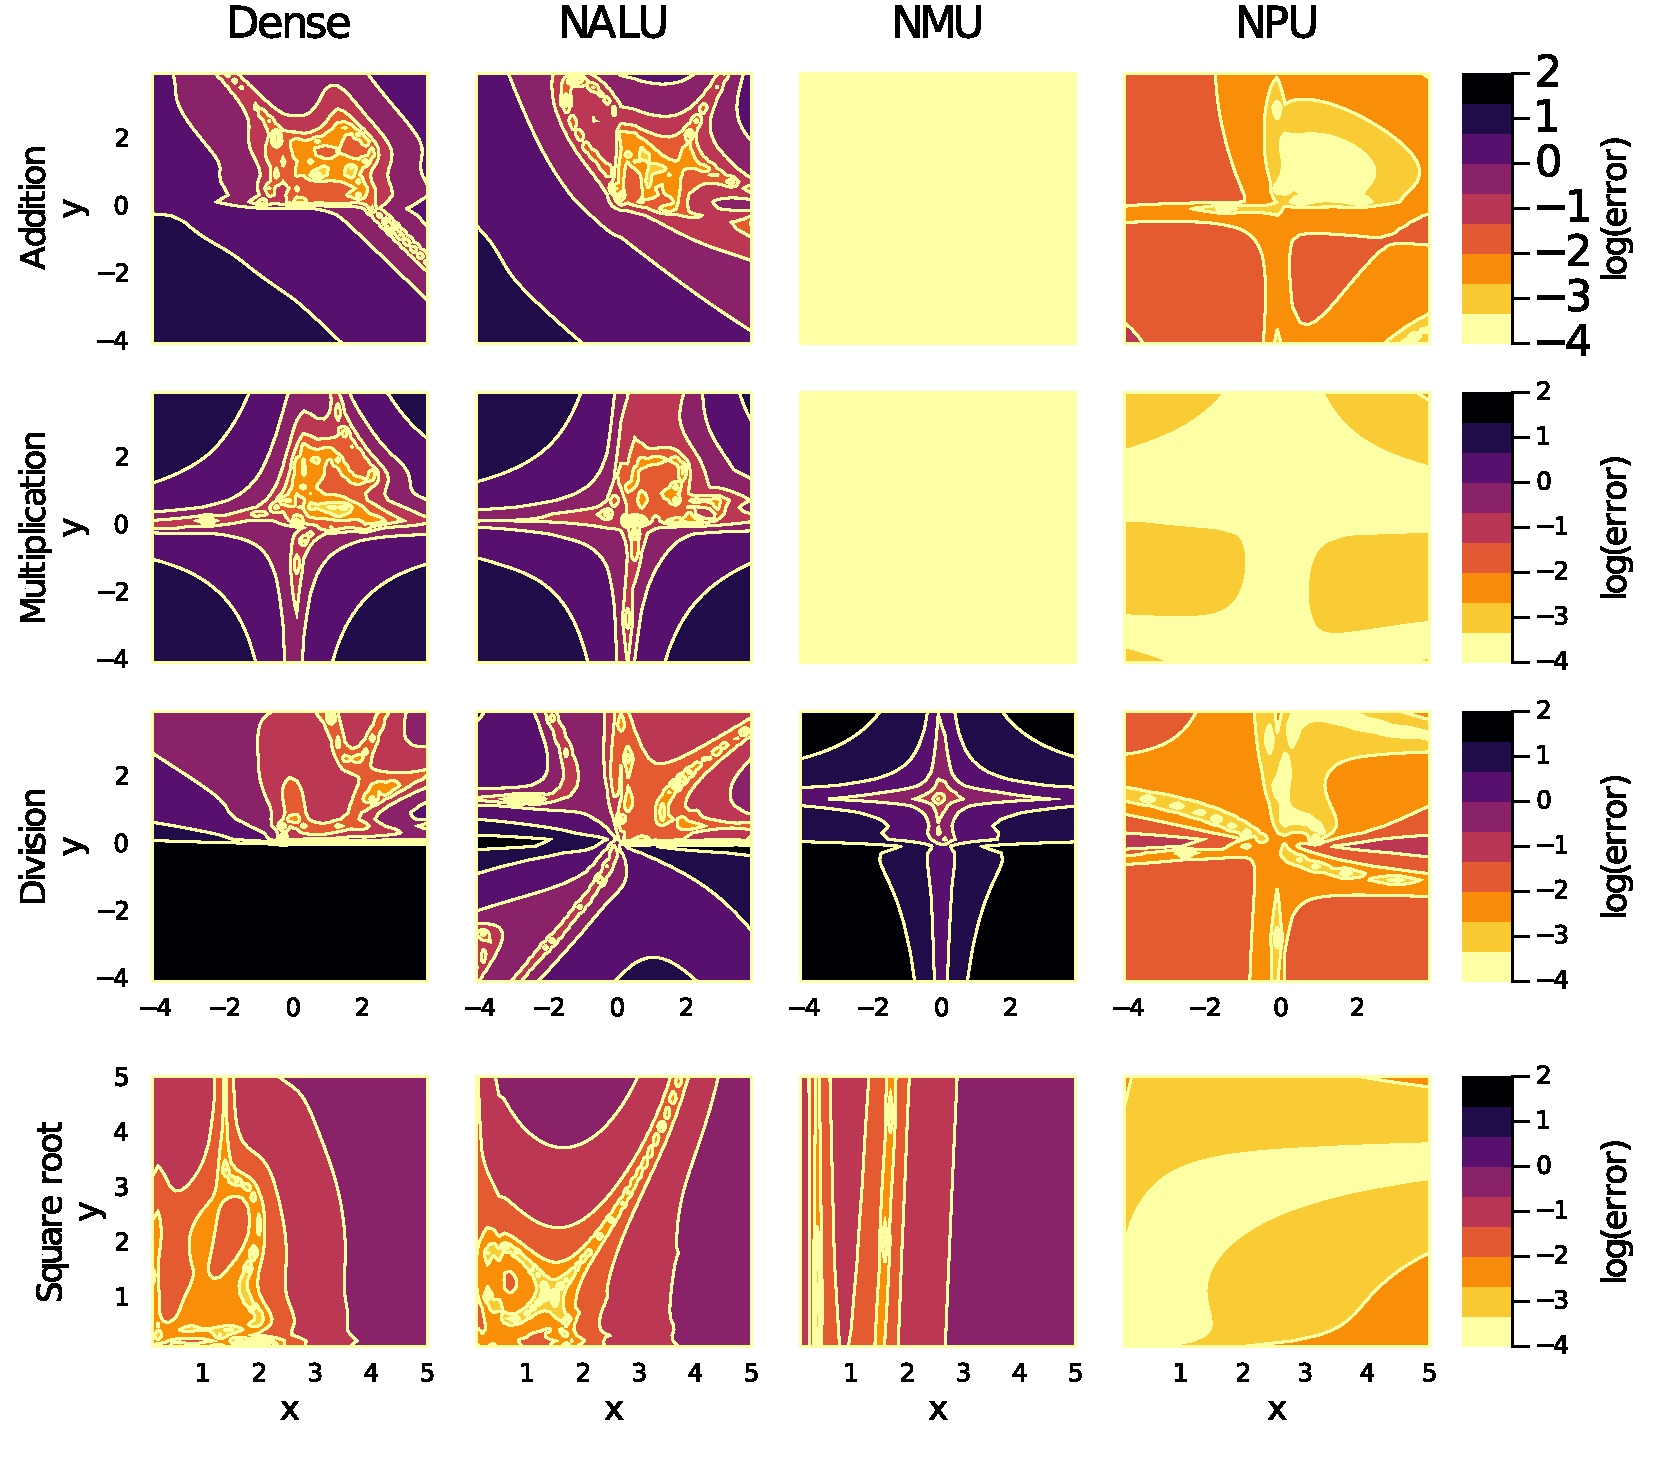
\includegraphics[width=\linewidth]{../plots/small_simple_err.pdf}};
    \end{tikzpicture}
  \end{columns}
\end{frame}

\begin{frame}{Fractional SIR}
  \begin{columns}
    \column{.5\textwidth}\centering
    \resizebox{\textwidth}{!}{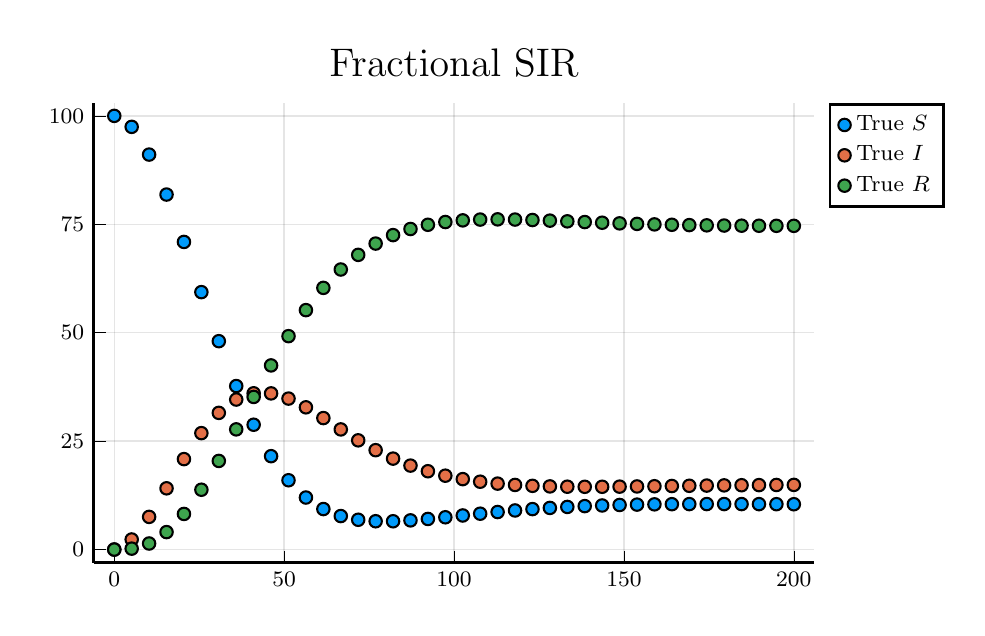
\begin{tikzpicture}[/tikz/background rectangle/.style={fill={rgb,1:red,1.0;green,1.0;blue,1.0}, draw opacity={1.0}}, show background rectangle]
\begin{axis}[point meta max={nan}, point meta min={nan}, legend cell align={left}, title={Fractional SIR}, title style={at={{(0.5,1)}}, anchor={south}, font={{\fontsize{14 pt}{18.2 pt}\selectfont}}, color={rgb,1:red,0.0;green,0.0;blue,0.0}, draw opacity={1.0}, rotate={0.0}}, legend style={color={rgb,1:red,0.0;green,0.0;blue,0.0}, draw opacity={1.0}, line width={1}, solid, fill={rgb,1:red,1.0;green,1.0;blue,1.0}, fill opacity={1.0}, text opacity={1.0}, font={{\fontsize{8 pt}{10.4 pt}\selectfont}}, at={(1.02, 1)}, anchor={north west}}, axis background/.style={fill={rgb,1:red,1.0;green,1.0;blue,1.0}, opacity={1.0}}, anchor={north west}, xshift={1.0mm}, yshift={-1.0mm}, width={107.3mm}, height={74.2mm}, scaled x ticks={false}, xlabel={}, x tick style={color={rgb,1:red,0.0;green,0.0;blue,0.0}, opacity={1.0}}, x tick label style={color={rgb,1:red,0.0;green,0.0;blue,0.0}, opacity={1.0}, rotate={0}}, xlabel style={at={(ticklabel cs:0.5)}, anchor=near ticklabel, font={{\fontsize{11 pt}{14.3 pt}\selectfont}}, color={rgb,1:red,0.0;green,0.0;blue,0.0}, draw opacity={1.0}, rotate={0.0}}, xmajorgrids={true}, xmin={-6.0}, xmax={206.0}, xtick={{0.0,50.0,100.0,150.0,200.0}}, xticklabels={{$0$,$50$,$100$,$150$,$200$}}, xtick align={inside}, xticklabel style={font={{\fontsize{8 pt}{10.4 pt}\selectfont}}, color={rgb,1:red,0.0;green,0.0;blue,0.0}, draw opacity={1.0}, rotate={0.0}}, x grid style={color={rgb,1:red,0.0;green,0.0;blue,0.0}, draw opacity={0.1}, line width={0.5}, solid}, axis x line*={left}, x axis line style={color={rgb,1:red,0.0;green,0.0;blue,0.0}, draw opacity={1.0}, line width={1}, solid}, scaled y ticks={false}, ylabel={}, y tick style={color={rgb,1:red,0.0;green,0.0;blue,0.0}, opacity={1.0}}, y tick label style={color={rgb,1:red,0.0;green,0.0;blue,0.0}, opacity={1.0}, rotate={0}}, ylabel style={at={(ticklabel cs:0.5)}, anchor=near ticklabel, font={{\fontsize{11 pt}{14.3 pt}\selectfont}}, color={rgb,1:red,0.0;green,0.0;blue,0.0}, draw opacity={1.0}, rotate={0.0}}, ymajorgrids={true}, ymin={-3.0}, ymax={103.0}, ytick={{0.0,25.0,50.0,75.0,100.0}}, yticklabels={{$0$,$25$,$50$,$75$,$100$}}, ytick align={inside}, yticklabel style={font={{\fontsize{8 pt}{10.4 pt}\selectfont}}, color={rgb,1:red,0.0;green,0.0;blue,0.0}, draw opacity={1.0}, rotate={0.0}}, y grid style={color={rgb,1:red,0.0;green,0.0;blue,0.0}, draw opacity={0.1}, line width={0.5}, solid}, axis y line*={left}, y axis line style={color={rgb,1:red,0.0;green,0.0;blue,0.0}, draw opacity={1.0}, line width={1}, solid}]
    \addplot[color={rgb,1:red,0.0;green,0.6056;blue,0.9787}, name path={ff64db2e-901e-4e78-9819-336f9c96564f}, only marks, draw opacity={1.0}, line width={0}, solid, mark={*}, mark size={2.25 pt}, mark repeat={1}, mark options={color={rgb,1:red,0.0;green,0.0;blue,0.0}, draw opacity={1.0}, fill={rgb,1:red,0.0;green,0.6056;blue,0.9787}, fill opacity={1.0}, line width={0.75}, rotate={0}, solid}]
        table[row sep={\\}]
        {
            \\
            0.0  100.0  \\
            5.128205128205129  97.46721309713212  \\
            10.256410256410257  91.07411529978752  \\
            15.384615384615385  81.85822003827998  \\
            20.512820512820515  70.93406989207153  \\
            25.641025641025642  59.36171599653322  \\
            30.76923076923077  48.05121932732702  \\
            35.8974358974359  37.70386572153941  \\
            41.02564102564103  28.786661655619767  \\
            46.15384615384615  21.536458098202502  \\
            51.282051282051285  15.984367444258964  \\
            56.41025641025641  12.000464352759552  \\
            61.53846153846154  9.344211354396093  \\
            66.66666666666667  7.730064928992786  \\
            71.7948717948718  6.871778028659456  \\
            76.92307692307692  6.531712440790295  \\
            82.05128205128206  6.527846168986343  \\
            87.17948717948718  6.732261015727868  \\
            92.3076923076923  7.058906461697017  \\
            97.43589743589743  7.448852247665159  \\
            102.56410256410257  7.8621381580828835  \\
            107.6923076923077  8.271957039163652  \\
            112.82051282051282  8.660383314615434  \\
            117.94871794871794  9.015599814052901  \\
            123.07692307692308  9.330728378580337  \\
            128.2051282051282  9.603063253817359  \\
            133.33333333333334  9.832194944069075  \\
            138.46153846153845  10.019480104740795  \\
            143.5897435897436  10.168236969594094  \\
            148.71794871794873  10.282830242207533  \\
            153.84615384615384  10.367552891075434  \\
            158.97435897435898  10.42665962038892  \\
            164.10256410256412  10.464984481530161  \\
            169.23076923076923  10.487122611260277  \\
            174.35897435897436  10.496809113024415  \\
            179.48717948717947  10.49696822418185  \\
            184.6153846153846  10.490486949159731  \\
            189.74358974358975  10.479876278697317  \\
            194.87179487179486  10.467010848152167  \\
            200.0  10.453187053405765  \\
        }
        ;
    \addlegendentry {True $S$}
    \addplot[color={rgb,1:red,0.8889;green,0.4356;blue,0.2781}, name path={c3f5ee68-cf52-4be0-a8ba-f0c91306ea66}, only marks, draw opacity={1.0}, line width={0}, solid, mark={*}, mark size={2.25 pt}, mark repeat={1}, mark options={color={rgb,1:red,0.0;green,0.0;blue,0.0}, draw opacity={1.0}, fill={rgb,1:red,0.8889;green,0.4356;blue,0.2781}, fill opacity={1.0}, line width={0.75}, rotate={0}, solid}]
        table[row sep={\\}]
        {
            \\
            0.0  0.01  \\
            5.128205128205129  2.326002254590468  \\
            10.256410256410257  7.535412858135904  \\
            15.384615384615385  14.122344350839555  \\
            20.512820512820515  20.861212946319004  \\
            25.641025641025642  26.852061199698944  \\
            30.76923076923077  31.52079010396936  \\
            35.8974358974359  34.589940517583635  \\
            41.02564102564103  36.03247808932137  \\
            46.15384615384615  36.0106783095002  \\
            51.282051282051285  34.81461042142043  \\
            56.41025641025641  32.799670718853136  \\
            61.53846153846154  30.321886606977262  \\
            66.66666666666667  27.70444740533231  \\
            71.7948717948718  25.186917212993873  \\
            76.92307692307692  22.920167986169474  \\
            82.05128205128206  20.97478194912876  \\
            87.17948717948718  19.361879697078066  \\
            92.3076923076923  18.06136663645284  \\
            97.43589743589743  17.0351828644295  \\
            102.56410256410257  16.243460467487697  \\
            107.6923076923077  15.64716970581006  \\
            112.82051282051282  15.209576700999039  \\
            117.94871794871794  14.900102701702954  \\
            123.07692307692308  14.692768418941395  \\
            128.2051282051282  14.564262720391902  \\
            133.33333333333334  14.495696710475123  \\
            138.46153846153845  14.472242253795276  \\
            143.5897435897436  14.480798749993546  \\
            148.71794871794873  14.510674957112856  \\
            153.84615384615384  14.553801666023665  \\
            158.97435897435898  14.60424306180992  \\
            164.10256410256412  14.656998699052162  \\
            169.23076923076923  14.708526692892267  \\
            174.35897435897436  14.75644891382746  \\
            179.48717948717947  14.799483648325703  \\
            184.6153846153846  14.836795847017735  \\
            189.74358974358975  14.868211842226707  \\
            194.87179487179486  14.893874068806547  \\
            200.0  14.91412562301017  \\
        }
        ;
    \addlegendentry {True $I$}
    \addplot[color={rgb,1:red,0.2422;green,0.6433;blue,0.3044}, name path={2548fa7f-f680-455c-9e2e-d04be11eb1cb}, only marks, draw opacity={1.0}, line width={0}, solid, mark={*}, mark size={2.25 pt}, mark repeat={1}, mark options={color={rgb,1:red,0.0;green,0.0;blue,0.0}, draw opacity={1.0}, fill={rgb,1:red,0.2422;green,0.6433;blue,0.3044}, fill opacity={1.0}, line width={0.75}, rotate={0}, solid}]
        table[row sep={\\}]
        {
            \\
            0.0  0.0  \\
            5.128205128205129  0.21678464827744337  \\
            10.256410256410257  1.4004718420766002  \\
            15.384615384615385  4.029435610880507  \\
            20.512820512820515  8.214717161609485  \\
            25.641025641025642  13.796222803767884  \\
            30.76923076923077  20.43799056870365  \\
            35.8974358974359  27.71619376087699  \\
            41.02564102564103  35.19086025505889  \\
            46.15384615384615  42.462863592297325  \\
            51.282051282051285  49.21102213432063  \\
            56.41025641025641  55.20986492838734  \\
            61.53846153846154  60.34390203862667  \\
            66.66666666666667  64.57548766567494  \\
            71.7948717948718  67.95130475834671  \\
            76.92307692307692  70.55811957304027  \\
            82.05128205128206  72.50737188188494  \\
            87.17948717948718  73.9158592871941  \\
            92.3076923076923  74.88972690185018  \\
            97.43589743589743  75.52596488790537  \\
            102.56410256410257  75.90440137442945  \\
            107.6923076923077  76.09087325502632  \\
            112.82051282051282  76.14003998438557  \\
            117.94871794871794  76.09429748424418  \\
            123.07692307692308  75.9865032024783  \\
            128.2051282051282  75.84267402579079  \\
            133.33333333333334  75.68210834545584  \\
            138.46153846153845  75.51827764146397  \\
            143.5897435897436  75.36096428041239  \\
            148.71794871794873  75.21649480067964  \\
            153.84615384615384  75.08864544290094  \\
            158.97435897435898  74.97909731780119  \\
            164.10256410256412  74.8880168194177  \\
            169.23076923076923  74.81435069584748  \\
            174.35897435897436  74.75674197314815  \\
            179.48717948717947  74.71354812749247  \\
            184.6153846153846  74.68271720382256  \\
            189.74358974358975  74.661911879076  \\
            194.87179487179486  74.64911508304131  \\
            200.0  74.6426873235841  \\
        }
        ;
    \addlegendentry {True $R$}
\end{axis}
\end{tikzpicture}
}

    \column{.5\textwidth}\centering
    Differential Equation:
    \begin{equation*}
      \begin{bmatrix}
        \dot S \\ \dot I \\ \dot R
      \end{bmatrix}
      =
      \begin{bmatrix}
        -\beta & 0 & \eta \\
        \beta & -\alpha & 0 \\
        0 & \alpha & -\eta
      \end{bmatrix}
      \begin{bmatrix}
        I^\gamma S^\kappa \\ I \\ R
      \end{bmatrix}
    \end{equation*}
  \end{columns}
\end{frame}

\begin{frame}{Black Box Models}
  \begin{columns}
    \column{.5\textwidth}\centering
    \resizebox{\textwidth}{!}{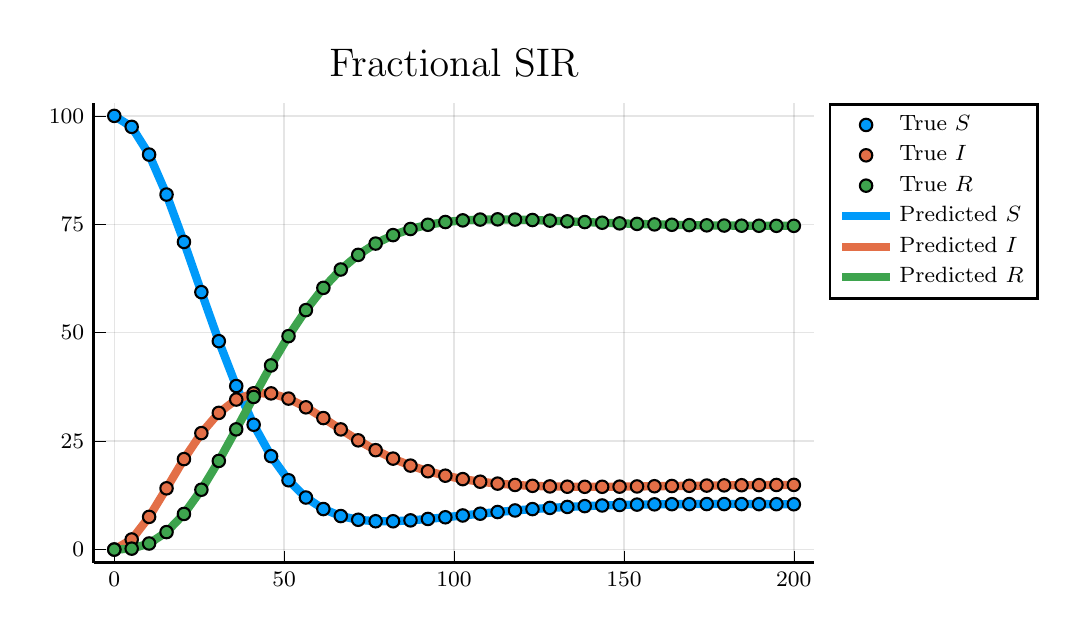
\begin{tikzpicture}[/tikz/background rectangle/.style={fill={rgb,1:red,1.0;green,1.0;blue,1.0}, draw opacity={1.0}}, show background rectangle]
\begin{axis}[point meta max={nan}, point meta min={nan}, legend cell align={left}, title={Fractional SIR}, title style={at={{(0.5,1)}}, anchor={south}, font={{\fontsize{14 pt}{18.2 pt}\selectfont}}, color={rgb,1:red,0.0;green,0.0;blue,0.0}, draw opacity={1.0}, rotate={0.0}}, legend style={color={rgb,1:red,0.0;green,0.0;blue,0.0}, draw opacity={1.0}, line width={1}, solid, fill={rgb,1:red,1.0;green,1.0;blue,1.0}, fill opacity={1.0}, text opacity={1.0}, font={{\fontsize{8 pt}{10.4 pt}\selectfont}}, at={(1.02, 1)}, anchor={north west}}, axis background/.style={fill={rgb,1:red,1.0;green,1.0;blue,1.0}, opacity={1.0}}, anchor={north west}, xshift={1.0mm}, yshift={-1.0mm}, width={107.3mm}, height={74.2mm}, scaled x ticks={false}, xlabel={}, x tick style={color={rgb,1:red,0.0;green,0.0;blue,0.0}, opacity={1.0}}, x tick label style={color={rgb,1:red,0.0;green,0.0;blue,0.0}, opacity={1.0}, rotate={0}}, xlabel style={at={(ticklabel cs:0.5)}, anchor=near ticklabel, font={{\fontsize{11 pt}{14.3 pt}\selectfont}}, color={rgb,1:red,0.0;green,0.0;blue,0.0}, draw opacity={1.0}, rotate={0.0}}, xmajorgrids={true}, xmin={-6.0}, xmax={206.0}, xtick={{0.0,50.0,100.0,150.0,200.0}}, xticklabels={{$0$,$50$,$100$,$150$,$200$}}, xtick align={inside}, xticklabel style={font={{\fontsize{8 pt}{10.4 pt}\selectfont}}, color={rgb,1:red,0.0;green,0.0;blue,0.0}, draw opacity={1.0}, rotate={0.0}}, x grid style={color={rgb,1:red,0.0;green,0.0;blue,0.0}, draw opacity={0.1}, line width={0.5}, solid}, axis x line*={left}, x axis line style={color={rgb,1:red,0.0;green,0.0;blue,0.0}, draw opacity={1.0}, line width={1}, solid}, scaled y ticks={false}, ylabel={}, y tick style={color={rgb,1:red,0.0;green,0.0;blue,0.0}, opacity={1.0}}, y tick label style={color={rgb,1:red,0.0;green,0.0;blue,0.0}, opacity={1.0}, rotate={0}}, ylabel style={at={(ticklabel cs:0.5)}, anchor=near ticklabel, font={{\fontsize{11 pt}{14.3 pt}\selectfont}}, color={rgb,1:red,0.0;green,0.0;blue,0.0}, draw opacity={1.0}, rotate={0.0}}, ymajorgrids={true}, ymin={-3.0}, ymax={103.0}, ytick={{0.0,25.0,50.0,75.0,100.0}}, yticklabels={{$0$,$25$,$50$,$75$,$100$}}, ytick align={inside}, yticklabel style={font={{\fontsize{8 pt}{10.4 pt}\selectfont}}, color={rgb,1:red,0.0;green,0.0;blue,0.0}, draw opacity={1.0}, rotate={0.0}}, y grid style={color={rgb,1:red,0.0;green,0.0;blue,0.0}, draw opacity={0.1}, line width={0.5}, solid}, axis y line*={left}, y axis line style={color={rgb,1:red,0.0;green,0.0;blue,0.0}, draw opacity={1.0}, line width={1}, solid}]
    \addplot[color={rgb,1:red,0.0;green,0.6056;blue,0.9787}, name path={1278b201-d41f-42e0-be57-354ce4d6de27}, only marks, draw opacity={1.0}, line width={0}, solid, mark={*}, mark size={2.25 pt}, mark repeat={1}, mark options={color={rgb,1:red,0.0;green,0.0;blue,0.0}, draw opacity={1.0}, fill={rgb,1:red,0.0;green,0.6056;blue,0.9787}, fill opacity={1.0}, line width={0.75}, rotate={0}, solid}]
        table[row sep={\\}]
        {
            \\
            0.0  100.0  \\
            5.128205128205129  97.46721309713212  \\
            10.256410256410257  91.07411529978752  \\
            15.384615384615385  81.85822003827998  \\
            20.512820512820515  70.93406989207153  \\
            25.641025641025642  59.36171599653322  \\
            30.76923076923077  48.05121932732702  \\
            35.8974358974359  37.70386572153941  \\
            41.02564102564103  28.786661655619767  \\
            46.15384615384615  21.536458098202502  \\
            51.282051282051285  15.984367444258964  \\
            56.41025641025641  12.000464352759552  \\
            61.53846153846154  9.344211354396093  \\
            66.66666666666667  7.730064928992786  \\
            71.7948717948718  6.871778028659456  \\
            76.92307692307692  6.531712440790295  \\
            82.05128205128206  6.527846168986343  \\
            87.17948717948718  6.732261015727868  \\
            92.3076923076923  7.058906461697017  \\
            97.43589743589743  7.448852247665159  \\
            102.56410256410257  7.8621381580828835  \\
            107.6923076923077  8.271957039163652  \\
            112.82051282051282  8.660383314615434  \\
            117.94871794871794  9.015599814052901  \\
            123.07692307692308  9.330728378580337  \\
            128.2051282051282  9.603063253817359  \\
            133.33333333333334  9.832194944069075  \\
            138.46153846153845  10.019480104740795  \\
            143.5897435897436  10.168236969594094  \\
            148.71794871794873  10.282830242207533  \\
            153.84615384615384  10.367552891075434  \\
            158.97435897435898  10.42665962038892  \\
            164.10256410256412  10.464984481530161  \\
            169.23076923076923  10.487122611260277  \\
            174.35897435897436  10.496809113024415  \\
            179.48717948717947  10.49696822418185  \\
            184.6153846153846  10.490486949159731  \\
            189.74358974358975  10.479876278697317  \\
            194.87179487179486  10.467010848152167  \\
            200.0  10.453187053405765  \\
        }
        ;
    \addlegendentry {True $S$}
    \addplot[color={rgb,1:red,0.8889;green,0.4356;blue,0.2781}, name path={fa8a375c-49f3-40d5-a7c0-8d03089f1adc}, only marks, draw opacity={1.0}, line width={0}, solid, mark={*}, mark size={2.25 pt}, mark repeat={1}, mark options={color={rgb,1:red,0.0;green,0.0;blue,0.0}, draw opacity={1.0}, fill={rgb,1:red,0.8889;green,0.4356;blue,0.2781}, fill opacity={1.0}, line width={0.75}, rotate={0}, solid}]
        table[row sep={\\}]
        {
            \\
            0.0  0.01  \\
            5.128205128205129  2.326002254590468  \\
            10.256410256410257  7.535412858135904  \\
            15.384615384615385  14.122344350839555  \\
            20.512820512820515  20.861212946319004  \\
            25.641025641025642  26.852061199698944  \\
            30.76923076923077  31.52079010396936  \\
            35.8974358974359  34.589940517583635  \\
            41.02564102564103  36.03247808932137  \\
            46.15384615384615  36.0106783095002  \\
            51.282051282051285  34.81461042142043  \\
            56.41025641025641  32.799670718853136  \\
            61.53846153846154  30.321886606977262  \\
            66.66666666666667  27.70444740533231  \\
            71.7948717948718  25.186917212993873  \\
            76.92307692307692  22.920167986169474  \\
            82.05128205128206  20.97478194912876  \\
            87.17948717948718  19.361879697078066  \\
            92.3076923076923  18.06136663645284  \\
            97.43589743589743  17.0351828644295  \\
            102.56410256410257  16.243460467487697  \\
            107.6923076923077  15.64716970581006  \\
            112.82051282051282  15.209576700999039  \\
            117.94871794871794  14.900102701702954  \\
            123.07692307692308  14.692768418941395  \\
            128.2051282051282  14.564262720391902  \\
            133.33333333333334  14.495696710475123  \\
            138.46153846153845  14.472242253795276  \\
            143.5897435897436  14.480798749993546  \\
            148.71794871794873  14.510674957112856  \\
            153.84615384615384  14.553801666023665  \\
            158.97435897435898  14.60424306180992  \\
            164.10256410256412  14.656998699052162  \\
            169.23076923076923  14.708526692892267  \\
            174.35897435897436  14.75644891382746  \\
            179.48717948717947  14.799483648325703  \\
            184.6153846153846  14.836795847017735  \\
            189.74358974358975  14.868211842226707  \\
            194.87179487179486  14.893874068806547  \\
            200.0  14.91412562301017  \\
        }
        ;
    \addlegendentry {True $I$}
    \addplot[color={rgb,1:red,0.2422;green,0.6433;blue,0.3044}, name path={b60fba55-3130-4ccc-857c-959d0c106f7a}, only marks, draw opacity={1.0}, line width={0}, solid, mark={*}, mark size={2.25 pt}, mark repeat={1}, mark options={color={rgb,1:red,0.0;green,0.0;blue,0.0}, draw opacity={1.0}, fill={rgb,1:red,0.2422;green,0.6433;blue,0.3044}, fill opacity={1.0}, line width={0.75}, rotate={0}, solid}]
        table[row sep={\\}]
        {
            \\
            0.0  0.0  \\
            5.128205128205129  0.21678464827744337  \\
            10.256410256410257  1.4004718420766002  \\
            15.384615384615385  4.029435610880507  \\
            20.512820512820515  8.214717161609485  \\
            25.641025641025642  13.796222803767884  \\
            30.76923076923077  20.43799056870365  \\
            35.8974358974359  27.71619376087699  \\
            41.02564102564103  35.19086025505889  \\
            46.15384615384615  42.462863592297325  \\
            51.282051282051285  49.21102213432063  \\
            56.41025641025641  55.20986492838734  \\
            61.53846153846154  60.34390203862667  \\
            66.66666666666667  64.57548766567494  \\
            71.7948717948718  67.95130475834671  \\
            76.92307692307692  70.55811957304027  \\
            82.05128205128206  72.50737188188494  \\
            87.17948717948718  73.9158592871941  \\
            92.3076923076923  74.88972690185018  \\
            97.43589743589743  75.52596488790537  \\
            102.56410256410257  75.90440137442945  \\
            107.6923076923077  76.09087325502632  \\
            112.82051282051282  76.14003998438557  \\
            117.94871794871794  76.09429748424418  \\
            123.07692307692308  75.9865032024783  \\
            128.2051282051282  75.84267402579079  \\
            133.33333333333334  75.68210834545584  \\
            138.46153846153845  75.51827764146397  \\
            143.5897435897436  75.36096428041239  \\
            148.71794871794873  75.21649480067964  \\
            153.84615384615384  75.08864544290094  \\
            158.97435897435898  74.97909731780119  \\
            164.10256410256412  74.8880168194177  \\
            169.23076923076923  74.81435069584748  \\
            174.35897435897436  74.75674197314815  \\
            179.48717948717947  74.71354812749247  \\
            184.6153846153846  74.68271720382256  \\
            189.74358974358975  74.661911879076  \\
            194.87179487179486  74.64911508304131  \\
            200.0  74.6426873235841  \\
        }
        ;
    \addlegendentry {True $R$}
    \addplot[color={rgb,1:red,0.0;green,0.6056;blue,0.9787}, name path={78352538-1e6c-4b6a-b132-924978ff27a2}, draw opacity={1.0}, line width={3}, solid]
        table[row sep={\\}]
        {
            \\
            0.0  100.0  \\
            5.128205128205129  97.46721309713212  \\
            10.256410256410257  91.07411529978752  \\
            15.384615384615385  81.85822003827998  \\
            20.512820512820515  70.93406989207153  \\
            25.641025641025642  59.36171599653322  \\
            30.76923076923077  48.05121932732702  \\
            35.8974358974359  37.70386572153941  \\
            41.02564102564103  28.786661655619767  \\
            46.15384615384615  21.536458098202502  \\
            51.282051282051285  15.984367444258964  \\
            56.41025641025641  12.000464352759552  \\
            61.53846153846154  9.344211354396093  \\
            66.66666666666667  7.730064928992786  \\
            71.7948717948718  6.871778028659456  \\
            76.92307692307692  6.531712440790295  \\
            82.05128205128206  6.527846168986343  \\
            87.17948717948718  6.732261015727868  \\
            92.3076923076923  7.058906461697017  \\
            97.43589743589743  7.448852247665159  \\
            102.56410256410257  7.8621381580828835  \\
            107.6923076923077  8.271957039163652  \\
            112.82051282051282  8.660383314615434  \\
            117.94871794871794  9.015599814052901  \\
            123.07692307692308  9.330728378580337  \\
            128.2051282051282  9.603063253817359  \\
            133.33333333333334  9.832194944069075  \\
            138.46153846153845  10.019480104740795  \\
            143.5897435897436  10.168236969594094  \\
            148.71794871794873  10.282830242207533  \\
            153.84615384615384  10.367552891075434  \\
            158.97435897435898  10.42665962038892  \\
            164.10256410256412  10.464984481530161  \\
            169.23076923076923  10.487122611260277  \\
            174.35897435897436  10.496809113024415  \\
            179.48717948717947  10.49696822418185  \\
            184.6153846153846  10.490486949159731  \\
            189.74358974358975  10.479876278697317  \\
            194.87179487179486  10.467010848152167  \\
            200.0  10.453187053405765  \\
        }
        ;
    \addlegendentry {Predicted $S$}
    \addplot[color={rgb,1:red,0.8889;green,0.4356;blue,0.2781}, name path={4a3ec81d-0580-419b-bf7a-1ab47488ba2a}, draw opacity={1.0}, line width={3}, solid]
        table[row sep={\\}]
        {
            \\
            0.0  0.01  \\
            5.128205128205129  2.326002254590468  \\
            10.256410256410257  7.535412858135904  \\
            15.384615384615385  14.122344350839555  \\
            20.512820512820515  20.861212946319004  \\
            25.641025641025642  26.852061199698944  \\
            30.76923076923077  31.52079010396936  \\
            35.8974358974359  34.589940517583635  \\
            41.02564102564103  36.03247808932137  \\
            46.15384615384615  36.0106783095002  \\
            51.282051282051285  34.81461042142043  \\
            56.41025641025641  32.799670718853136  \\
            61.53846153846154  30.321886606977262  \\
            66.66666666666667  27.70444740533231  \\
            71.7948717948718  25.186917212993873  \\
            76.92307692307692  22.920167986169474  \\
            82.05128205128206  20.97478194912876  \\
            87.17948717948718  19.361879697078066  \\
            92.3076923076923  18.06136663645284  \\
            97.43589743589743  17.0351828644295  \\
            102.56410256410257  16.243460467487697  \\
            107.6923076923077  15.64716970581006  \\
            112.82051282051282  15.209576700999039  \\
            117.94871794871794  14.900102701702954  \\
            123.07692307692308  14.692768418941395  \\
            128.2051282051282  14.564262720391902  \\
            133.33333333333334  14.495696710475123  \\
            138.46153846153845  14.472242253795276  \\
            143.5897435897436  14.480798749993546  \\
            148.71794871794873  14.510674957112856  \\
            153.84615384615384  14.553801666023665  \\
            158.97435897435898  14.60424306180992  \\
            164.10256410256412  14.656998699052162  \\
            169.23076923076923  14.708526692892267  \\
            174.35897435897436  14.75644891382746  \\
            179.48717948717947  14.799483648325703  \\
            184.6153846153846  14.836795847017735  \\
            189.74358974358975  14.868211842226707  \\
            194.87179487179486  14.893874068806547  \\
            200.0  14.91412562301017  \\
        }
        ;
    \addlegendentry {Predicted $I$}
    \addplot[color={rgb,1:red,0.2422;green,0.6433;blue,0.3044}, name path={b497ba8b-381f-4123-ae02-d1145fa0807b}, draw opacity={1.0}, line width={3}, solid]
        table[row sep={\\}]
        {
            \\
            0.0  0.0  \\
            5.128205128205129  0.21678464827744337  \\
            10.256410256410257  1.4004718420766002  \\
            15.384615384615385  4.029435610880507  \\
            20.512820512820515  8.214717161609485  \\
            25.641025641025642  13.796222803767884  \\
            30.76923076923077  20.43799056870365  \\
            35.8974358974359  27.71619376087699  \\
            41.02564102564103  35.19086025505889  \\
            46.15384615384615  42.462863592297325  \\
            51.282051282051285  49.21102213432063  \\
            56.41025641025641  55.20986492838734  \\
            61.53846153846154  60.34390203862667  \\
            66.66666666666667  64.57548766567494  \\
            71.7948717948718  67.95130475834671  \\
            76.92307692307692  70.55811957304027  \\
            82.05128205128206  72.50737188188494  \\
            87.17948717948718  73.9158592871941  \\
            92.3076923076923  74.88972690185018  \\
            97.43589743589743  75.52596488790537  \\
            102.56410256410257  75.90440137442945  \\
            107.6923076923077  76.09087325502632  \\
            112.82051282051282  76.14003998438557  \\
            117.94871794871794  76.09429748424418  \\
            123.07692307692308  75.9865032024783  \\
            128.2051282051282  75.84267402579079  \\
            133.33333333333334  75.68210834545584  \\
            138.46153846153845  75.51827764146397  \\
            143.5897435897436  75.36096428041239  \\
            148.71794871794873  75.21649480067964  \\
            153.84615384615384  75.08864544290094  \\
            158.97435897435898  74.97909731780119  \\
            164.10256410256412  74.8880168194177  \\
            169.23076923076923  74.81435069584748  \\
            174.35897435897436  74.75674197314815  \\
            179.48717948717947  74.71354812749247  \\
            184.6153846153846  74.68271720382256  \\
            189.74358974358975  74.661911879076  \\
            194.87179487179486  74.64911508304131  \\
            200.0  74.6426873235841  \\
        }
        ;
    \addlegendentry {Predicted $R$}
\end{axis}
\end{tikzpicture}
}

    \column{.5\textwidth}\centering
    Differential Equation:
    \begin{equation*}
      \begin{bmatrix}
        \dot S \\ \dot I \\ \dot R
      \end{bmatrix}
      =
      \begin{bmatrix}
        -\beta & 0 & \eta \\
        \beta & -\alpha & 0 \\
        0 & \alpha & -\eta
      \end{bmatrix}
      \begin{bmatrix}
        I^\gamma S^\kappa \\ I \\ R
      \end{bmatrix}
    \end{equation*}
  \end{columns}
  \vfill
  \begin{columns}
    \column{.5\textwidth}\centering
    \resizebox{.4\textwidth}{!}{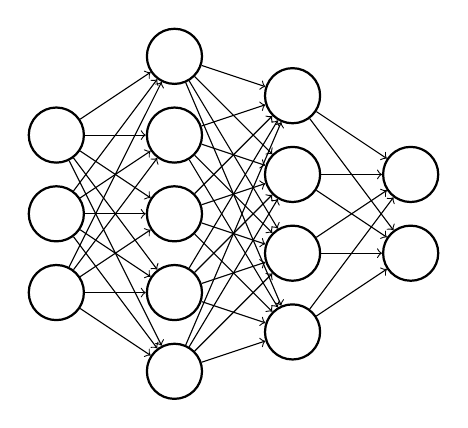
\begin{tikzpicture}[
    neuron/.style={circle, minimum size=.7cm, thick},
    tip/.style={->}
  ]
  % draw neurons
  \node[neuron, draw] at (-1.5,1) (11) {};
  \node[neuron, draw] at (-1.5,0) (12) {};
  \node[neuron, draw] at (-1.5,-1) (13) {};
  \foreach \n in {21,...,25}{
    \node[neuron, draw] at (0, \n - 23) (\n) {};}
  \foreach \n in {31,...,34}{
    \node[neuron, draw] at (1.5,\n-32.5) (\n) {};}
  \foreach \n in {41,...,42}{
    \node[neuron, draw] at (3.0,\n-41.5) (\n) {};}

  % draw connections
  \foreach \idx in {11,...,13}{
    \foreach \jdx in {21,...,25}{
      \path[draw,tip] (\idx) edge (\jdx) node {};}}
  \foreach \idx in {21,...,25}{
    \foreach \jdx in {31,...,34}{
      \path[draw,tip] (\idx) edge (\jdx) node {};}}
  \foreach \idx in {31,...,34}{
    \foreach \jdx in {41,...,42}{
      \path[draw,tip] (\idx) edge (\jdx) node {};}}
\end{tikzpicture}
}

    \column{.5\textwidth}\centering
    \textbf{Neural} Differential Equation:
    \begin{equation*}
      \begin{bmatrix}
        \dot S\\ \dot I\\ \dot R
      \end{bmatrix}
      = \mathrm{NeuralODE}\left(\begin{bmatrix}
        S \\ I \\ R
      \end{bmatrix}, \bm\theta
      \right)
    \end{equation*}
  \end{columns}
\end{frame}


\begin{frame}{Fractional SIR}
  \centering
  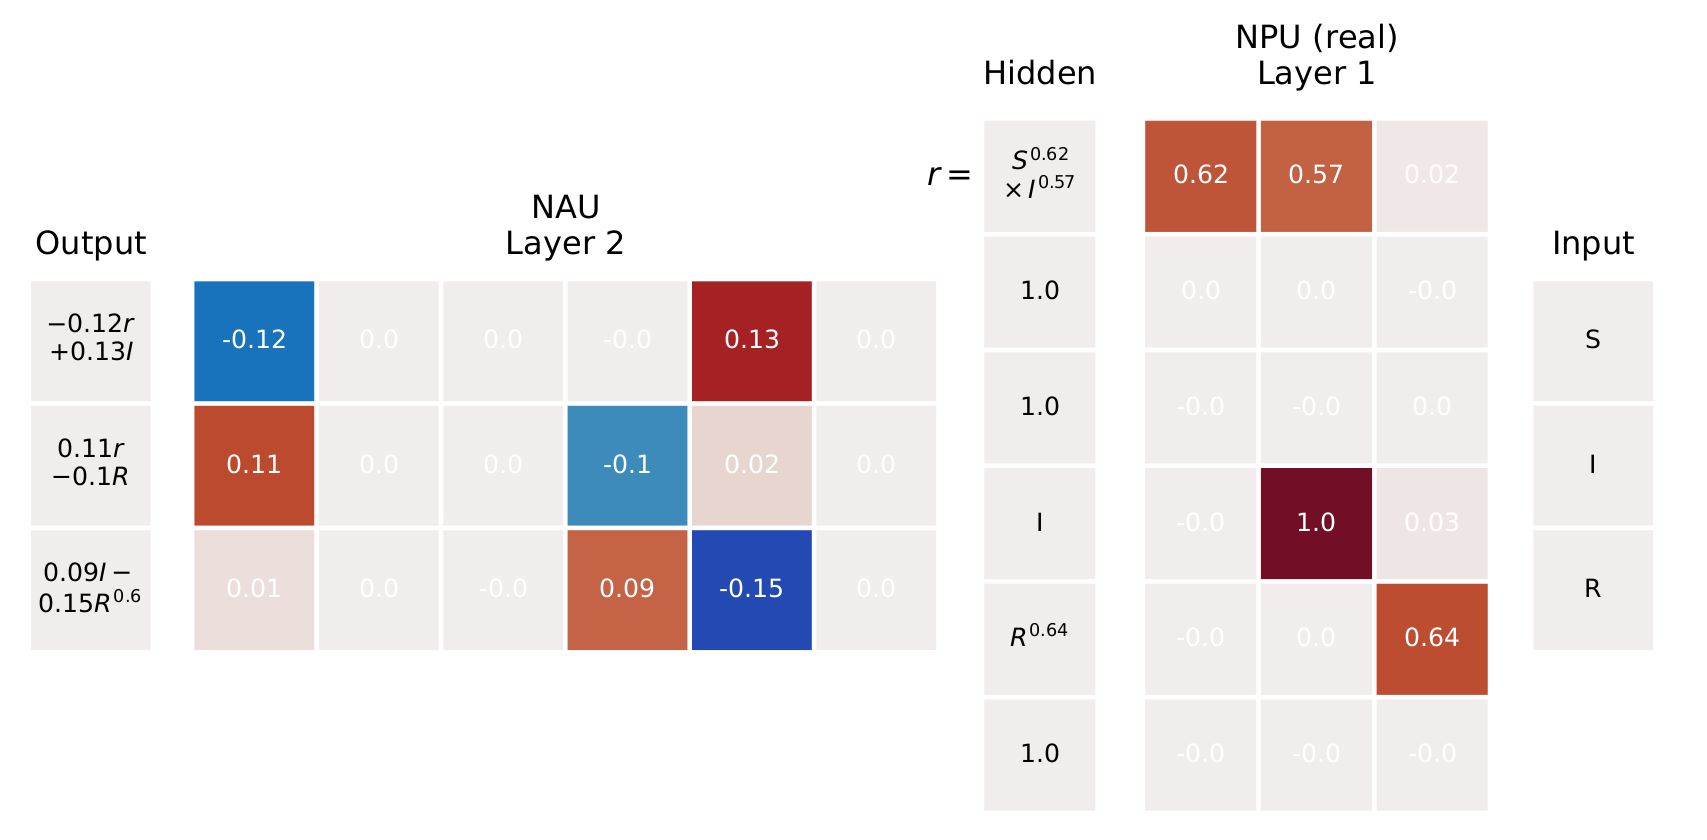
\includegraphics[width=.8\textwidth]{fsir-params.png}
  \begin{equation*}
    \begin{bmatrix}
      \dot S \\ \dot I \\ \dot R
    \end{bmatrix}
    =
    \begin{bmatrix}
      -\beta & 0 & \eta \\
      \beta & -\alpha & 0 \\
      0 & \alpha & -\eta
    \end{bmatrix}
    \begin{bmatrix}
      I^\gamma S^\kappa \\ I \\ R
    \end{bmatrix}
  \end{equation*}
\end{frame}

\begin{frame}{Future Work}
  \centering
  \begin{columns}
    \column{.5\textwidth}\centering
    \resizebox{!}{.6\textwidth}{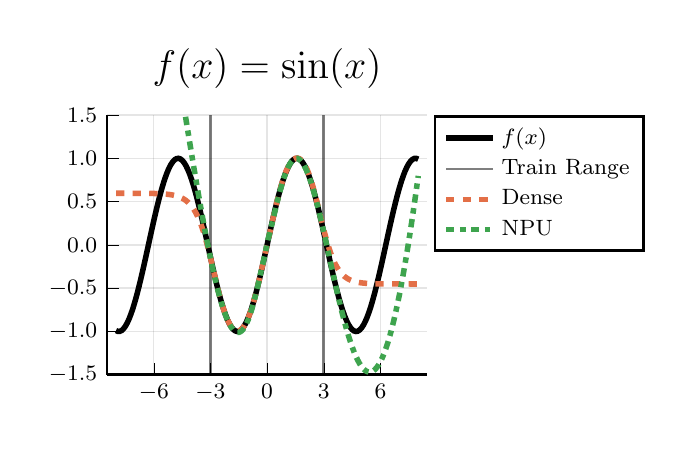
\begin{tikzpicture}[/tikz/background rectangle/.style={fill={rgb,1:red,1.0;green,1.0;blue,1.0}, draw opacity={1.0}}, show background rectangle]
\begin{axis}[point meta max={nan}, point meta min={nan}, legend cell align={left}, title={$f(x) = \sin(x)$}, title style={at={{(0.5,1)}}, anchor={south}, font={{\fontsize{14 pt}{18.2 pt}\selectfont}}, color={rgb,1:red,0.0;green,0.0;blue,0.0}, draw opacity={1.0}, rotate={0.0}}, legend style={color={rgb,1:red,0.0;green,0.0;blue,0.0}, draw opacity={1.0}, line width={1}, solid, fill={rgb,1:red,1.0;green,1.0;blue,1.0}, fill opacity={1.0}, text opacity={1.0}, font={{\fontsize{8 pt}{10.4 pt}\selectfont}}, at={(1.02, 1)}, anchor={north west}}, axis background/.style={fill={rgb,1:red,1.0;green,1.0;blue,1.0}, opacity={1.0}}, anchor={north west}, xshift={1.0mm}, yshift={-1.0mm}, width={56.5mm}, height={48.8mm}, scaled x ticks={false}, xlabel={}, x tick style={color={rgb,1:red,0.0;green,0.0;blue,0.0}, opacity={1.0}}, x tick label style={color={rgb,1:red,0.0;green,0.0;blue,0.0}, opacity={1.0}, rotate={0}}, xlabel style={at={(ticklabel cs:0.5)}, anchor=near ticklabel, font={{\fontsize{11 pt}{14.3 pt}\selectfont}}, color={rgb,1:red,0.0;green,0.0;blue,0.0}, draw opacity={1.0}, rotate={0.0}}, xmajorgrids={true}, xmin={-8.48}, xmax={8.48}, xtick={{-6.0,-3.0,0.0,3.0,6.0}}, xticklabels={{$-6$,$-3$,$0$,$3$,$6$}}, xtick align={inside}, xticklabel style={font={{\fontsize{8 pt}{10.4 pt}\selectfont}}, color={rgb,1:red,0.0;green,0.0;blue,0.0}, draw opacity={1.0}, rotate={0.0}}, x grid style={color={rgb,1:red,0.0;green,0.0;blue,0.0}, draw opacity={0.1}, line width={0.5}, solid}, axis x line*={left}, x axis line style={color={rgb,1:red,0.0;green,0.0;blue,0.0}, draw opacity={1.0}, line width={1}, solid}, scaled y ticks={false}, ylabel={}, y tick style={color={rgb,1:red,0.0;green,0.0;blue,0.0}, opacity={1.0}}, y tick label style={color={rgb,1:red,0.0;green,0.0;blue,0.0}, opacity={1.0}, rotate={0}}, ylabel style={at={(ticklabel cs:0.5)}, anchor=near ticklabel, font={{\fontsize{11 pt}{14.3 pt}\selectfont}}, color={rgb,1:red,0.0;green,0.0;blue,0.0}, draw opacity={1.0}, rotate={0.0}}, ymajorgrids={true}, ymin={-1.5}, ymax={1.5}, ytick={{-1.5,-1.0,-0.5,0.0,0.5,1.0,1.5}}, yticklabels={{$-1.5$,$-1.0$,$-0.5$,$0.0$,$0.5$,$1.0$,$1.5$}}, ytick align={inside}, yticklabel style={font={{\fontsize{8 pt}{10.4 pt}\selectfont}}, color={rgb,1:red,0.0;green,0.0;blue,0.0}, draw opacity={1.0}, rotate={0.0}}, y grid style={color={rgb,1:red,0.0;green,0.0;blue,0.0}, draw opacity={0.1}, line width={0.5}, solid}, axis y line*={left}, y axis line style={color={rgb,1:red,0.0;green,0.0;blue,0.0}, draw opacity={1.0}, line width={1}, solid}]
    \addplot[color={rgb,1:red,0.0;green,0.0;blue,0.0}, name path={b6a94104-d18d-42fc-8460-776c8180f288}, draw opacity={1.0}, line width={2}, solid]
        table[row sep={\\}]
        {
            \\
            -8.0  -0.98935825  \\
            -7.9  -0.99894136  \\
            -7.8  -0.9985434  \\
            -7.7  -0.9881682  \\
            -7.6  -0.96791965  \\
            -7.5  -0.93799996  \\
            -7.4  -0.89870816  \\
            -7.3  -0.85043675  \\
            -7.2  -0.79366773  \\
            -7.1  -0.728969  \\
            -7.0  -0.6569866  \\
            -6.9  -0.57843983  \\
            -6.8  -0.4941135  \\
            -6.7  -0.40484974  \\
            -6.6  -0.31154126  \\
            -6.5  -0.21511999  \\
            -6.4  -0.1165493  \\
            -6.3  -0.01681409  \\
            -6.2  0.08308959  \\
            -6.1  0.1821626  \\
            -6.0  0.2794155  \\
            -5.9  0.37387657  \\
            -5.8  0.46460202  \\
            -5.7  0.5506857  \\
            -5.6  0.6312667  \\
            -5.5  0.7055403  \\
            -5.4  0.77276444  \\
            -5.3  0.83226734  \\
            -5.2  0.88345474  \\
            -5.1  0.92581475  \\
            -5.0  0.9589243  \\
            -4.9  0.9824526  \\
            -4.8  0.9961646  \\
            -4.7  0.9999232  \\
            -4.6  0.99369097  \\
            -4.5  0.9775301  \\
            -4.4  0.9516021  \\
            -4.3  0.916166  \\
            -4.2  0.87157565  \\
            -4.1  0.81827706  \\
            -4.0  0.7568025  \\
            -3.9  0.68776625  \\
            -3.8  0.61185783  \\
            -3.7  0.5298362  \\
            -3.6  0.44252035  \\
            -3.5  0.35078323  \\
            -3.4  0.2555412  \\
            -3.3  0.15774564  \\
            -3.2  0.058374193  \\
            -3.1  -0.04158076  \\
            -3.0  -0.14112  \\
            -2.9  -0.23924923  \\
            -2.8  -0.3349882  \\
            -2.7  -0.42737985  \\
            -2.6  -0.51550144  \\
            -2.5  -0.5984721  \\
            -2.4  -0.67546314  \\
            -2.3  -0.74570525  \\
            -2.2  -0.80849636  \\
            -2.1  -0.8632094  \\
            -2.0  -0.9092974  \\
            -1.9  -0.9463001  \\
            -1.8  -0.9738476  \\
            -1.7  -0.9916648  \\
            -1.6  -0.9995736  \\
            -1.5  -0.997495  \\
            -1.4  -0.98544973  \\
            -1.3  -0.9635582  \\
            -1.2  -0.9320391  \\
            -1.1  -0.8912074  \\
            -1.0  -0.84147096  \\
            -0.9  -0.7833269  \\
            -0.8  -0.7173561  \\
            -0.7  -0.64421767  \\
            -0.6  -0.5646425  \\
            -0.5  -0.47942555  \\
            -0.4  -0.38941833  \\
            -0.3  -0.29552022  \\
            -0.2  -0.19866933  \\
            -0.1  -0.09983342  \\
            0.0  0.0  \\
            0.1  0.09983342  \\
            0.2  0.19866933  \\
            0.3  0.29552022  \\
            0.4  0.38941833  \\
            0.5  0.47942555  \\
            0.6  0.5646425  \\
            0.7  0.64421767  \\
            0.8  0.7173561  \\
            0.9  0.7833269  \\
            1.0  0.84147096  \\
            1.1  0.8912074  \\
            1.2  0.9320391  \\
            1.3  0.9635582  \\
            1.4  0.98544973  \\
            1.5  0.997495  \\
            1.6  0.9995736  \\
            1.7  0.9916648  \\
            1.8  0.9738476  \\
            1.9  0.9463001  \\
            2.0  0.9092974  \\
            2.1  0.8632094  \\
            2.2  0.80849636  \\
            2.3  0.74570525  \\
            2.4  0.67546314  \\
            2.5  0.5984721  \\
            2.6  0.51550144  \\
            2.7  0.42737985  \\
            2.8  0.3349882  \\
            2.9  0.23924923  \\
            3.0  0.14112  \\
            3.1  0.04158076  \\
            3.2  -0.058374193  \\
            3.3  -0.15774564  \\
            3.4  -0.2555412  \\
            3.5  -0.35078323  \\
            3.6  -0.44252035  \\
            3.7  -0.5298362  \\
            3.8  -0.61185783  \\
            3.9  -0.68776625  \\
            4.0  -0.7568025  \\
            4.1  -0.81827706  \\
            4.2  -0.87157565  \\
            4.3  -0.916166  \\
            4.4  -0.9516021  \\
            4.5  -0.9775301  \\
            4.6  -0.99369097  \\
            4.7  -0.9999232  \\
            4.8  -0.9961646  \\
            4.9  -0.9824526  \\
            5.0  -0.9589243  \\
            5.1  -0.92581475  \\
            5.2  -0.88345474  \\
            5.3  -0.83226734  \\
            5.4  -0.77276444  \\
            5.5  -0.7055403  \\
            5.6  -0.6312667  \\
            5.7  -0.5506857  \\
            5.8  -0.46460202  \\
            5.9  -0.37387657  \\
            6.0  -0.2794155  \\
            6.1  -0.1821626  \\
            6.2  -0.08308959  \\
            6.3  0.01681409  \\
            6.4  0.1165493  \\
            6.5  0.21511999  \\
            6.6  0.31154126  \\
            6.7  0.40484974  \\
            6.8  0.4941135  \\
            6.9  0.57843983  \\
            7.0  0.6569866  \\
            7.1  0.728969  \\
            7.2  0.79366773  \\
            7.3  0.85043675  \\
            7.4  0.89870816  \\
            7.5  0.93799996  \\
            7.6  0.96791965  \\
            7.7  0.9881682  \\
            7.8  0.9985434  \\
            7.9  0.99894136  \\
            8.0  0.98935825  \\
        }
        ;
    \addlegendentry {$f(x)$}
    \addplot[color={rgb,1:red,0.0;green,0.0;blue,0.0}, name path={1570e8e2-4e91-434e-89bb-3693e0cc7640}, draw opacity={0.5}, line width={1}, solid]
        table[row sep={\\}]
        {
            \\
            -3.0  -4.5  \\
            -3.0  4.5  \\
        }
        ;
    \addlegendentry {Train Range}
    \addplot[color={rgb,1:red,0.0;green,0.0;blue,0.0}, name path={1570e8e2-4e91-434e-89bb-3693e0cc7640}, draw opacity={0.5}, line width={1}, solid, forget plot]
        table[row sep={\\}]
        {
            \\
            3.0  -4.5  \\
            3.0  4.5  \\
        }
        ;
    \addplot[color={rgb,1:red,0.8889;green,0.4356;blue,0.2781}, name path={ce5cf13d-1d3c-4944-9e36-419049acf873}, draw opacity={1.0}, line width={2}, dashed]
        table[row sep={\\}]
        {
            \\
            -8.0  0.59659517  \\
            -7.9  0.596581  \\
            -7.8  0.596564  \\
            -7.7  0.59654456  \\
            -7.6  0.5965215  \\
            -7.5  0.5964941  \\
            -7.4  0.5964614  \\
            -7.3  0.5964223  \\
            -7.2  0.59637535  \\
            -7.1  0.5963181  \\
            -7.0  0.59624964  \\
            -6.9  0.5961662  \\
            -6.8  0.5960647  \\
            -6.7  0.595941  \\
            -6.6  0.5957904  \\
            -6.5  0.5956066  \\
            -6.4  0.5953819  \\
            -6.3  0.59510714  \\
            -6.2  0.5947711  \\
            -6.1  0.5943599  \\
            -6.0  0.5938562  \\
            -5.9  0.5932397  \\
            -5.8  0.5924847  \\
            -5.7  0.59156  \\
            -5.6  0.5904274  \\
            -5.5  0.58904105  \\
            -5.4  0.58734334  \\
            -5.3  0.5852656  \\
            -5.2  0.58272314  \\
            -5.1  0.5796146  \\
            -5.0  0.5758156  \\
            -4.9  0.57117665  \\
            -4.8  0.565518  \\
            -4.7  0.55862385  \\
            -4.6  0.55023724  \\
            -4.5  0.5400544  \\
            -4.4  0.52771825  \\
            -4.3  0.5128149  \\
            -4.2  0.4948699  \\
            -4.1  0.47334963  \\
            -4.0  0.44766593  \\
            -3.9  0.4171893  \\
            -3.8  0.38127244  \\
            -3.7  0.33928406  \\
            -3.6  0.29065967  \\
            -3.5  0.23496282  \\
            -3.4  0.17196107  \\
            -3.3  0.101702034  \\
            -3.2  0.024585396  \\
            -3.1  -0.058588  \\
            -3.0  -0.14660569  \\
            -2.9  -0.23788044  \\
            -2.8  -0.33053997  \\
            -2.7  -0.42255569  \\
            -2.6  -0.5119002  \\
            -2.5  -0.5966941  \\
            -2.4  -0.67532897  \\
            -2.3  -0.74653774  \\
            -2.2  -0.8094161  \\
            -2.1  -0.86339515  \\
            -2.0  -0.9081774  \\
            -1.9  -0.9436578  \\
            -1.8  -0.9698417  \\
            -1.7  -0.9867698  \\
            -1.6  -0.99446404  \\
            -1.5  -0.9928944  \\
            -1.4  -0.98197407  \\
            -1.3  -0.96157867  \\
            -1.2  -0.931595  \\
            -1.1  -0.89198667  \\
            -1.0  -0.842872  \\
            -0.9  -0.784594  \\
            -0.8  -0.717765  \\
            -0.7  -0.64326483  \\
            -0.6  -0.56218743  \\
            -0.5  -0.47573742  \\
            -0.4  -0.38510826  \\
            -0.3  -0.2913712  \\
            -0.2  -0.19541232  \\
            -0.1  -0.09793568  \\
            0.0  0.00047315657  \\
            0.1  0.099242836  \\
            0.2  0.19770825  \\
            0.3  0.29503143  \\
            0.4  0.39017475  \\
            0.5  0.48193574  \\
            0.6  0.5690304  \\
            0.7  0.6502043  \\
            0.8  0.72433996  \\
            0.9  0.7905383  \\
            1.0  0.8481573  \\
            1.1  0.89680564  \\
            1.2  0.9363034  \\
            1.3  0.9666183  \\
            1.4  0.987797  \\
            1.5  0.9999006  \\
            1.6  1.002955  \\
            1.7  0.99692154  \\
            1.8  0.98169136  \\
            1.9  0.95710564  \\
            2.0  0.9230025  \\
            2.1  0.8792887  \\
            2.2  0.8260288  \\
            2.3  0.76355016  \\
            2.4  0.69253194  \\
            2.5  0.6140735  \\
            2.6  0.5297091  \\
            2.7  0.4413551  \\
            2.8  0.3511932  \\
            2.9  0.26149416  \\
            3.0  0.1744262  \\
            3.1  0.09187305  \\
            3.2  0.015303493  \\
            3.3  -0.054292202  \\
            3.4  -0.11640191  \\
            3.5  -0.17093503  \\
            3.6  -0.21813786  \\
            3.7  -0.2584952  \\
            3.8  -0.29263854  \\
            3.9  -0.32126808  \\
            4.0  -0.34509623  \\
            4.1  -0.36480546  \\
            4.2  -0.38102412  \\
            4.3  -0.3943143  \\
            4.4  -0.4051671  \\
            4.5  -0.41400468  \\
            4.6  -0.4211849  \\
            4.7  -0.42700768  \\
            4.8  -0.43172228  \\
            4.9  -0.43553543  \\
            5.0  -0.43861663  \\
            5.1  -0.44110394  \\
            5.2  -0.4431113  \\
            5.3  -0.4447304  \\
            5.4  -0.4460354  \\
            5.5  -0.44708753  \\
            5.6  -0.44793522  \\
            5.7  -0.4486189  \\
            5.8  -0.44916975  \\
            5.9  -0.44961345  \\
            6.0  -0.44997156  \\
            6.1  -0.45025992  \\
            6.2  -0.45049262  \\
            6.3  -0.4506806  \\
            6.4  -0.4508325  \\
            6.5  -0.4509549  \\
            6.6  -0.4510541  \\
            6.7  -0.45113468  \\
            6.8  -0.4512  \\
            6.9  -0.45125294  \\
            7.0  -0.4512961  \\
            7.1  -0.4513315  \\
            7.2  -0.45136058  \\
            7.3  -0.45138443  \\
            7.4  -0.4514042  \\
            7.5  -0.45142066  \\
            7.6  -0.45143437  \\
            7.7  -0.45144618  \\
            7.8  -0.45145607  \\
            7.9  -0.45146453  \\
            8.0  -0.45147192  \\
        }
        ;
    \addlegendentry {Dense}
    \addplot[color={rgb,1:red,0.2422;green,0.6433;blue,0.3044}, name path={5fe89d8b-6086-457a-b8a5-44300de3873d}, draw opacity={1.0}, line width={2}, dashdotted]
        table[row sep={\\}]
        {
            \\
            -8.0  6.010978  \\
            -7.9  5.915226  \\
            -7.8  5.817529  \\
            -7.7  5.7178974  \\
            -7.6  5.6163483  \\
            -7.5  5.5128975  \\
            -7.4  5.4075594  \\
            -7.3  5.3003554  \\
            -7.2  5.1913104  \\
            -7.1  5.080448  \\
            -7.0  4.967796  \\
            -6.9  4.8533874  \\
            -6.8  4.7372546  \\
            -6.7  4.6194324  \\
            -6.6  4.499963  \\
            -6.5  4.3788896  \\
            -6.4  4.256258  \\
            -6.3  4.132122  \\
            -6.2  4.0065336  \\
            -6.1  3.8795538  \\
            -6.0  3.7512445  \\
            -5.9  3.621674  \\
            -5.8  3.4909163  \\
            -5.7  3.3590474  \\
            -5.6  3.2261512  \\
            -5.5  3.0923173  \\
            -5.4  2.9576383  \\
            -5.3  2.8222156  \\
            -5.2  2.6861548  \\
            -5.1  2.549571  \\
            -5.0  2.4125848  \\
            -4.9  2.2753227  \\
            -4.8  2.1379197  \\
            -4.7  2.0005183  \\
            -4.6  1.8632718  \\
            -4.5  1.7263393  \\
            -4.4  1.5898892  \\
            -4.3  1.4541004  \\
            -4.2  1.3191592  \\
            -4.1  1.1852655  \\
            -4.0  1.0526266  \\
            -3.9  0.9214608  \\
            -3.8  0.7920008  \\
            -3.7  0.66448474  \\
            -3.6  0.5391677  \\
            -3.5  0.41631633  \\
            -3.4  0.29620516  \\
            -3.3  0.17912793  \\
            -3.2  0.065384865  \\
            -3.1  -0.044706583  \\
            -3.0  -0.15081918  \\
            -2.9  -0.25261182  \\
            -2.8  -0.3497312  \\
            -2.7  -0.44181216  \\
            -2.6  -0.528478  \\
            -2.5  -0.60934204  \\
            -2.4  -0.68401  \\
            -2.3  -0.75207883  \\
            -2.2  -0.81313974  \\
            -2.1  -0.8667824  \\
            -2.0  -0.9125969  \\
            -1.9  -0.95017934  \\
            -1.8  -0.97913384  \\
            -1.7  -0.999084  \\
            -1.6  -1.0096785  \\
            -1.5  -1.0105984  \\
            -1.4  -1.0015744  \\
            -1.3  -0.9823978  \\
            -1.2  -0.9529427  \\
            -1.1  -0.9131857  \\
            -1.0  -0.8632354  \\
            -0.9  -0.80336857  \\
            -0.8  -0.7340719  \\
            -0.7  -0.656093  \\
            -0.6  -0.5705137  \\
            -0.5  -0.47882432  \\
            -0.4  -0.38303426  \\
            -0.3  -0.28579828  \\
            -0.2  -0.190582  \\
            -0.1  -0.101870045  \\
            0.0  0.024224237  \\
            0.1  0.10692157  \\
            0.2  0.19462949  \\
            0.3  0.28515452  \\
            0.4  0.37638572  \\
            0.5  0.46634504  \\
            0.6  0.5532244  \\
            0.7  0.63540864  \\
            0.8  0.71148944  \\
            0.9  0.780269  \\
            1.0  0.84075946  \\
            1.1  0.8921756  \\
            1.2  0.9339248  \\
            1.3  0.96559507  \\
            1.4  0.9869408  \\
            1.5  0.9978676  \\
            1.6  0.9984182  \\
            1.7  0.9887565  \\
            1.8  0.96915376  \\
            1.9  0.9399736  \\
            2.0  0.90165997  \\
            2.1  0.85472274  \\
            2.2  0.7997292  \\
            2.3  0.73729104  \\
            2.4  0.66805434  \\
            2.5  0.59269273  \\
            2.6  0.5118971  \\
            2.7  0.42637062  \\
            2.8  0.3368209  \\
            2.9  0.24395485  \\
            3.0  0.14847273  \\
            3.1  0.051066548  \\
            3.2  -0.047588944  \\
            3.3  -0.14683318  \\
            3.4  -0.24602652  \\
            3.5  -0.34455353  \\
            3.6  -0.4418199  \\
            3.7  -0.5372603  \\
            3.8  -0.6303344  \\
            3.9  -0.72053057  \\
            4.0  -0.80736697  \\
            4.1  -0.8903892  \\
            4.2  -0.9691738  \\
            4.3  -1.0433261  \\
            4.4  -1.1124802  \\
            4.5  -1.1763012  \\
            4.6  -1.2344819  \\
            4.7  -1.2867434  \\
            4.8  -1.3328351  \\
            4.9  -1.3725322  \\
            5.0  -1.4056377  \\
            5.1  -1.4319816  \\
            5.2  -1.4514155  \\
            5.3  -1.4638176  \\
            5.4  -1.4690877  \\
            5.5  -1.4671495  \\
            5.6  -1.4579475  \\
            5.7  -1.4414468  \\
            5.8  -1.4176304  \\
            5.9  -1.3865038  \\
            6.0  -1.3480868  \\
            6.1  -1.3024173  \\
            6.2  -1.2495501  \\
            6.3  -1.1895536  \\
            6.4  -1.1225122  \\
            6.5  -1.0485221  \\
            6.6  -0.9676949  \\
            6.7  -0.8801496  \\
            6.8  -0.7860197  \\
            6.9  -0.68544996  \\
            7.0  -0.5785893  \\
            7.1  -0.46560213  \\
            7.2  -0.34665856  \\
            7.3  -0.22193336  \\
            7.4  -0.0916107  \\
            7.5  0.044117242  \\
            7.6  0.18505529  \\
            7.7  0.33100212  \\
            7.8  0.48175544  \\
            7.9  0.6371002  \\
            8.0  0.79682493  \\
        }
        ;
    \addlegendentry {NPU}
\end{axis}
\end{tikzpicture}
}

    \column{.5\textwidth}\centering
    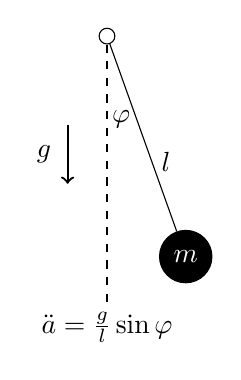
\begin{tikzpicture}
      \node[draw,circle,inner sep=0, minimum size=0.2cm] (top) at (0,0) {};
      \node[draw,circle,fill=black] (m) at (1,-2.8) {\color{white}{$m$}};
      \node (l) at (0.75,-1.6) {$l$};
      \node (p) at (0.18,-1.05) {$\varphi$};
      \node (mid) at (0,-3.5) {};
      \node (g1) at (-0.5,-1) {};
      \node (g2) at (-0.5,-2) {};
      \node (g) at (-0.8,-1.5) {$g$};
      \node (eq) at (0,-3.7) {$\ddot a = \frac{g}{l}\sin\varphi$};

      \path [draw,dashed] (top)  --  (mid);
      \path [draw] (top)  -- (m);
      \path [draw,->,thick] (g1) -- (g2);
    \end{tikzpicture}

  \end{columns}
  \vspace{0.3cm}
  \begin{columns}
    \column{.5\textwidth}\centering
    Trigonometric functions
    \column{.5\textwidth}\centering
    Some serious equation discovery
  \end{columns}

  \vfill
  \pause
  {\bf Do you have an application?}
\end{frame}



\begin{frame}
  \centering
  {\huge\bf Neural Arithmetic} \\
  \vspace{.5cm}
  \textbf{Extrapolating} Beyond The Training Range \\
  \& Building \textbf{Transparent} Models
  \vfill

  \begin{columns}
    \column{.33\textwidth}{
      \circleimage{1.5cm}{niklas.png}
      \begin{center} Niklas Heim \end{center}
    }
     \column{.33\textwidth}{
       \circleimage{1.5cm}{tomas.jpg}
       \begin{center} Tom\'a\v s Pevn\'y \end{center}
    }
    \column{.33\textwidth}{
      \circleimage{1.5cm}{vasek.png}
      \begin{center} V\'aclav \v Sm\'idl \end{center}
    }
  \end{columns}
  \vfill

  \vfill
  {\small \url{https://github.com/nmheim/NeuralArithmetic.jl}}\\
  {\small \url{heimnikl@fel.cvut.cz}}
\end{frame}

\end{document}
